\documentclass[11pt,proposal,double]{pitthesis}
%\documentclass[11pt,proposal,double,draft]{pitthesis}


%packages
%\usepackage{subfiles}
%\usepackage{graphicx}
\usepackage[final]{graphicx}
\usepackage{xcolor}
\usepackage{subcaption}
%\usepackage{subfigure}
\usepackage{hyperref}
\usepackage{setspace} %single spacing
\usepackage[]{pdfpages} %single spacing
\hypersetup{
    colorlinks=true, % make the links colored
    linkcolor=blue, % color TOC links in blue
    urlcolor=red, % color URLs in red
    linktoc=all % 'all' will create links for everything in the TOC
}

\newif\ifAMS
  \IfFileExists{amsfonts.sty}
    {\AMStrue\usepackage{amsmath,amsthm,amsfonts}}
    {\usepackage{latexsym}}


% Declares the document's title.
\title{\bf Design of Small, Inexpensive, Environmentally Adaptable Robotic Platforms for Monitoring Applications}
\proposal{Written Preliminary Exam } % print on title page by 'proposal' option
\author{Dario J. Canelon}			% Declares the author's name.

% Declares formerly earned degrees
\degrees{B.S. in M.E., University of Minnesota, Twin Cities, 2009}

% Declares degree to earn
\degree{Doctor\\of\\Philosophy}
%\degree{Master of Science\\in\\Electrical Engineering} % for M.S.

\school{Department of Mechanical Engineering}		% for School of Engineering thesis
\university{University of Minnesota}	% the University

\date{}
\year{}		% year in title page

\includeonly{
  parts/cover_page,
  %parts/ackn,
  project_summary,
  project_description,
  parts/appendix,
  parts/biosketch,
  }


%%---------------------------------------------------------------------------
\begin{document}
%%---------------------------------------------------------------------------

\maketitle		% Produces the title.

\begin{committeesignature}[4]

%% For Ph.D. Thesis
\advisor{Nikolaos Papanikolopoulos, Professor (Mechanical Engineering). Reader.}
\committeemember{Rajesh Rajamani, Professor (Mechanical Engineering). Reader.}
\committeemember{Timothy Kowalewski, Associate Professor (Mechanical Engineering). Reader.}
\committeemember{Junaed Sattar, Assistant Professor (Computer Science and Engineering)}
\end{committeesignature}	% end the committee signature page.


\include{parts/ackn}

\advisorname{Nikolaos Papanikolopoulos, Professor}   % for PhD thesis abstract page
%\abstract		% generate the heading of abstract page

\tableofcontents
%\listoffigures
%\listoftables

% Summary page 
\chapter{Project Summary}
%Project Summary.

%The Project Summary is a one page, single-spaced summary of the proposed
%activity. The Project Summary should be a self-contained
%description of the proposed research. It should include a statement of
%objectives and methods to be employed. It must address the scientific and/or
%technical merit of the project, for example, the influence that the results
%might have on the direction, progress and thinking in relevant scientific or
%engineering fields.

%It must also address the appropriateness of the proposed methods, and the
%logic and feasibility of the research approach.  The Project Summary should be
%informative to persons working in the same or related fields and, insofar as
%possible, understandable to a scientifically or technically literate lay
%reader.
%%%%%%%%%%%%%%%%%%%%%%%%%%%%%%%%%%%%%%%%%%%%%%%%%%%%%%%%%%%%%%%%%%%%%%%%%%%%%%%%

\begin{singlespace}
  

%The automation of tasks that are dangerous, inconvenient, or otherwise undesirable for humans are one of the main benefits of intelligent and programmable robots. 
Environmental monitoring is a field that could benefit greatly from efforts in automation as the dynamic and spatially transient properties of natural phenomena can be difficult or costly to carry out via traditional human intensive methods. 

We propose research into the design of small environmentally adaptable robotic platforms to expand available methods for environmental monitoring with the objective of increasing the quality and quantity of data collection through greater automation. 

Towards that general goal we identify certain traits to focus on. Multi-domain operation to expand the scope of measurements. Field deployability as platforms are, ideally, designed to function robustly in real-world scenarios. In order to promote use and adoption, these platforms should complement existing methods used by scientists as well as be easy to use, configure, and deploy in the field. 

We propose developing a land-water robot for assisting water quality measurements and oil slick detection to depths of up to 10 meters and capable of expansion via "backpack" modules, such as a water sampling backpack or a volumetric particle counting sensor. 

We also propose the research and development of an amphibious method of locomotion for small robotic platforms. The screwdrive would allow a platform to locomote and transition seamlessly between land and water domains, increasing the robot's adaptibility. This method of locomotion is relatively unexplored, particularly for robotics, yet it is uniquely positioned to fulfill the amphibious space while being simple in design. 

Prior research on large military tank-size screwdrive propulsion systems indicates that optimal screw parameters, such as blade height and pitch, differ for land and water regimes, therefore, characterization at this scale is necessary. Furthermore, we propose the development of a variable-pitch screw to be used in this system both for characterization purposes and for field deployment. One way to achieve this would be the use of origami or kirigami to induce buckling along predefined creases where actuation morphs the geometry of the screw a manner akin to the way an accordion expands and contracts, changing its properties. In order to match the variable screws to their terrain, a terrain classification system is also proposed.  

Finally, noting the benefits of land-water adaptability to the available mission set, we propose development of a land-water-air platform that incorporates principles from the land-water platform, the amphibious powertrain, and adds flight capabilities. This new platform, to the author's knowledge, would be the first of its kind. The addition of flight would allow quicker and easier deployment and retrieval while allowing sensing methodologies not previously available.

%Finally, we propose the development of a land-water-air platform that incorporates principles from the Aquapod, the screwdrive, and adds flight. This new platform, to the author's knowledge, would be the first of its kind. This platform would allow quicker deployment using flight to overcome obstacles while still being able to perform measurement tasks. 

\end{singlespace} % one-page
%\includepdf[pages=-]{project_summary_standalone.pdf}

% Project 
\chapter{Project Description}
%Project Description. The Project Description is a 30 page (maximum), double-spaced proposal that describes the thesis project. It should include motivation and objectives, background, proposed research, preliminary results, and conclusion. The organization of the document is up to the student, in consultation with the adviser(s). Figures and tables are included in the 30 page limit.

Mobile robotic platforms are increasingly being used as a substitute to human correspondence for search and rescue, environmental monitoring, and other applications where automation is desirable due to hazardous conditions, convenience, repetitive nature of the task, or improved efficacy of resource usage. 

%TODO: how many lakes exactly
%TODO: change so it reads 'environmentally adaptable robots"
Water quality monitoring is important to Minnesota and the health of its more than 10,000 lakes. There is an opportunity to assist researchers in environmental monitoring efforts by developing inexpensive robots that are capable of augmenting data collection efforts and providing tools that reduce the amount of time and costs associated with it. this data collection. 

The ability of a mobile robot to carry out its mission will depend on a number of, often, competing factors, not least of which are the ability to navigate an environment, run time, weight, size, cost, as well as sensor and payload capabilities. Careful balancing of these design factors can lead to solutions that are more than the sum of the parts, enabling unique capabilities not previously available.

\section{Background and Motivation}
	\label{sec:background_and_motivation}

	% Background and Motivation
	% The background & motivation section should include a critical review of the relevant literature. It should indicate the current state of understanding of the proposed research topic. The review should emphasize how the prior work relates to the proposed study. It should address the significance and limitations of the cited work. If any figures are taken from another publication or a website, they must be referenced explicitly in the caption.

	Robotic platforms have the potential to aid researchers in a number of ways.  From assisting in data collection, to monitoring toxicity levels in disaster scenarios, to inspection of access-limited locations or objects, the possibilities are endless. Utilizing robots to monitor an environment through strategic placement, leverage the mobility of these nodes to obtain a more comprehensive understanding of the problem at hand. 

	\subsection{Environmental Monitoring via Robotic Platforms}%----------------------------------------------------------------

		In events from the Horizon Oil Spill \cite{dssoa} to the Fukushima Nuclear Disaster \cite{Hasegawa2012}, robotic platforms have permitted monitoring of environmental conditions and the completion of vital tasks while reducing the need to place human resources in danger. In the case of environmental monitoring, the long-term goal is to deploy a number of robots to carry out sensory tasks in an automated fashion, sometimes spanning days or weeks, with occasional human interaction for maintenance or supervision.

	%	Water quality of aquatic environments is of critical importance for a variety of economic, environmental, and public health reasons. 
		The economies of many regions around the globe are closely linked to the ability to use water resources for fishing, farming, crop irrigation, and tourism. There are several sources of contamination that can cause millions of dollars in damages including harmful algal blooms (HABs) and oil spills \cite{EPA2015a}. Hitz et al. \cite{Hitz2012} designed an autonomous surface vehicle (ASV), named Lizhbeth,  to monitor the temporal-spatial properties of lacustrine environments. The 120 kg robot has been tested been succesfully tested in Lake Zurich. 
		%Similarly, Greenfield et al. have developed an ASV to perform laboratory-type measurements of algae in the field \cite{Greenfield2008}. This special machine, called the Environmental Sampling Processor (ESP), concentrates and filters physical samples to then utilize DNA probing in order to perform tasks such as species identification, particulate concentration, among others. %CUT: Dunbabin et al. \cite{Dunbabin2009} have used a solar powered catamaran to autonomously navigate complex inland body of water and relevant data. It uses GPS for autonomous navigation and is capable of integration with an existing buoy sensor network which provide a number of additional features, among them bidirectional communications with its operators.  

		In other cases, researchers have turned to aerial platforms to deploy specific sensors to strategic locations and intelligently gather data of the underlying physicochemical properties of the environment. Ore et al. \cite{Ore2015} employed a slung-load waterproof micropump from a commercial AscTec Firefly drone. The pump is at the end of flexible tubing that is used to collect 20 mL samples as the drone hovers up to 1 meter over the water. 
		
		%Utilizing small mobile platforms that integrate proportionately smaller sensors allows the active collection of information in a way that is not available by laboratory testing of samples or stationary sensors. Furthermore, active sensors that process data \emph{in situ} enable live feedback data to collect data in a more efficient and accurate manner such as done by Neumann et al. \cite{Neumann2012}, where an "artificial potential field" is created to guide the next measurements of their microdrone. 
		
%cancut
	
	\subsection{Locomotion}%-----------------------------------------------------------------
	%TODO: go through this section towards the end
	\label{sec:locomotion} 

		Mobile robotic platforms, by definition, have to effectively move about their environment. Mobility allows exploration of new and unknown environments, sensor placement, data collection, among many other applications. Therefore, it follows that mobility is a major consideration when designing a robot and a major area of research. 

		Wheeled-robots, such as the Scout \cite{Rybski2000}, are well-known and studied \cite{Soetanto2003}. Some research in this area has focused on adding additional actuators to overcome difficult terrain or obstacles. Stoeter et al. \cite{Stoeter2006} enable jumping through a spring-loaded tail that is pulled closed by a winch and released to effectuate a jump. %Controlled wheel motion is used until an obstacle is encountered, at which point the jumping mechanism is deployed. 

		The Mini-Wheg \cite{Morrey2003} features a tri-spoke rimless wheel design that permits speeds of up to 10 body lengths per second while their open design allows surpassing obstacles. The incorporation of a four-bar-linkage jumping mechanism allows the robot to jump an average stair step. Similar in concept, yet much bigger, the Loper robot \cite{Herbert2008} has tri-lobe wheels and a flexible chassis to overcome uneven terrain or obstacles. The Loper has a top speed of 4.3 body lengths per second and can climb stairs at a rate of 6 steps per second \cite{Herbert2009}.  

		%CUT: The EPFL family of robots \cite{MirkoKovac2010} weigh between 7 and 14.3 grams and are capable of jumps 27 times their height all using onboard actuators and energy storage. The EPFL jumpglider was created by adding gliding and limited steering while keeping weight under 16.5 grams.

		%CUT: Birkmeyer et al. \cite{Birkmeyer2013} created a set of robotic platforms whose purpose was to explore the dynamics of vertical or near-vertical surface climbing. The DASH and CLASH platforms are cleverly designed with one miniature DC motor driving two alternating sets of three legs. Tripod gait is employed to climb loose cloth, vertical acrylic, and to study the dynamics of this task. 

		The RHEX platform \cite{Saranli2001a} is a hexapod robot that employs a clock-driven tripod gait. The six actuators are utilized to devise control strategies, capture model dynamics, and identify relevant parameters for robust traversal of rugged terrain and top speeds of up to one body-length per second. %Unlike the hexapedal DASH and CLASH \cite{Birkmeyer2013}, the RHEX utilizes one actuator per leg. 

		While land-based mobile robots were first and by far the most numerous, for technological and practical reasons, there are many robots designed specifically for water \cite{Villanueva2013} \cite{Yu2018} or air \cite{Neumann2012} \cite{Morton2013}.  
		
		Robots have been designed to operate in more than one domain, these are known as multi-domain robots. The snake robot AmphiBot I \cite{Crespi2005a}, the AQUA \cite{Dudek2007}, and the Whegs\texttrademark IV \cite{Boxerbaum2005} can traverse both land and water environments. The aquatic spherical robot Groundbot \cite{Kaznov2010} uses terrain-body interactions as its primary form of locomotion through rolling while its sealed hull allows it to travel atop the water.

	
	\subsection{The Adelopod and Aquapod RC}
  %-----------------------------------------------------------------
	\label{sec:adelopod_aquapodrc}
	%TODO: go through this section towards the end


		Tumbling locomotion, first presented formally in the Adelopod \cite{Hemes2009}, is a method of locomotion that increases the terrainability of a given platform. It does this by effectuating tumbles that leverage body of the robot to overcome obstacles that are larger, relative to its body, than what would be possible through a comparably sized wheeled solution \cite{Hemes2011}, thereby increasing traversability. The unsteady transition incurred during each tumble makes the outcome difficult to estimate in anything but a perfectly modeled environment, i.e. in any real-world scenario. 
		
		%Any unmodeled feature in the terrain greatly affects the outcome of the tumble. Moreover, even within \emph{in silico} conditions, input-output mapping necessitates non-trivial computational resources to find the correct sequence of coupled arm rotations to get within a bounded range of a desired target destination \cite{Hemes2008}. 

		%To overcome these challenges inherent to tumbling locomotion, tank-like treads were added to the Adelopod. Two small DC motors were added to the platform resulting in a small increase in size, however, independent actuation now allowed holonomic motion. The dual system permits navigation and path planning via the treads and then engagement of tumbling to overcome obstacles or irregular terrain. 

		The Aquapod RC \cite{Carlson2011} was envisioned with transitional land-water environments in mind. These areas are often difficult to traverse due to the presence of water and its effect on unprotected electronics and also from a locomotion perspective. Tumbling was chosen as primary method of locomotion due to its ability to cope with the unstructured and obstacle-laden nature of the terrain. This implied keeping the external shape and arms of the Adelopod. 
		
		To maintain the interior components safe from water ingression, the main seal was comprised of two custom-machined polycarbonate shells which sandwiched a matching Buna-N gasket. The power switch was located in a rectangular port on one corner of the robot behind a flexible rubber cover that allowed toggling the switch on and off without having to open the shell. The motor-arm interface was protected from water ingress by shaft seals pressed against recesses in the shell.  

		%Being that all the components, except for the arms, were located inside the shell, the remaining point of possible water ingress was the connection between the motors and the arms. Unlike the other static seals, the motor-arm interface required a shaft seal that was compressed against a cavity on either side of the robot.

		The ability to control the robot's density was another key feature for the Aquapod, this was accomplished via a buoyancy control unit (BCU). Unlike the ballast system used in submarines, the BCU ingests and expels water into a small bladder using a small peristaltic pump. The density is then altered since the shell volume remains constant. %This system assumes the robot starts positively buoyant and that the bladder capacity is large enough to make the robot negatively buoyant. 

		The Aquapod RC is commanded using a remote control that sends FM signals to a small receiver within the robot. This receiver, in turn, is connected to two electronic speed controllers (ESC) that each send a modulated voltage input to each of the DC motors that drive the arms and to the peristaltic pump. The radio frequency remote control is effective within line of sight but cannot effectively penetrate water. 

		With the proper modifications, such as propioceptive capabilities, an onboard computer, as well as external sensors, the Aquapod RC could become a capable robotic platform capable of adding autonomy to tasks that are currently difficult or time consuming for humans. 


	%TODO: add SAFL material ?




\section{Objectives}
%Objectives
%The objectives section should provide a context for the proposed work as well as specific objectives and expected significance of the Ph.D. dissertation. It should contain a brief overview of the proposed work in relation to the present state of knowledge in the field and to work in progress by others.

The overall objective of this work is to create robotic platforms that assist in environmental monitoring tasks. This has been organized into three distinct sections to better reflect the physical instatiations developed towards the achievement of the overall goal. 

\subsection{Aquapod}

% MRI RAPID https://www.nsf.gov/awardsearch/showAward?AWD_ID=1061489 

Shortly after the completion of the Aquapod RC, the Deepwater Oil Spill disaster occurred and a Major Research Instrumentation grant was awarded by the National Science Foundation to develop groups of Aquapods to help in the assessment of oil spill impact on marshlands surrounding the Gulf of Mexico. This provided a great opportunity to take the Aquapod concept and apply it to a real-world scenario. After consultation with a team of research biologists, it was determined that detection of subsurface oil-slick detection would be a key capability. The proposed solution would employ the Aquapods to collect electric conductivity profiles in the water column, the researcher would then look at these values, and program the sampling depths into the Aquapod. The Aquapod would then dive and take samples, all while collecting depth, temperature, and conductivity data.  

The overall goal was to create easy-to-use and robust platform that researchers could use to take sensor measurements and fluidic samples in a column of water. The automation of this process would allow researchers to more easily carry out a task that would otherwise be prohibited due to human cost or inconvenience. With this in mind, the objectives were to: 

\begin{itemize}
	\item \emph{Improve Robustness:} It was determined that 10 meters would be more than sufficient to detect subsurface oil slicks. Quantifying the depth rating of the Aquapod RC and making adjustments if necessary. 
	\item \emph{Add Sensing:} Conductivity, pressure, and temperature sensing, as well as subsurface fluid sampling were desirable. 
	\item \emph{Add Programmability:} to carry out subsurface sampling (where RC signals don't penetrate), but also to implement a state machine that would direct actions such as sampling and control buoyancy.
	\item \emph{Make an Easy to Use Interface:} An easy to use interface that would be simple enough to work out on the field but also be able to carry out commanded tasks. 
	\item \emph{Enhance Electronics:} Addition of a sacrificial fuel gauge board that monitors current usage and intervenes in case of a short circuit to protect other parts of the robot. Fuel gauge also allows charging of multi-cell Lithium Polymer batteries. 
\end{itemize}


\subsection{Screwdrive}

While tumbling is a desirable method of locomotion due to its mobility-to-size attributes, it also presents challenges for the amphibious Aquapod. Firstly, the shortcomings of tumbling are more pronounced underwater where the buoyant weight of the robot amplifies the tumbling unpredictability. Secondly, tumbling does not provide actuation while in suspension due to its reliance on interaction with a hard surface. For the Aquapod to travel to a location within a lake, it must try to tumble along the lakebed then surface. Obviously this presents numerous problems since GPS is not available underwater, there are multiple obstacles underwater, and underwater localization is an open problem, especially for small and inexpensive platforms.

Therefore, the need arose for an alternative mode of locomotion that would replace or complement tumbling. This mode of locomotion would have to:

\begin{itemize}
	\item \emph{Amphibious Function:} Capability to operate optimally both on land and in water. 
	\item \emph{Aquapod Compatibility:} Create a prototype in such a way as to complement and not compromise key attritubes of the Aquapod such as weight, size, and cost. 
	\item \emph{Characterization:} Study and develop prototypes to quantify the function of screwdrive systems for relatively light and small loads. 
	%\item \emph{Variable Geometry Screws:} Study and develop methods by which to vary the pitch of the screw blade both for characterization and on the fly parameter manipulation.
	\item \emph{Origami Construction:} Research Origami and Kirigami techniques to induce controlled traverse buckling of a screw body or blade to modify the screw's parameters, such as pitch, diameter, blade height, among others. 
\end{itemize}
	

\subsection{Omnibot}

Robotic platforms that can operate on multiple domains can offer numerous advantages compared to their single-domain counterparts. Unlike land or water platforms, aerial platforms require a large power-to-weight ratio to fly, this is limiting as it means that craft have to be very light, limiting materials that can be used as well as payload and sensor capabilities, or powerful, which implies large actuators and higher capacity for energy storage, often both. That being said, flight gives an unparalleled ability to navigate an environment, allows faster point to point navigation, and simpler deployment. Flight also allows visual inspection of an area at a scale and vantage not possible otherwise.

To the author's knowledge, a craft that is capable of navigation in land, in water, and air does not yet exist and there are design challenges to be solved in order to create one. The most significant challenge would be to balance the requirements of all three domains. Flight requires weight optimization of all components and the structure of the craft itself.  Water operation requires an enclosed and hermetic hull capable of handling the appropriate pressures. Actuator constraints are also significant as the torque and speed requirements for air, water, and land are very different. However, an environmentally-adaptable platform capable of all three domains would offer great flexibility during data collection. The range of measurements be expanded greatly, with reduced deployment times, and faster navigation to the desired measurement locations. Morever, a robot capable of operating in all three environments would be recoverable from all environments as well, further increasing its survivability and robustness. Specifically we propose: 
%A craft like this could land in the water to conserve energy while waiting to take the next set of measurements and then autonomously rendevous with a researcher. 

\begin{itemize}
	\item \emph{Design:} Study the design factors involved in a craft capable of operating in the land, water, and air requirements and their often-contradicting design requirements. 
	\item \emph{Transitions:} Study design considerations for environment to environment transitions (water-air, water-land, land-air). 
	\item \emph{Prototype}: The construction of a prototype that is able to carry a payload, achieve flight, navigation in water and land, as well as transition between the different terrain modalities. 
\end{itemize}

\section{Proposed Research} 
%This section should outline the plan of work, including the activities to be undertaken, and a description of experimental and/or computational methods and procedures. It should address what will be done, how it will achieve the proposed objectives, and should contain justification for the approach proposed. The proposed research section should complete the arguments developed earlier and present initial ideas on how to solve the problems posed. Strong proposals avoid repetition and digression. This section (or sections) should relate the proposed activities to the project objectives and provide expected outcomes, including how the proposed research, if successful, will contribute to a greater understanding of the topical area. An assessment of risk should be provided with the proposed research as well as a contingency plan in case a particular research avenue proves inexpedient in some manner. It should present a reasoned path from where the student begins to where they want to be at the end of the research.

In the following sections three different but related areas of research will be presented that focus on robots for environmental monitoring. In the first section an inexpensive land-water robot is proposed to aid with water quality monitoring, the Aquapod. Then, in the next section, the Screwdrive is presented as an amphibious method of locomotion. Then a first-of-its-kind platform capable of land, water, and air function is proposed, the Omnibot. By leveraging concepts from the Aquapod and the Screwdrive, we propose the study of the design of this platform. 

\subsection{The Aquapod Robotic Platform}
%\subsection{The Aquapod V1}
\label{sec:aquapod_results}

% Combined image  
\begin{figure}[!hb]
	\begin{subfigure}[t]{0.5\textwidth}
		\centering
		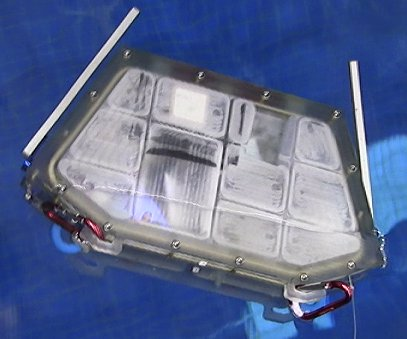
\includegraphics[width=1\columnwidth]{images/aquapod_v1_pool.jpg}
		\vspace{-10pt}
		\caption{Aquapod diving well test}
		%\vspace{-20pt}
		\label{fig:aquapod_pool}
	\end{subfigure}
	\begin{subfigure}[t]{0.5\textwidth}
		\centering
		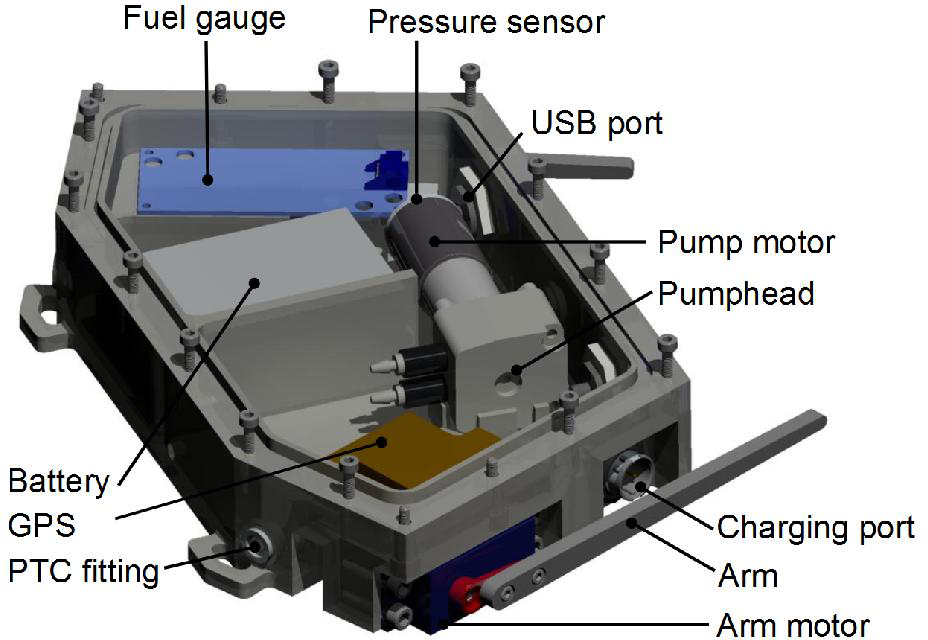
\includegraphics[width=1\columnwidth]{images/aquapod_v1_annotated.png}
		\vspace{-10pt}
		\caption{Aquapod rendering with annotations}	
		%\vspace{-20pt}
		\label{fig:aquapod_annotated}
	\end{subfigure}
	\caption{Aquapod v1}
	\label{fig:aquapod_composite}
\end{figure}


%The result of this work is the Aquapod v1. It takes its inspiration from the RC Aquapod~\cite{Carlson2011}, revising the design and extending the intended capabilities of this prototype. The RC Aquapod, in turn, stems from the Adelopod~\cite{Hemes2011}, using the general design and tumbling locomotion. However, the Aquapod family of robots adds the ability to function in aqueous environments, both on the surface and underwater, using a buoyancy control system to affect its vertical position in the water.  The buoyancy control is a static alternative to dynamic diving systems used in some submersibles, proving to be more energy efficient~\cite{Detweiler2009}. 


%%%%%%%%%%%%%%%%%%%%%%%%%%%%%%%%%%%%%%%%%%%%%%%%%%%%%%%%%
%\subsection{Introduction}
%\subsubsection{Introduction}

The Aquapod is an amphibious robot capable of traversing land by carrying out subsequent tumbles on land and on the bottom of a body of water. It builds upon the Adelopod \cite{Hemes2009} and the Aquapod RC \cite{Carlson2011} to achieve novel capabilities. The Aquapod is intended as a tool to facilitate collection of water quality data, such as subsurface liquid samples, in order to assess toxicity levels in a body of water. A buoyancy control unit system (BCU) allows it to alter its density from an initial positive buoyancy state to negative buoyancy as needed.

This small form-factor amphibious robot is also equipped with a detachable fluidic sampling unit, and a wide range of sensing and processing capabilities in order to carry out a number of environmental monitoring tasks, such as the collection of subsurface liquid sample collection.  It is designed to withstand internal and external hydrostatic pressures of more than ten meters. %Its unique form of tumbling locomotion results in a versatile platform that can be used in both terrestrial and aquatic environments leveraging its high mobility-to-size ratio.


\subsubsection{Mechanical Design}\
The mechanical design of almost every component of the RC prototype was overhauled to expand capabilities and design for the environment of a marshland. Given input from research biologists, it was estimated that the ``shallow water" environment that the Aquapod was to be used in would not exceed 10 meters: therefore, the Aquapod was designed to reliably withstand pressures seen at that depth.  Additionally, energy efficiency was an important design criteria to ensure a safe recovery of the robot, thus the Aquapod uses a peristaltic pump and a bladder to ingest surrounding water and alter its buoyancy, reducing the energy consumption over a dynamic buoyancy control method.  %This system was present in the RC Aquapod, but was revised and developed in more detail to meet the specified design requirements, notably the chemical compatibility of components that interact with the environment.  

The outer shell of the Aquapod is made out of clear polycarbonate and designed in such as way as to meet stress requirements for diving to 10 meters as well as internal pressure increases due to fluid ingestion. The shell is also chemically compatible with materials that the Aquapod is expected to encounter.  Among the major challenges and additions to the Aquapod design, is the new sealing methodology including all connections and seams in the hull--which encloses the electronics, the Buoyancy Control Unit (BCU), the new drive system for the arms, as well as the addition of an external water sampling module attaching directly to the outer hull of the robot. See Figure ~\ref{fig:aquapod_annotated} for a diagram of the internal components.  

\subsubsection{Sealing}
In order for the Aquapod to be capable to descend to the designed depth of 10 meters, all locations susceptible to fluid ingression were designed to withstand a maximum hydrostatic gauge pressure of approximately 14 psi\(_g\), double that of atmospheric pressure. 

% Main seal
The seal formed between the top and bottom halves of the hull, the main seal, is formed by compression of an O-ring. This seal was designed to be hermetic and withstand the maximum design pressure. Empirical results found this particular seal to have significantly better performance over alternate designs, including the flat-gasket design of the RC Aquapod. One of the main advantages of the O-ring and gland design was lower force requirements to form an effective seal as this would prevent thread-stripping of the tapped shell holes. 
	 
%One of the main advantages of the O-ring and gland design was lower force requirements to form an effective seal than other designs. This is advantageous because the seal is highly dependent on the compressive force exerted between the hull halves, however, the maximum force that was exertable is a function of the stress that the material and fastening method allow. Polycarbonate was chosen for the hull material and the hulls were fastened by a set of screws on the periphery of the Aquapod, therefore minimal compression force requirements were necessary to prevent stripping out the threads of the tapped holes.

%Another advantage of the O-ring is that it forms a more robust seal as its circular cross-section provides a sealing profile that commences with linear contact and progresses to an area as the O-ring is compressed. This initial linear contact is desirable because it concentrates greater sealing pressure at the onset of the sealing phase. The alternative gasket design, required special features, such as a tooth, to be incorporated into the hull, to form an effective seal.  This method presented its own challenges, as high compressive forces were required, but over compression can lead to rupture of the gasket. 

Other locations that were susceptible to fluid ingression include various ports, power components, the external motors, and lines that provided power and communication to the external motors. The pressure sensor port is press-fit into the hull and sealed. The Aquapod sports two commercial-off-the-shelf (COTS) mini-USB panel-mounted and IP68-rated ports for convenient data I/O and programming. %The ports are Ingress Protection 68 (IP68) rated and were modified to extend their sealing capabilities to meet our specification requirements. 

%The power switch is a double-pole double-throw three position micro-switch with a rubber boot to ensure hermeticity. Power components include the on/off switch and the charging ports, these were COTS and were implemented in the design with no further modifications. 

The control and power buses for the arms and the sampler module servos, are routed through flexible PVC tubing in order to take advantage of industry standard pneumatic push-to-connect (PTC) fittings. The sealing of the external motors will be described in Section \ref{arm_motors} below. 

\subsubsection{Buoyancy Control Unit}
The BCU is largely similar to the one used in the RC Aquapod. It is comprised of a bladder, gearmotor, and pumphead.  The current iteration of the BCU has seen the addition of an encoder for angular velocity feedback as well as a motor specified to meet greater torque and angular velocity requirements while also meeting weight and volumetric constraints. Additionally, the stock tubing in the pumphead was replaced with one that offers high chemical compatibility target fluids.

\subsubsection{Chemical Compatibility}
The Aquapod was intended to monitor the environment for oil slicks, therefore, the hull, main seal, and all other surfaces exposed to the potential chemical-laden environments need to be chemically compatible with substances that may negatively impact their properties. A short list of fluids that were taken into account consist of fresh water, salt water, crude oil, gasoline, diesel fuel, and fuel oils.

%A material's chemical compatibility was one of the most important factors when choosing components that would be in contact with external fluids. The severity of foreign chemicals on the elastomeric components is a function of concentration as well as time with the main consequences being swelling or stiffening of the elastomers.

The bladder, O-ring, and tubing were the components most susceptible to chemical degradation, therefore the selection of these components was in large part driven by compatibility constraints. The O-ring is made of a formulation of Viton\textsuperscript{\textregistered} that is compatible with the aforementioned fluids and has 40 Shore A hardness which creates a better seal in low pressure applications \cite{Parker-Hannifin2007}.

%The pump is one of the components that is most susceptible to the potential degradation due to the elastomeric tubing which forms part of its design and serves to transport fluids. These fluids originate exterior to the Aquapod and are potential carriers of chemicals that can degrade the tubing. The peristaltic pumphead constrains and squeezes sections of tubing to provide fluid displacement. Chemical degradation can aggravate the significant stress already imparted on the tubing mechanically and lead to premature failure. The stock tubing was replaced with unreinforced high-flex white PVC.  

\subsubsection{Arm Powertrain}
\label{arm_motors}
The Aquapod's powertrain is found completely external to the hull and consists of a set of motors on the underside of the robot that are coupled to a pair of aluminum arms \ref{fig:aquapod_pool}. The Aquapod achieves motion by moving at least one of its arms to induce a movement upon the body, therefore it was necessary to specify the powertrain to meet scenarios in which the Aquapod's weight relies solely on one arm and motor. 

%The geometry of the Aquapod's arms were driven primarily by the need to support the full weight of the Aquapod (approximately 2.65 lbs) to enable effective tumbling. Material selection was important in choosing a material of low weight and high resistance to corrosion in marine environments, as well as meet the chemical compatibility requirements from the previous section. 

The Aquapod's arms are driven by high torque servomotors that have been modified for hermeticity and continuous rotation. Enabling continuous rotation from an COTS servomotor required mechanically altering the output gear of the geartrain, replacing the stock circuitry with an analog absolute encoder capable of providing an analog output for continuous position feedback, and providing control via the onboard embedded system. 

%Ensuring hermeticity after arm motor modifications presented multiple sealing challenges.  The motors' stock configuration features a rubber grommet that routes three wires through its exterior housing.  In light of the addition of the encoder, it was necessary to route two additional wires through the shell, bringing the total to five.  The wires are routed inside soft PVC tubing which acts as the new grommet. Routing the power and control buses in tubing also allows an effective seal using the PTC fittings found on the hull. Additionally, using a combination of tubing and fittings allows the arm servos to be easily replaced. The new grommet and the seams present throughout the exterior motor housing are further sealed with marine sealant.  

%The most critical seals of the Aquapod are located at the output shafts of the arm motors as these dynamic seals the powertrain is in motion. The motor's stock configuration contains a bearing and O-ring that are mounted on the output shaft of the arm servo. The bearing serves to align the output shaft and the O-ring to form a seal with the exterior motor housing. To improve seal pressure the stock O-ring was replaced with a thicker and softer Buna-N O-ring. Additionally, exterior to the motor housing, an O-ring was added to form a secondary seal when compressed between the external housing and the arm. 	

\subsubsection{Sampler Design}

\begin{figure}[!ht]
	\begin{subfigure}{0.5\textwidth}
		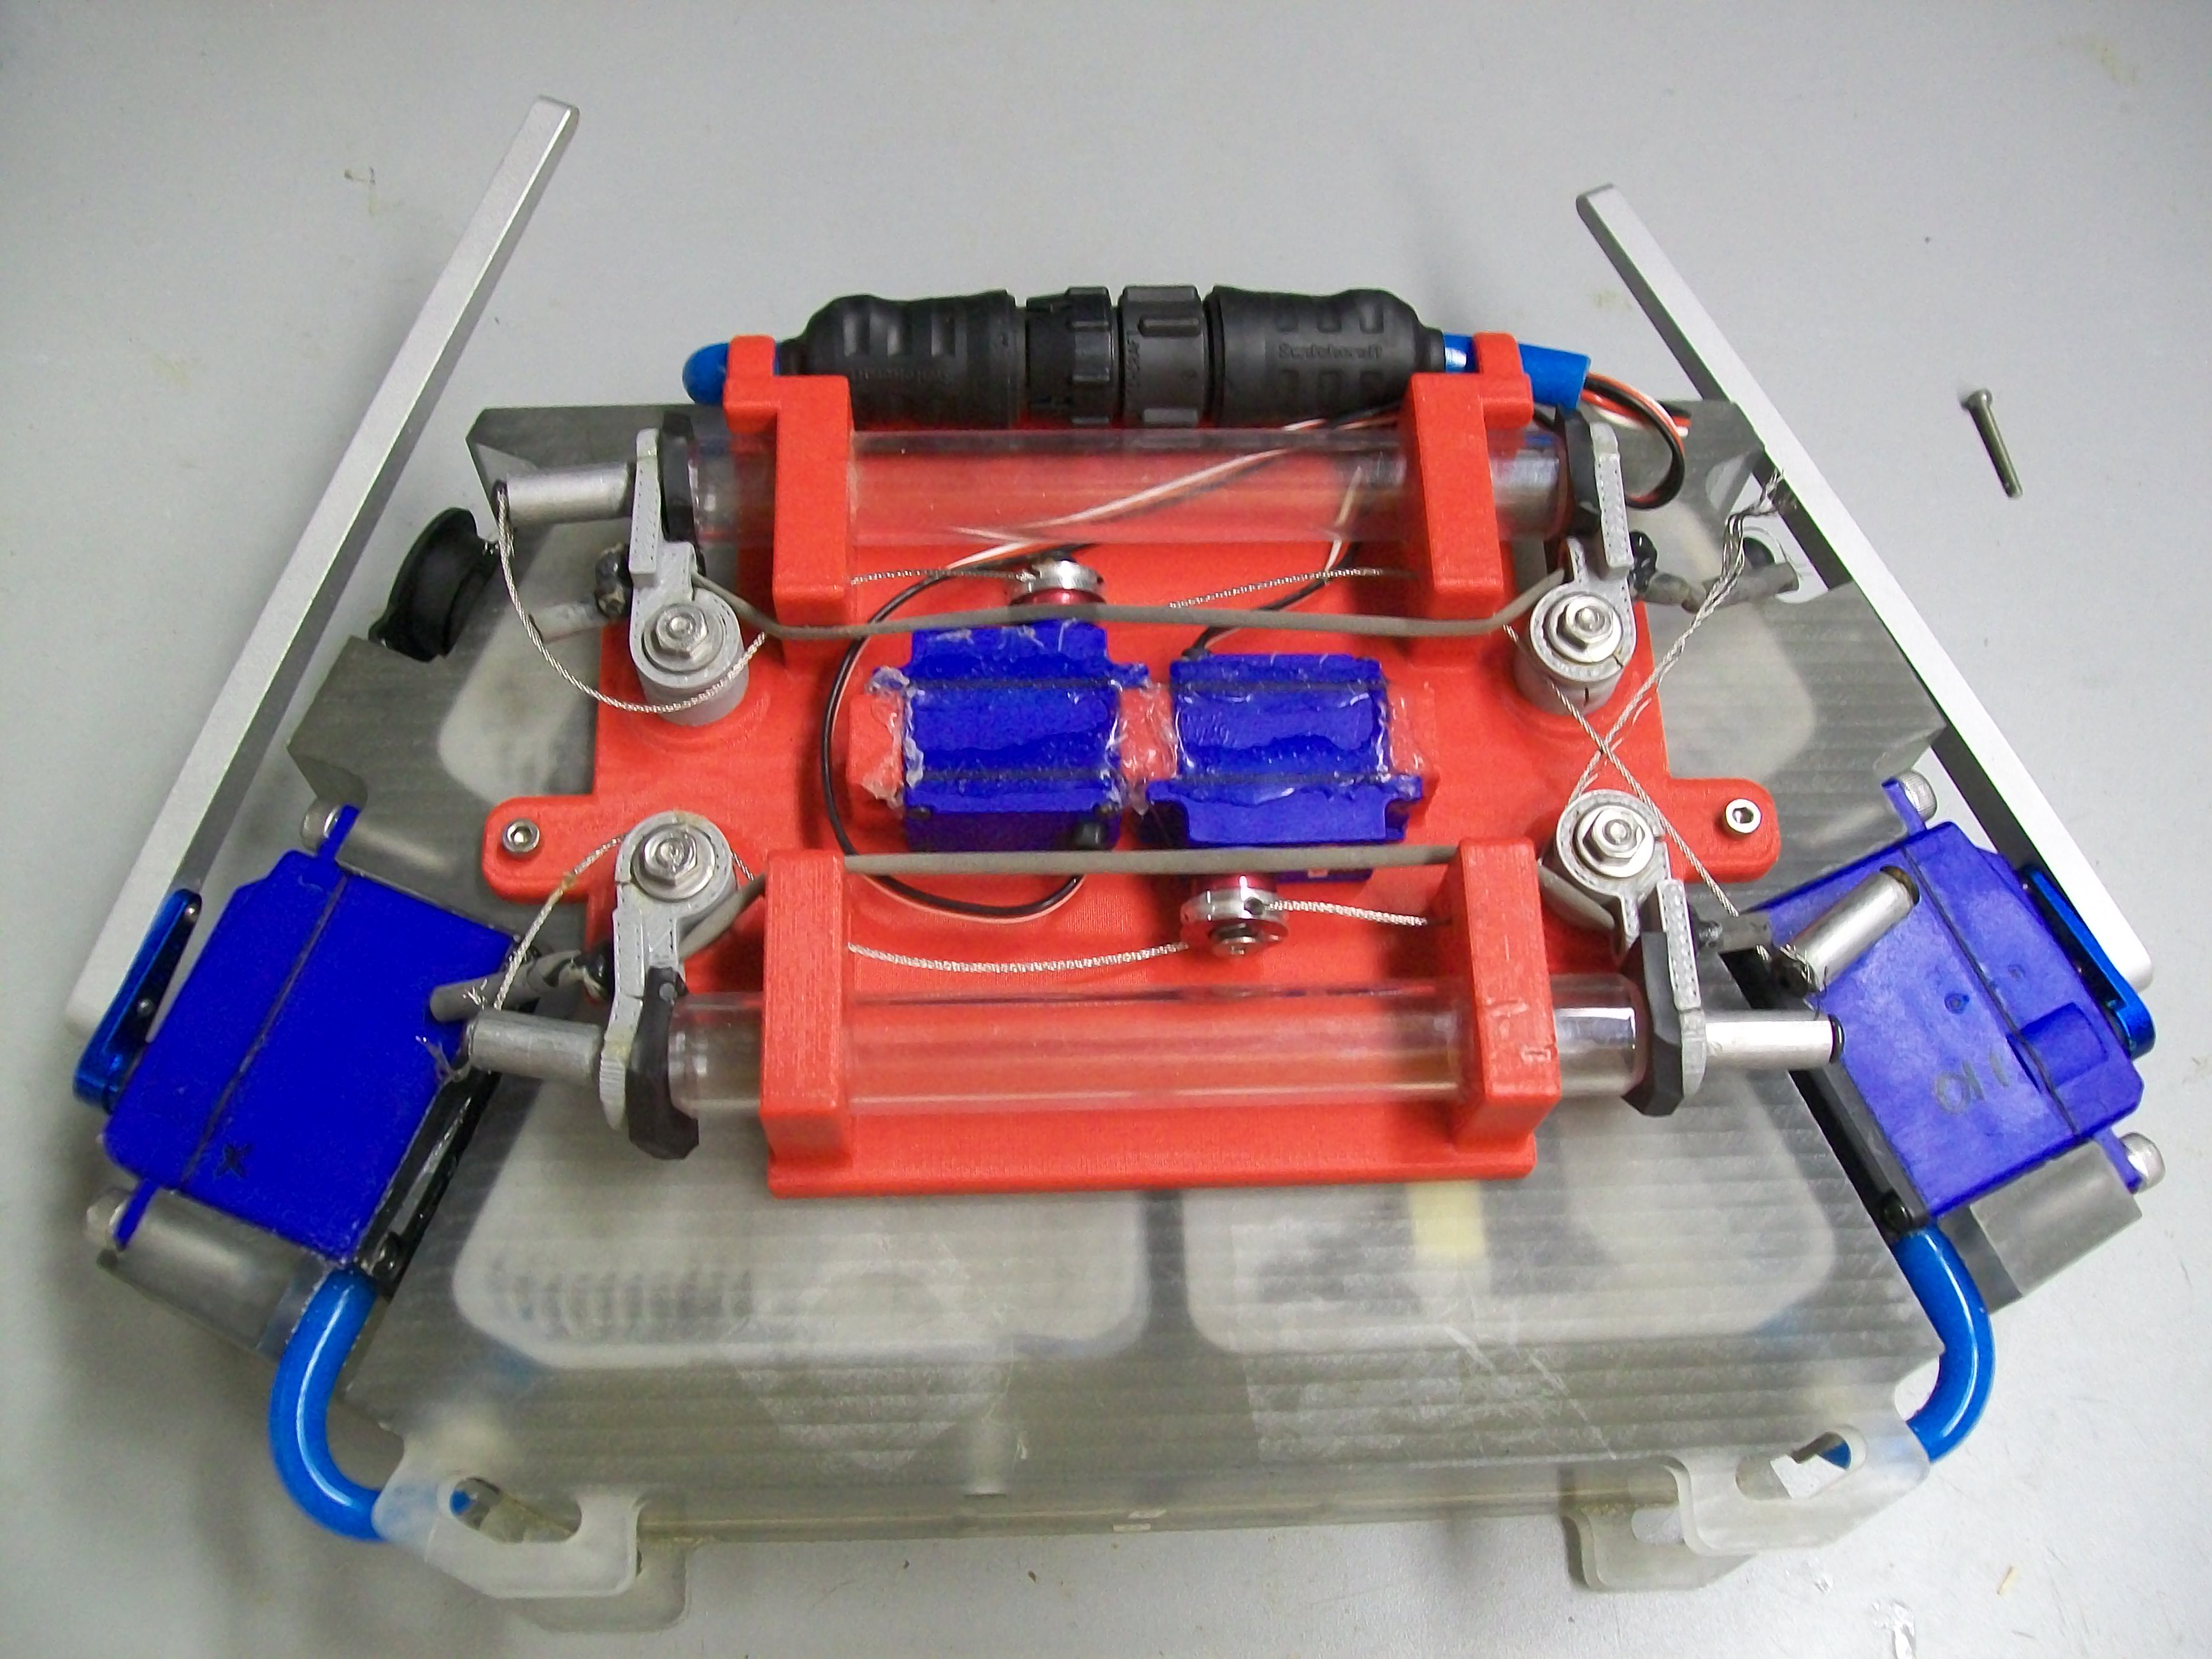
\includegraphics[width=0.9\columnwidth]{images/sampler.jpg}
		\caption{Aquapod with sampler backpack}
		\label{fig:aquapod_v1_sampler_backpack}
	\end{subfigure}
	\begin{subfigure}{0.5\textwidth}
		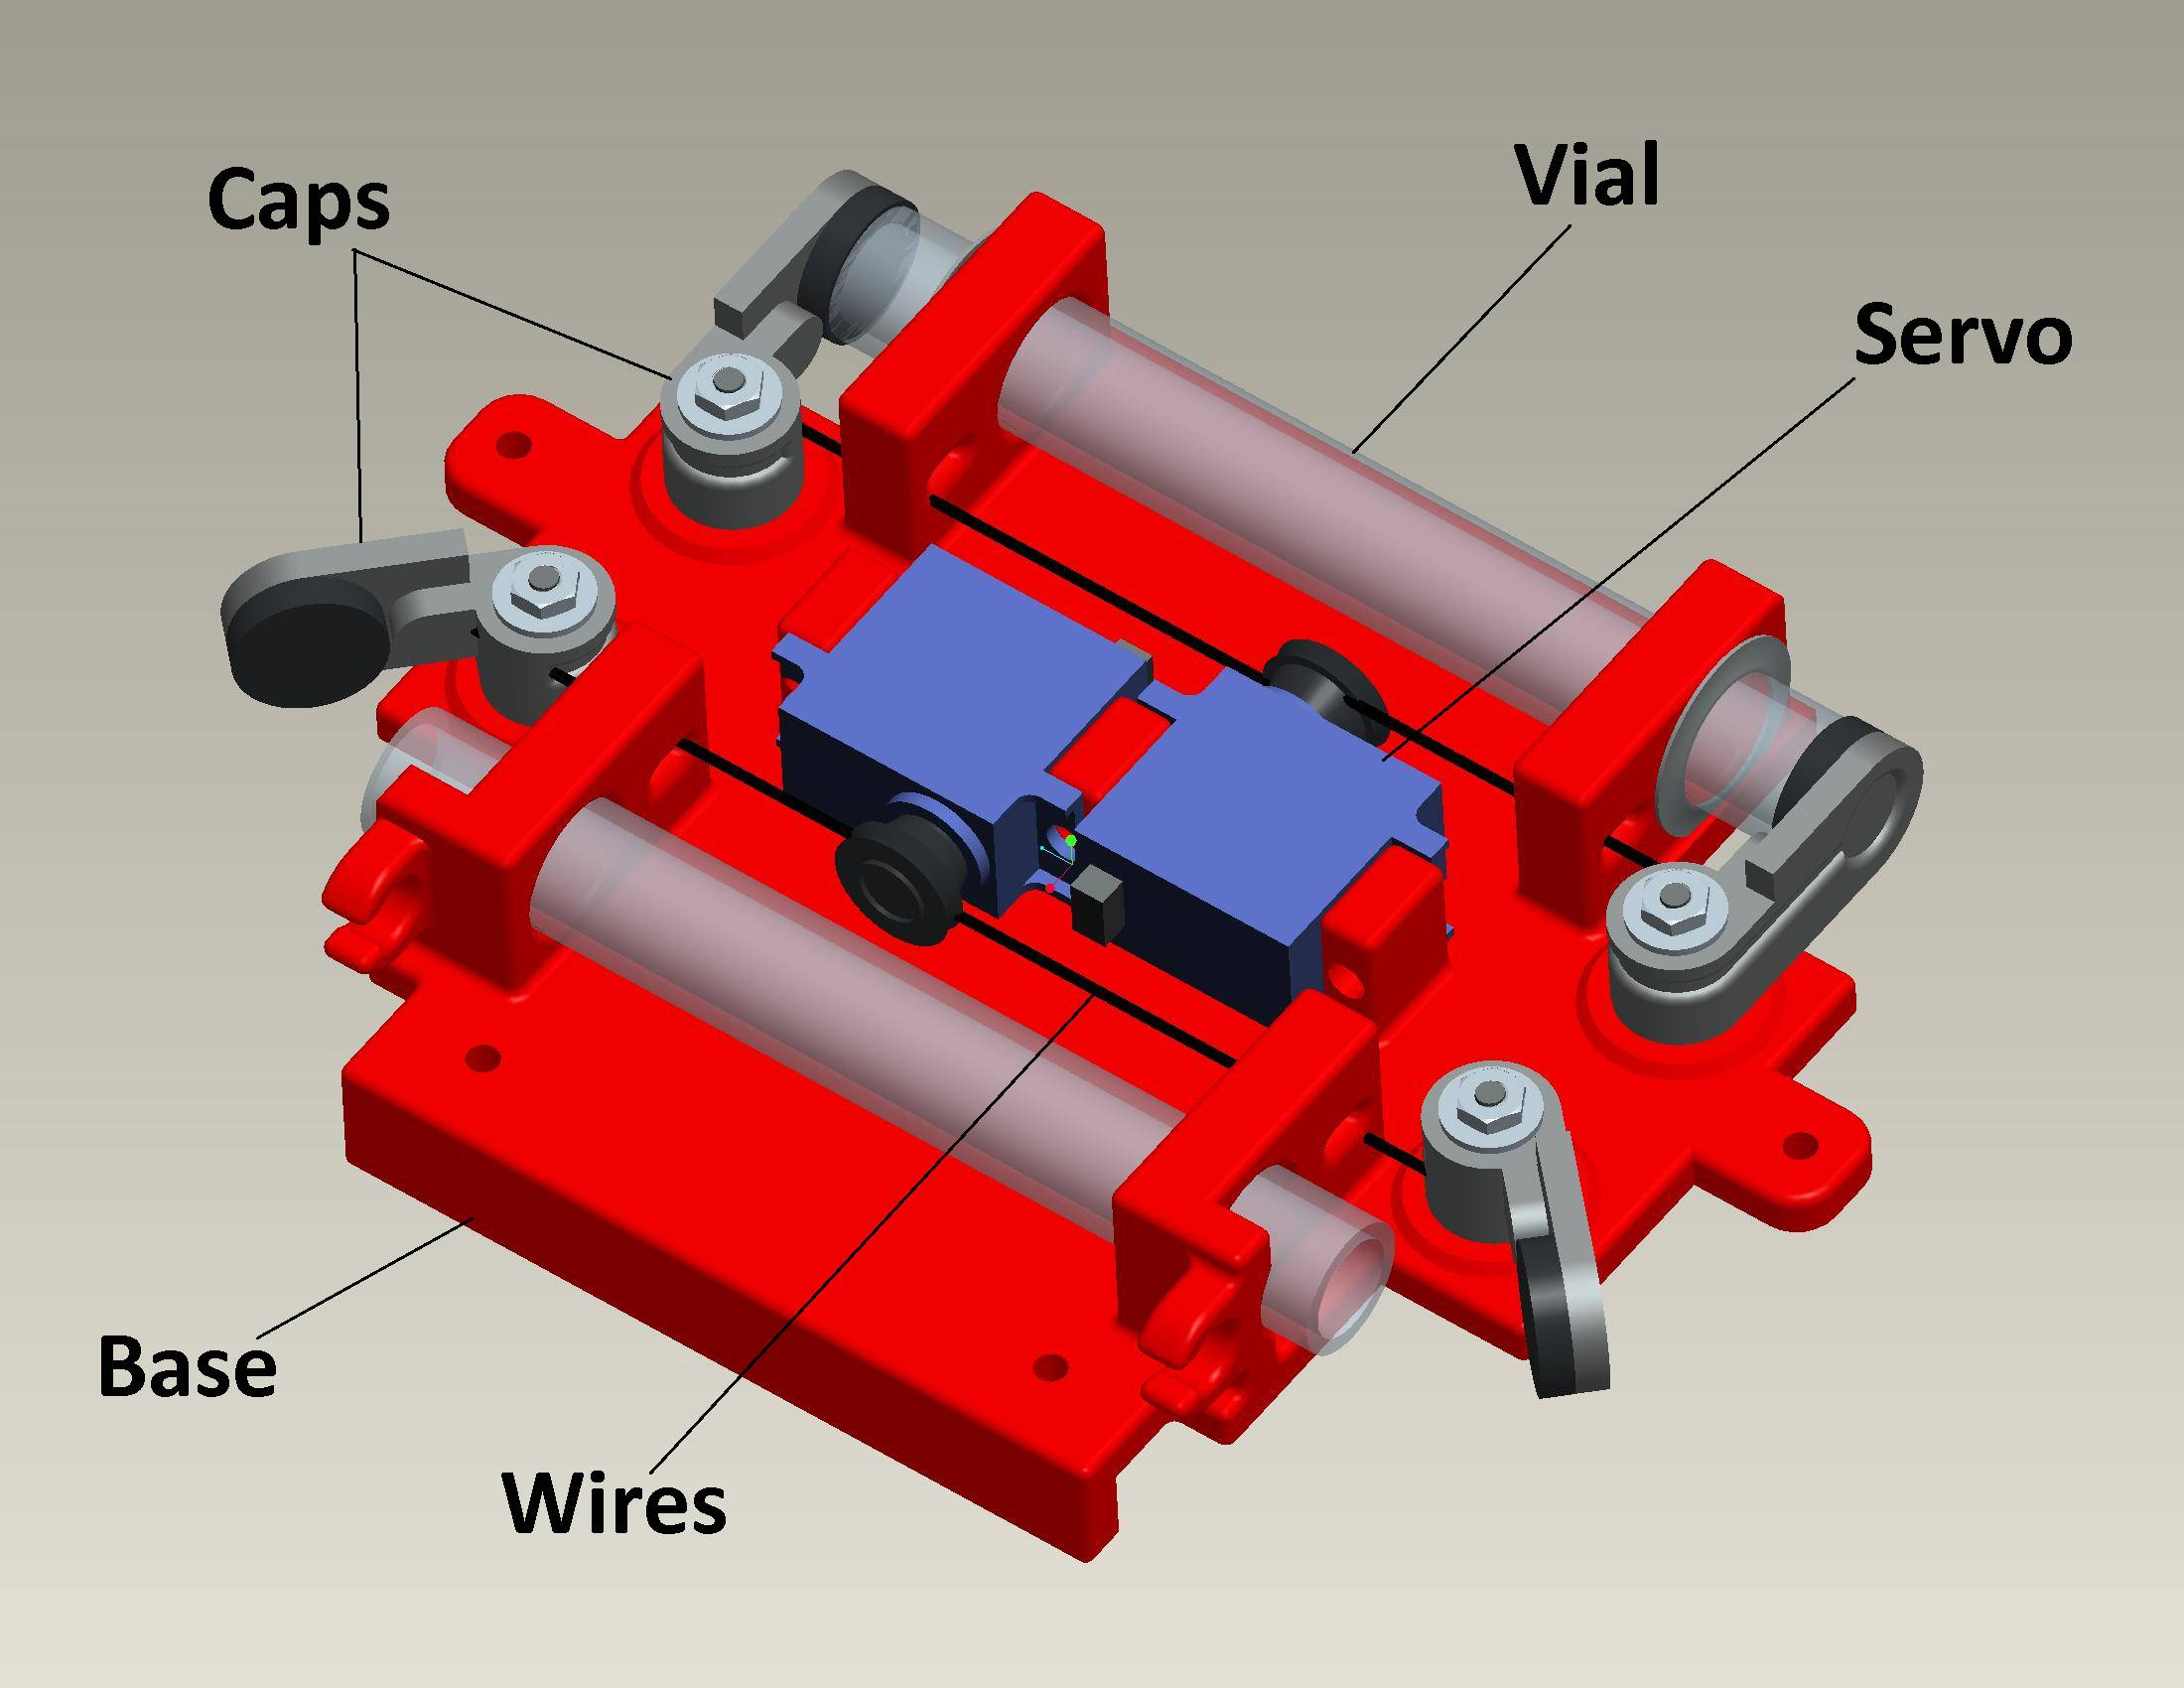
\includegraphics[width=0.9\columnwidth]{images/sampler_callout.jpg}
		\caption{Annotated sampler rendering}	
		\label{fig:sampler_annotation}
	\end{subfigure}
	\caption{Sampler on Aquapod v1 and its annotated rendering}
	\label{fig:sampler_on_aquapod}
\end{figure}

The sampler was designed based off a Van Dorn water sampler which was chosen for simplicity, lightweight, and to minimize contamination of the fluid that's sampled. There are two vials that are independently actuated by a servomotor to take samples, otherwise remaining closed with an elastic band to minimize energy use. Figure~\ref{fig:sampler_on_aquapod} shows a rendering of the sampler module which attaches to the backside of the Aquapod via screws and is connected electronically to the onboard PIC board. %A waterproof connector runs into the hull of the Aquapod to connect power and signal lines to the slave PIC board.  These connectors are also injected with epoxy to ensure a waterproof connection. 


%%%%%%%%%%%%%%%%%%%%%%%%%%%%%%%%%%%%%%%%%%%%%%%%%%%%%%%%%%%%%%%%%%%%%%%%%%%%%%%%%%%%%%%%%%%%
%\subsection{Electronic System Design}
\subsubsection{Electronic System Design}

The electronic system design was an important aspect of the Aquapod, it allowed autonomous operation to be carried while underwater, proprioceptive sensor input and logging, motor actuation, and programmability. The system consists of a master board, slave board, fuel gauge board, and sensors. The master board is an COTS Package Tracker board from Sparkfun, it communicates to the slave board via a UART interface with a custom message protocol. The slave board contains or interfaces with all of the actuators and most of the sensors, it also communicates with the fuel gauge board. The fuel gauge board is in charge of supplying the whole system with power, monitoring current usage, and charging the Lithium-ion Polymer 2-series 1-parallel battery. 

%Master board
The Package Tracker board was chosen as the master board due to time constraints and its ability to be accessed via a USB interface, allowing convenient data access and sample depth programmability via a text configuration file. The Master Board is also in charge of interfacing with the GPS unit, onboard internal temperature and humidity sensor, as well as the IMU. The state machine of the robot run on the Master Board where the inputs are values that it queries from the Slave Board. 

%This section presents an overview of the embedded system design of the Aquapod, which has been split into three main components. Two of the printed circuit boards (PCBs) were custom designed to meet the volume restrictions while the third PCB was a small, COTS module. Splitting the electronics into separate boards allows the design to be highly versatile and expand with minimal effort. This also allowed for different sensor suites to be interchanged and made the robot more robust to ever adapting needs.

%%%%%%%%%%%%%%%%%%%%%%%%%%%%%%%%%%%%%%%%%%%%%%%%%%%%%%%%%%%%%%%%%%%%%%%%%%%%%%%%%%%%%%%%%%%%
%\subsubsection{Hardware Design}
%The initial RC Aquapod had no embedded system design, and so the new iteration had to make a number of drastic changes. Due to the increase in internal components, space inside the robot was limited. A three-PCB design made up of a master board, a slave board, and a fuel-gauge board allowed the components to be broken apart and better utilize the space available. The complete system architecture can be seen in Figure \ref{fig:final-arch}.

%\begin{figure}[htc]
%finalized electrical architecture
%\begin{figure}[ht]
%	\begin{center}
%		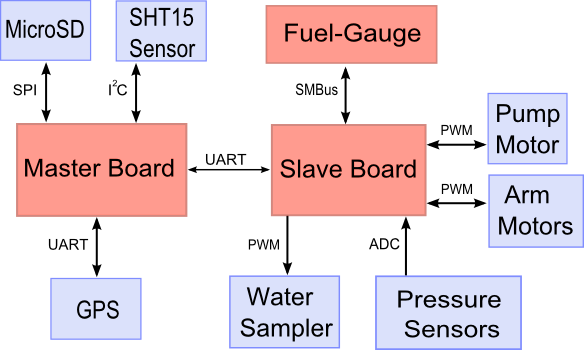
\includegraphics[width=1\columnwidth]{images/finalized-architecture2.png}
%		\caption{Final embedded system architecture}
%		\vspace{-20pt}
%		\label{fig:final-arch}
%	\end{center}
%\end{figure}

%%%%%%%%%%%%%%%%%%%%%%%%%%%%%%%%%%%%%%%%%%%%%%
%\subsubsection{Master Board}
%In order to facilitate the requirements within the time constraints, a COTS module was used for the master board. SparkFun Electronics sells this as the Package Tracker and runs on an LPC2148 ARM7 microcontroller. This unit was chosen for its 'ready to use' mircoSD card reader, onboard sensors, and GPS interface.  The master board is responsible for controlling the state machine of the robot, making decisions, and logging the sensor data.

The slave board was designed specifically to meet the demands of the Aquapod, it has a PIC16F1827 Microchip board as its main processor. It incorporates the internal pressure sensor, interfaces with the external pressure sensor, communication devices, and includes the drivers for the 5 different actuators on the robot (one for each arm motor and sampler servomotor and one for the pump motor). The slave board communicates with the Master Board and responds to its commands.   

%\subsubsection{Slave Board}

%Due to the custom nature of the hardware, the slave board was designed specifically for the Aquapod robot. The main processor was chosen as the PIC16F1827 from MicroChip based on the number of required input and output pins. The slave board also includes a pressure sensor, charge recognition circuitry, communication devices, and the required motor drivers for five separate actuators (two arms, two samplers, and one pump). This board facilitates the low-level control of the motors and sensors, however, it will only act on commands sent by the master board.

%%%%%%%%%%%%%%%%%%%%%%%%%%%%%%%%%%%%%%%%%%%%%%

%\subsubsection{Sensors}

%The Aquapod has two absolute pressure sensors with an output range of 0.3V to 4.9V, corresponding to an input range of 3 psi\(_a\) to 42 psi\(_a\), respectively. These sensors are used to monitor internal and external pressure and act as the main decision points of the state machine.


%The two arm motors feature absolute magnetic shaft encoders to report the current arm position back the slave board which handles the PID control for arm movement. The pump motor also includes a digital encoder to determine the total water volume pumped into the bladder. The sampler motors have no feedback, but operate on a standard servo open-loop signal.


%The COTS master board contains a number of onboard sensors including temperature, humidity, and a 3-axis accelerometer. The board can also access the SiRF III GPS module from USGlobalSat.


%By communicating with the slave board, the master board is capable of measuring and logging all of these sensor values in a central log file and can make decisions based on the returned values, this will be discussed in more detail below.
%%%%%%%%%%%%%%%%%%%%%%%%%%%%%%%%%%%%%%%%%%%%%%

%\subsection{Power Architecture}
The power system is comprised of the battery, fuel gauge, and charger.  The fuel gauge is in charge of charging the LiPo battery. This includes monitoring the battery's chemistry dynamics, tracking battery degradation over time, and reporting battery diagnostics to the Slave Board. 

%The Aquapods's power system comprises of three main parts: the battery and fuel-gauge, the battery charger, and the various power conversion electronics.  Wiring to chassis-mounted electronic components and high DC current lines is realized using twisted-pairs to increase noise immunity by reducing destructive (or unbalanced) effects resulting from electromagnetic interference coupled signals and ground return paths.

%\subsubsection{Battery and Fuel-Gauge}
%\label{sec:batt_mgmt_and_gg}
%At the heart of the robot's power system is a dedicated fuel-gauging chipset, described in \cite{Kottas2009}.  It provides all the necessary features to safely monitor any lithium-ion battery chemistry's dynamics, while tracking cell (capacity) degradation over time.  The resultant smart-battery system (SBS) is compliant with SBS v1.1 standards \cite{sbs_std}, and can report a wide array of static and dynamic battery parameters while idle, charging, or discharging to a host processor - in this case, the slave and master boards. This system is shown in Figure \ref{fig:pwr_blk_diag}.

%A lithium-ion polymer battery (LiPB) was chosen to power the robot.  This particular battery chemistry was selected due to its thin and light-weight packaging, high energy density and output power capabilities.  It can source roughly 14Wh of energy, and satisfies the robot's operating time requirements. 

%A highly integrated LiPB switch-mode charge-management circuit is included on slave board.  It is configured to charge the LiPB pack quickly and safely and contains a pre-charge (conditioning) mode for deeply discharged batteries.

%\begin{figure}%
%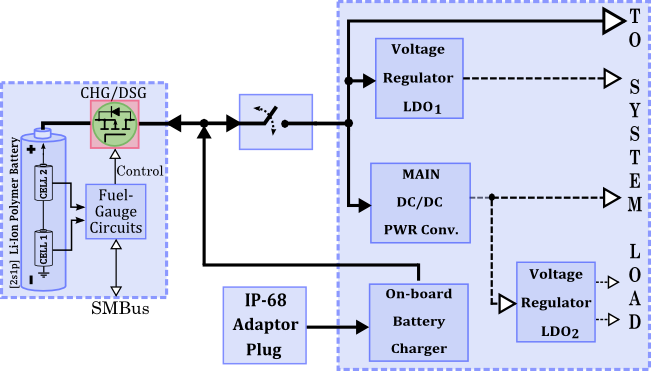
\includegraphics[width=1\columnwidth]{images/Aqua-Pod_Robot_PwrSys_Fig01.png}%
%\caption{High-level power system block diagram}%
%\vspace{-10pt}
%\label{fig:pwr_blk_diag}%
%\end{figure}

%%%%%%%%%%%%%%%%%%%%%%%%%%%%%%%%%%%%%%%%%%%%%%
%\subsubsection{Communication Protocol}
%Command and Acknowledgment (CMD/ACK) messages are used to exchange data and commands between the boards. This hand-shaking protocol was enforced to ensure important commands from the master board were being process and executed by the slave board before continuing with the state machine. The master board can send one command at a time in a 9-byte packet to the slave board which will execute the command or return sensor values appropriately.  
%%%%%%%%%%%%%%%%%%%%%%%%%%%%%%%%%%%%%%%%%%%%%%
\subsubsection{State Machine and Operational Profiles}
The main purpose of the Aquapod was to allow diving and surfacing autonomously in a body of water taking measurements along the depth profile. The information gathered would then be analyzed by a biologist to identify interesting depth location and then two independent depths could be programmed for liquid sampling. 

A state machine was implemented to cycle through the different modes states available: an instant dive mode, a remote controlled triggered dive, land mode for remote control land locomotion, and bladder expulsion to expel residual bladder fluid. 

%The main purpose for this version of the Aquapod was to collect water samples at a pre-programmed depth. Using a graphical user interface, the Aquapod can be programmed into one of four modes, including: Instant Dive(1), Remote Dive(2), Land Mode(3), and Purge Bladder(4). Selecting one of these modes will route the robot through the state machine which can be seen in Figure \ref{fig:Statemachine}.

%\begin{figure}
	%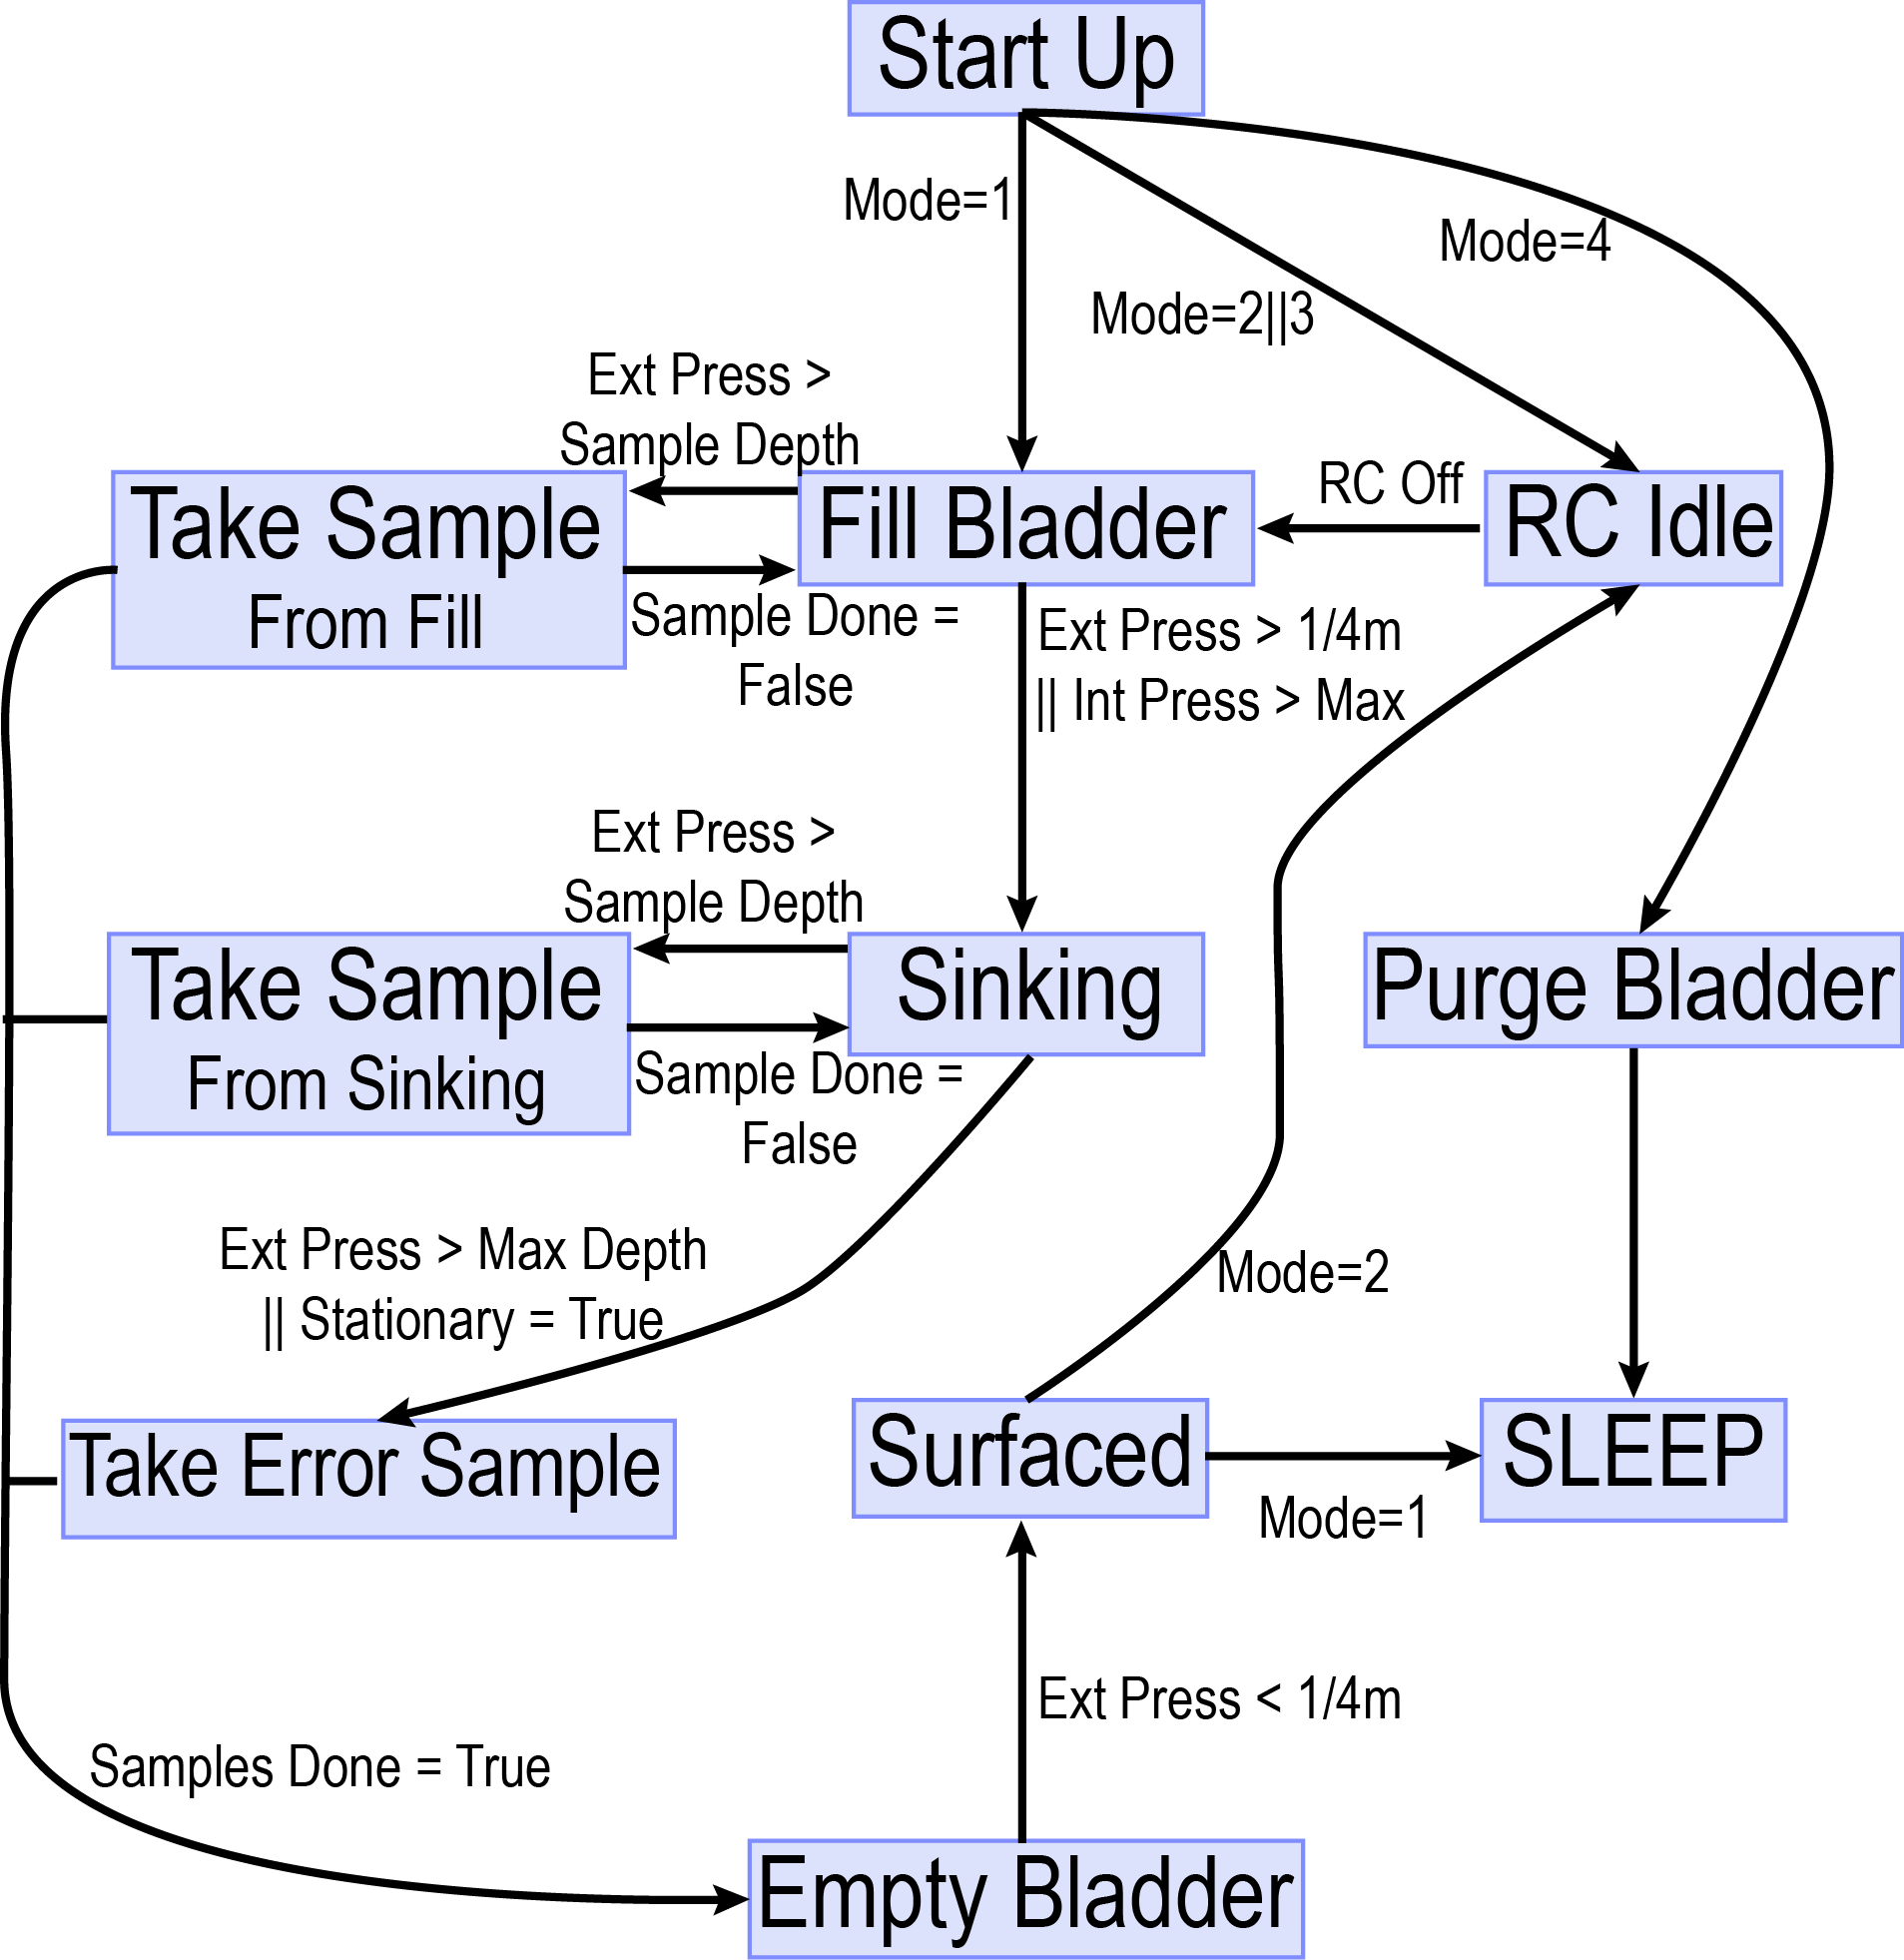
\includegraphics[width=1\columnwidth]{images/Statemachine.png}
	%\caption{Aquapod state machine diagram}
	%\vspace{-10pt}
	%\label{fig:Statemachine}
%\end{figure}

%It was important to program a number of safety checks within the state machine to ensure that the robot will always resurface. Errors in the operation could include reaching a depth greater than 10m or hitting a surface before reaching the target depth. If one of these errors occurs, the robot will take a sample and return to the surface. Other system error checks were written directly into the slave board in case one of the boards reset, a sensor failure occurs, or other unlikely mishaps happen.

%During either mode 2 or 3, the remote control (RC) operation is run. This allows the user to control the arms of the robot through a standard radio transmitter. In these modes the user can command the robot to tumbling to a particular location and dive or simply move around on land.


%The state machine featured in Figure \ref{fig:Statemachine} is by no means extensive of the robot's capabilities. Further development and inclusion of the GPS module can greatly increase the functionality of the robot. This operation profile was simply used as an example for diving/sampling and as a demonstration tool. Autonomous control for long-term and unmonitored missions is feasible with the current hardware.

%%%%%%%%%%%%%%%%%%%%%%%%%%%%%%%%%%%%%%%%%%%%%%%%%%%%%%%%%%%%%%%%%%%%%%%%%%%%%%%%%%%%%%%%%%%%
%\subsection{Experiments}
%\label{experiments_aquapod}
%To verify the mechanical design and embedded system programming, numerous experiments were carried out in a diving well. Figure \ref{fig:logfile} shows the results from a sample dive that was taken. The robot was programmed to take samples at 1m and 3m. The output log file includes the internal pressure values, depth in meters, the accelerometer sensors, temperature, and humidity. Markers are placed on the pressure graph to indicate event locations either the pump turning on or off(solid), or when a sample was taken(dotted).

%Pressure log file 
%\begin{figure}[htb]
	%\centering
	%\includegraphics[width=1\columnwidth]{images/testresults.png}
	%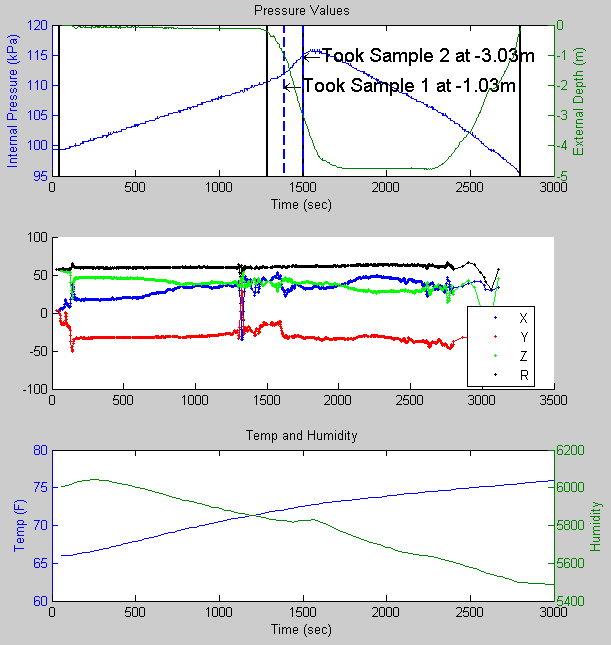
\includegraphics[width=1\columnwidth]{images/logfile.png}
	%\caption{Experiment log file from an Aquapod dive}
	%\vspace{-10pt}
	%\label{fig:logfile}
%\end{figure}

%In addition to in-lab testing, the Aquapods were also brought to Houston for user testing with research biologists. The robots were demonstrated in several locations in marshlands near the coast including heavily vegetated and muddy environments. Feedback from this visit will be taken into consideration for future iterations of the Aquapod family.

%%%%%%%%%%%%%%%%%%%%%%%%%%%%%%%%%%%%%%%%%%%%%%%%%%%%%%%%%%%%%%%%%%%%%%%%%%%%%%%%%%%%%%%%%%%%
%\subsection{Future Work}%
%\label{future_work}
%Though this iteration was a major improvement in functionality over the pervious RC Aquapod, many improvements are continously being explored to expand its capabilities. One area of continuing work for the Aquapod is communications. Currently the only method of communication is through hobby RC signals. However, Aquapods can be configured to carry distinct communication payloads, with each Aquapod serving as a node in a network that enables digital radio, cellular, and acoustic communications. 

%Improvements to the electrical power system design include the use a single-cell LiPB. This broadens the range of compatible input power sources to include various energy harvesting modules - such as solar, wave, thermal, kinetic, etc.  Integrating dynamic power-path management into the charging circuit, in tandem with energy harvesting may also increase efficiency of energy use achieving overall gains in the robot's achievable runtime.

%Another improvement relates to using the Aquapod for extended-period environmental monitoring. In this scenario, the robot collects relevant data in a manner that minimizes energy consumption for periods of 12 to 24 hours and then navigates to a waypoint for pickup.


%%%%%%%%%%%%%%%%%%%%%%%%%%%%%%%%%%%%%%%%%%%%%%%%%%%%%%%%%
\subsubsection{ Conclusions}

The combination of the high terrainability, high mobility-to-size ratio, amphibious nature, and small size allows the deployment of the Aquapod in environments that would be difficult for most robots of the same size. The robot is designed to withstand water pressures up to 10 meters in depth, as well as be chemically compatible with the potential substances it may encounter.  The onboard embedded system was designed to perform as many modular expandable tasks in a limited amount of space, as well as provide intelligent power management to the system.  The redesign and further development of this robotic platform provided several advances in its capability for the specified environment of a shallow water marshland.

%\clearpage
\subsection{Screwdrive Propulsion System}
\label{sec:screwdrive}

% Screwdrive locomotion subsection 
% Screwdrive images: https://docs.google.com/drawings/d/1YzuIb8U-4fQxipOJEBA4PD4eBe6fdJJcrUts8n2fkNc/edit 

\begin{figure}[!htb]
	\begin{subfigure}[t]{0.5\textwidth}
		\centering
		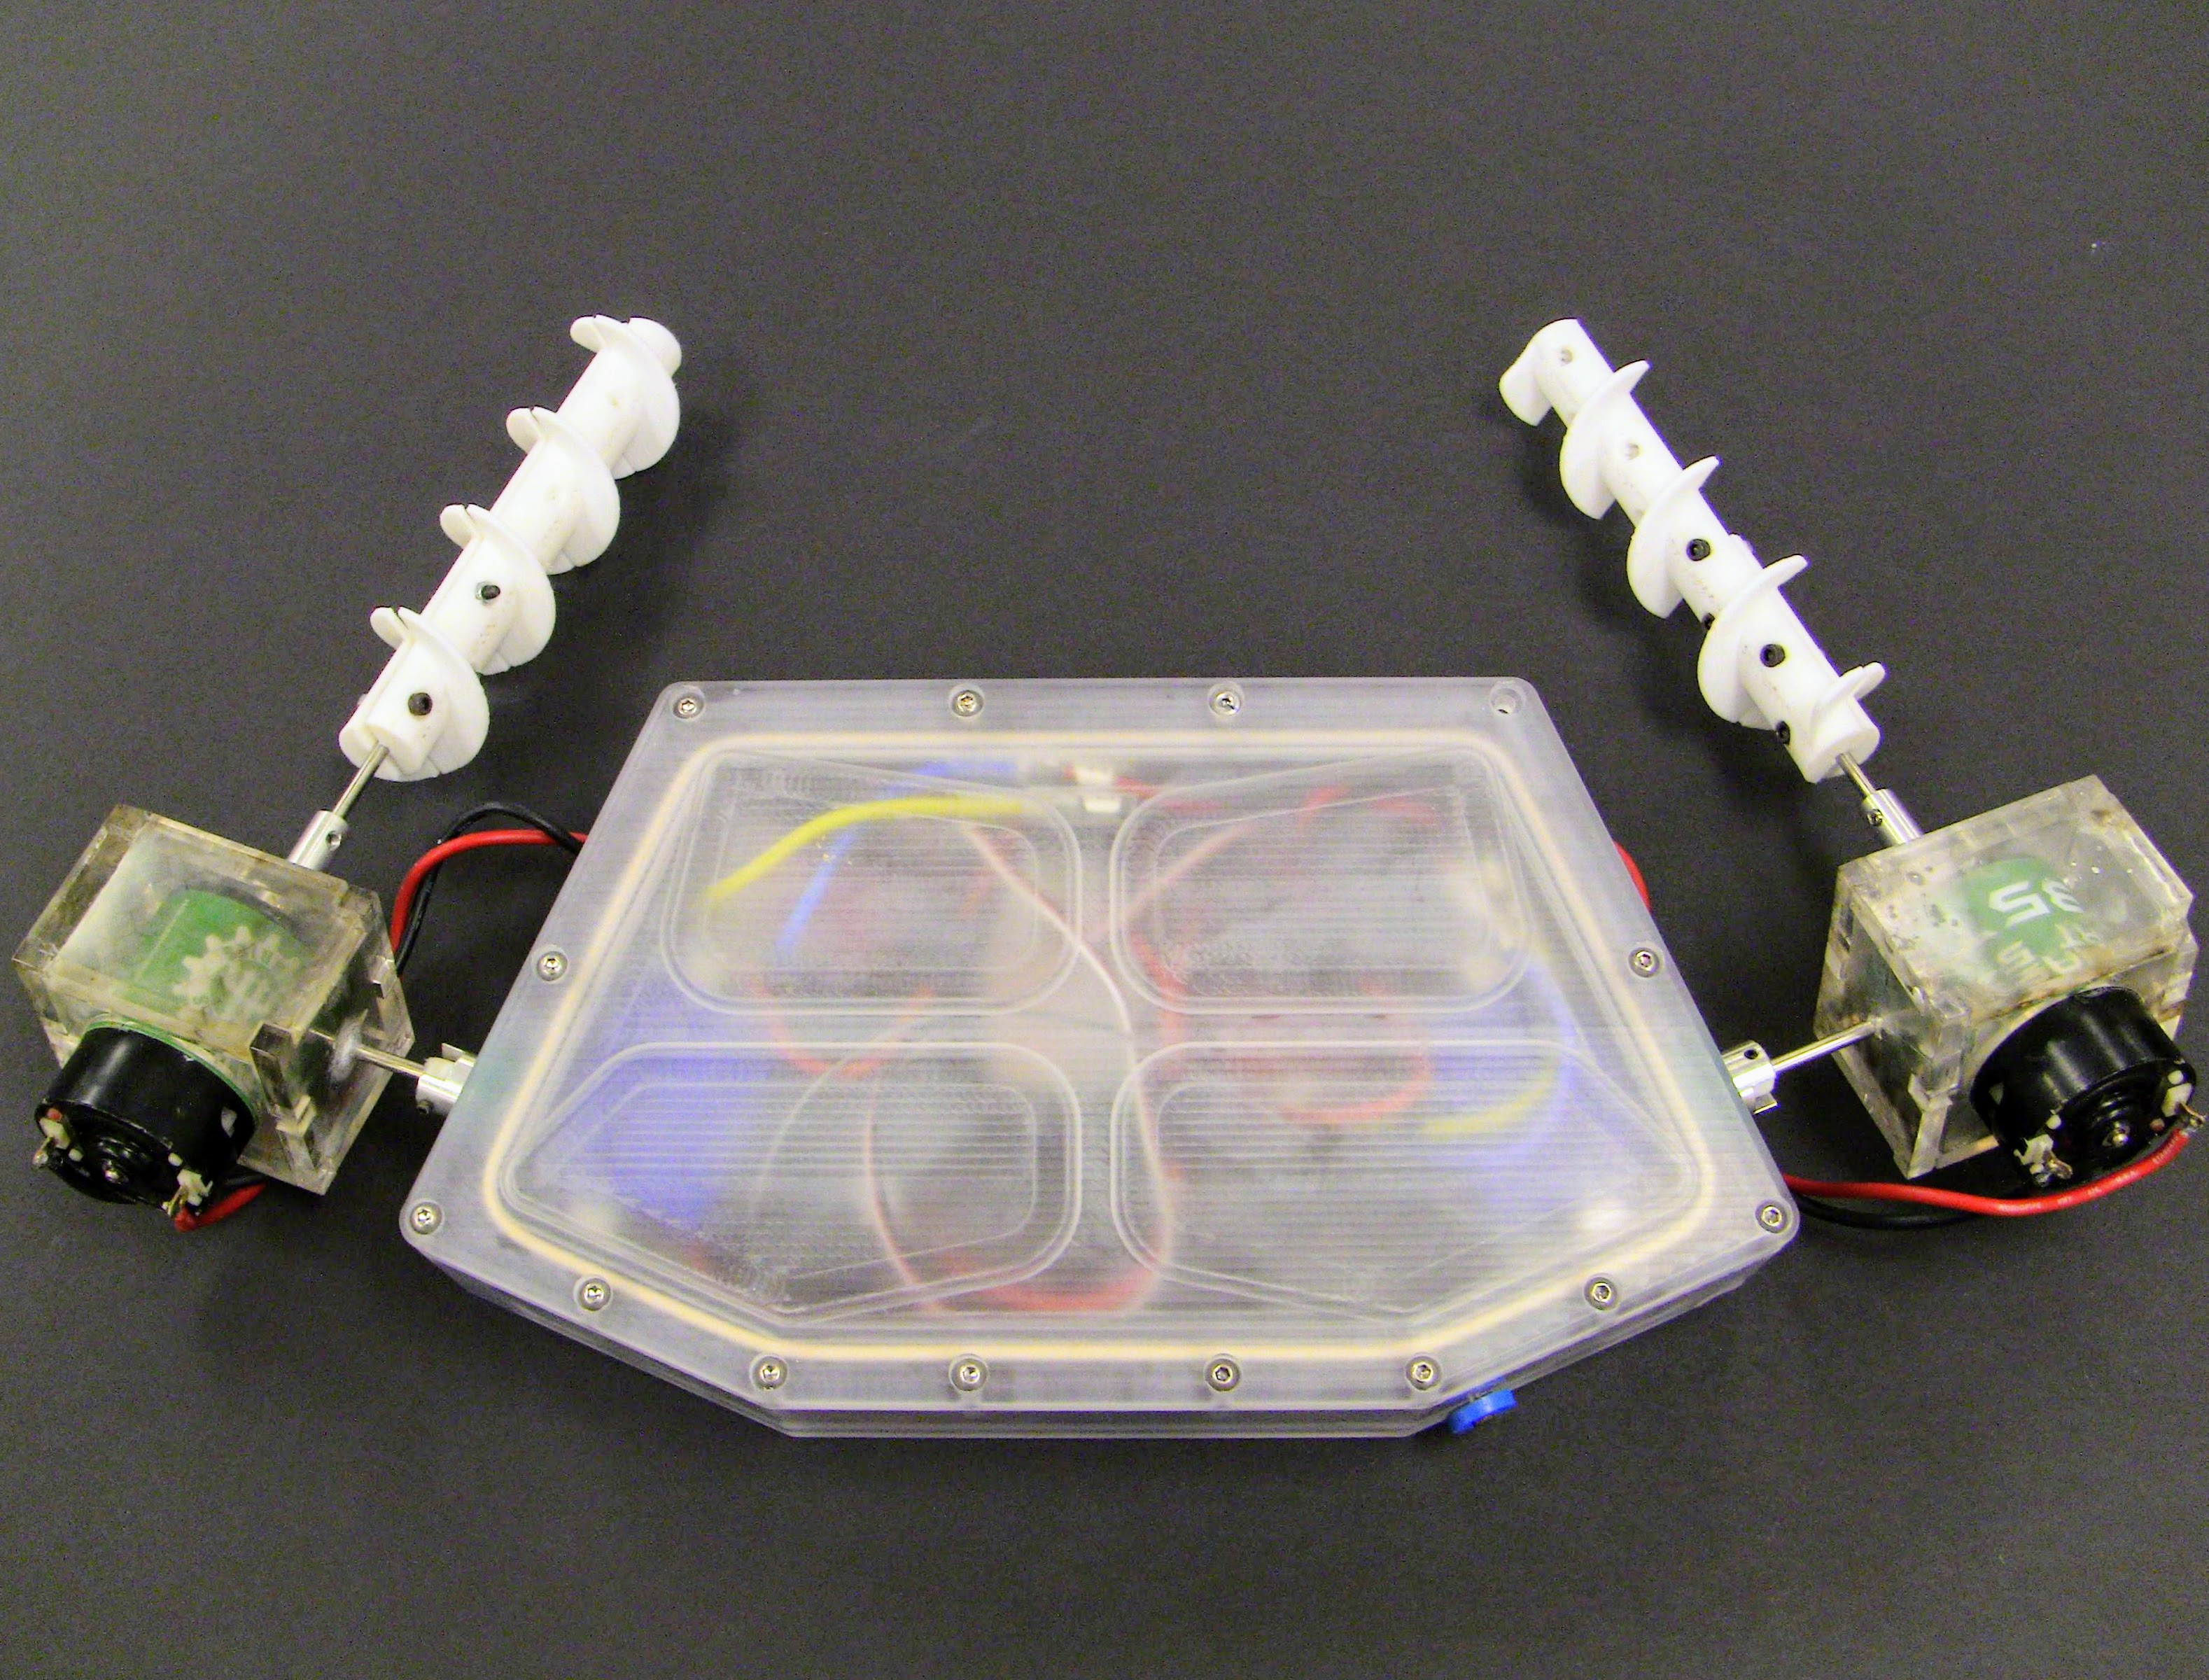
\includegraphics[width=\linewidth]{images/aquapod_v2_screwdrive.jpg}
		\caption{The dual screwdrive arms on the Aquapod}
		\label{fig:screwdrive_aquapod}
	\end{subfigure}
	\begin{subfigure}[t]{0.5\textwidth}
		\centering
		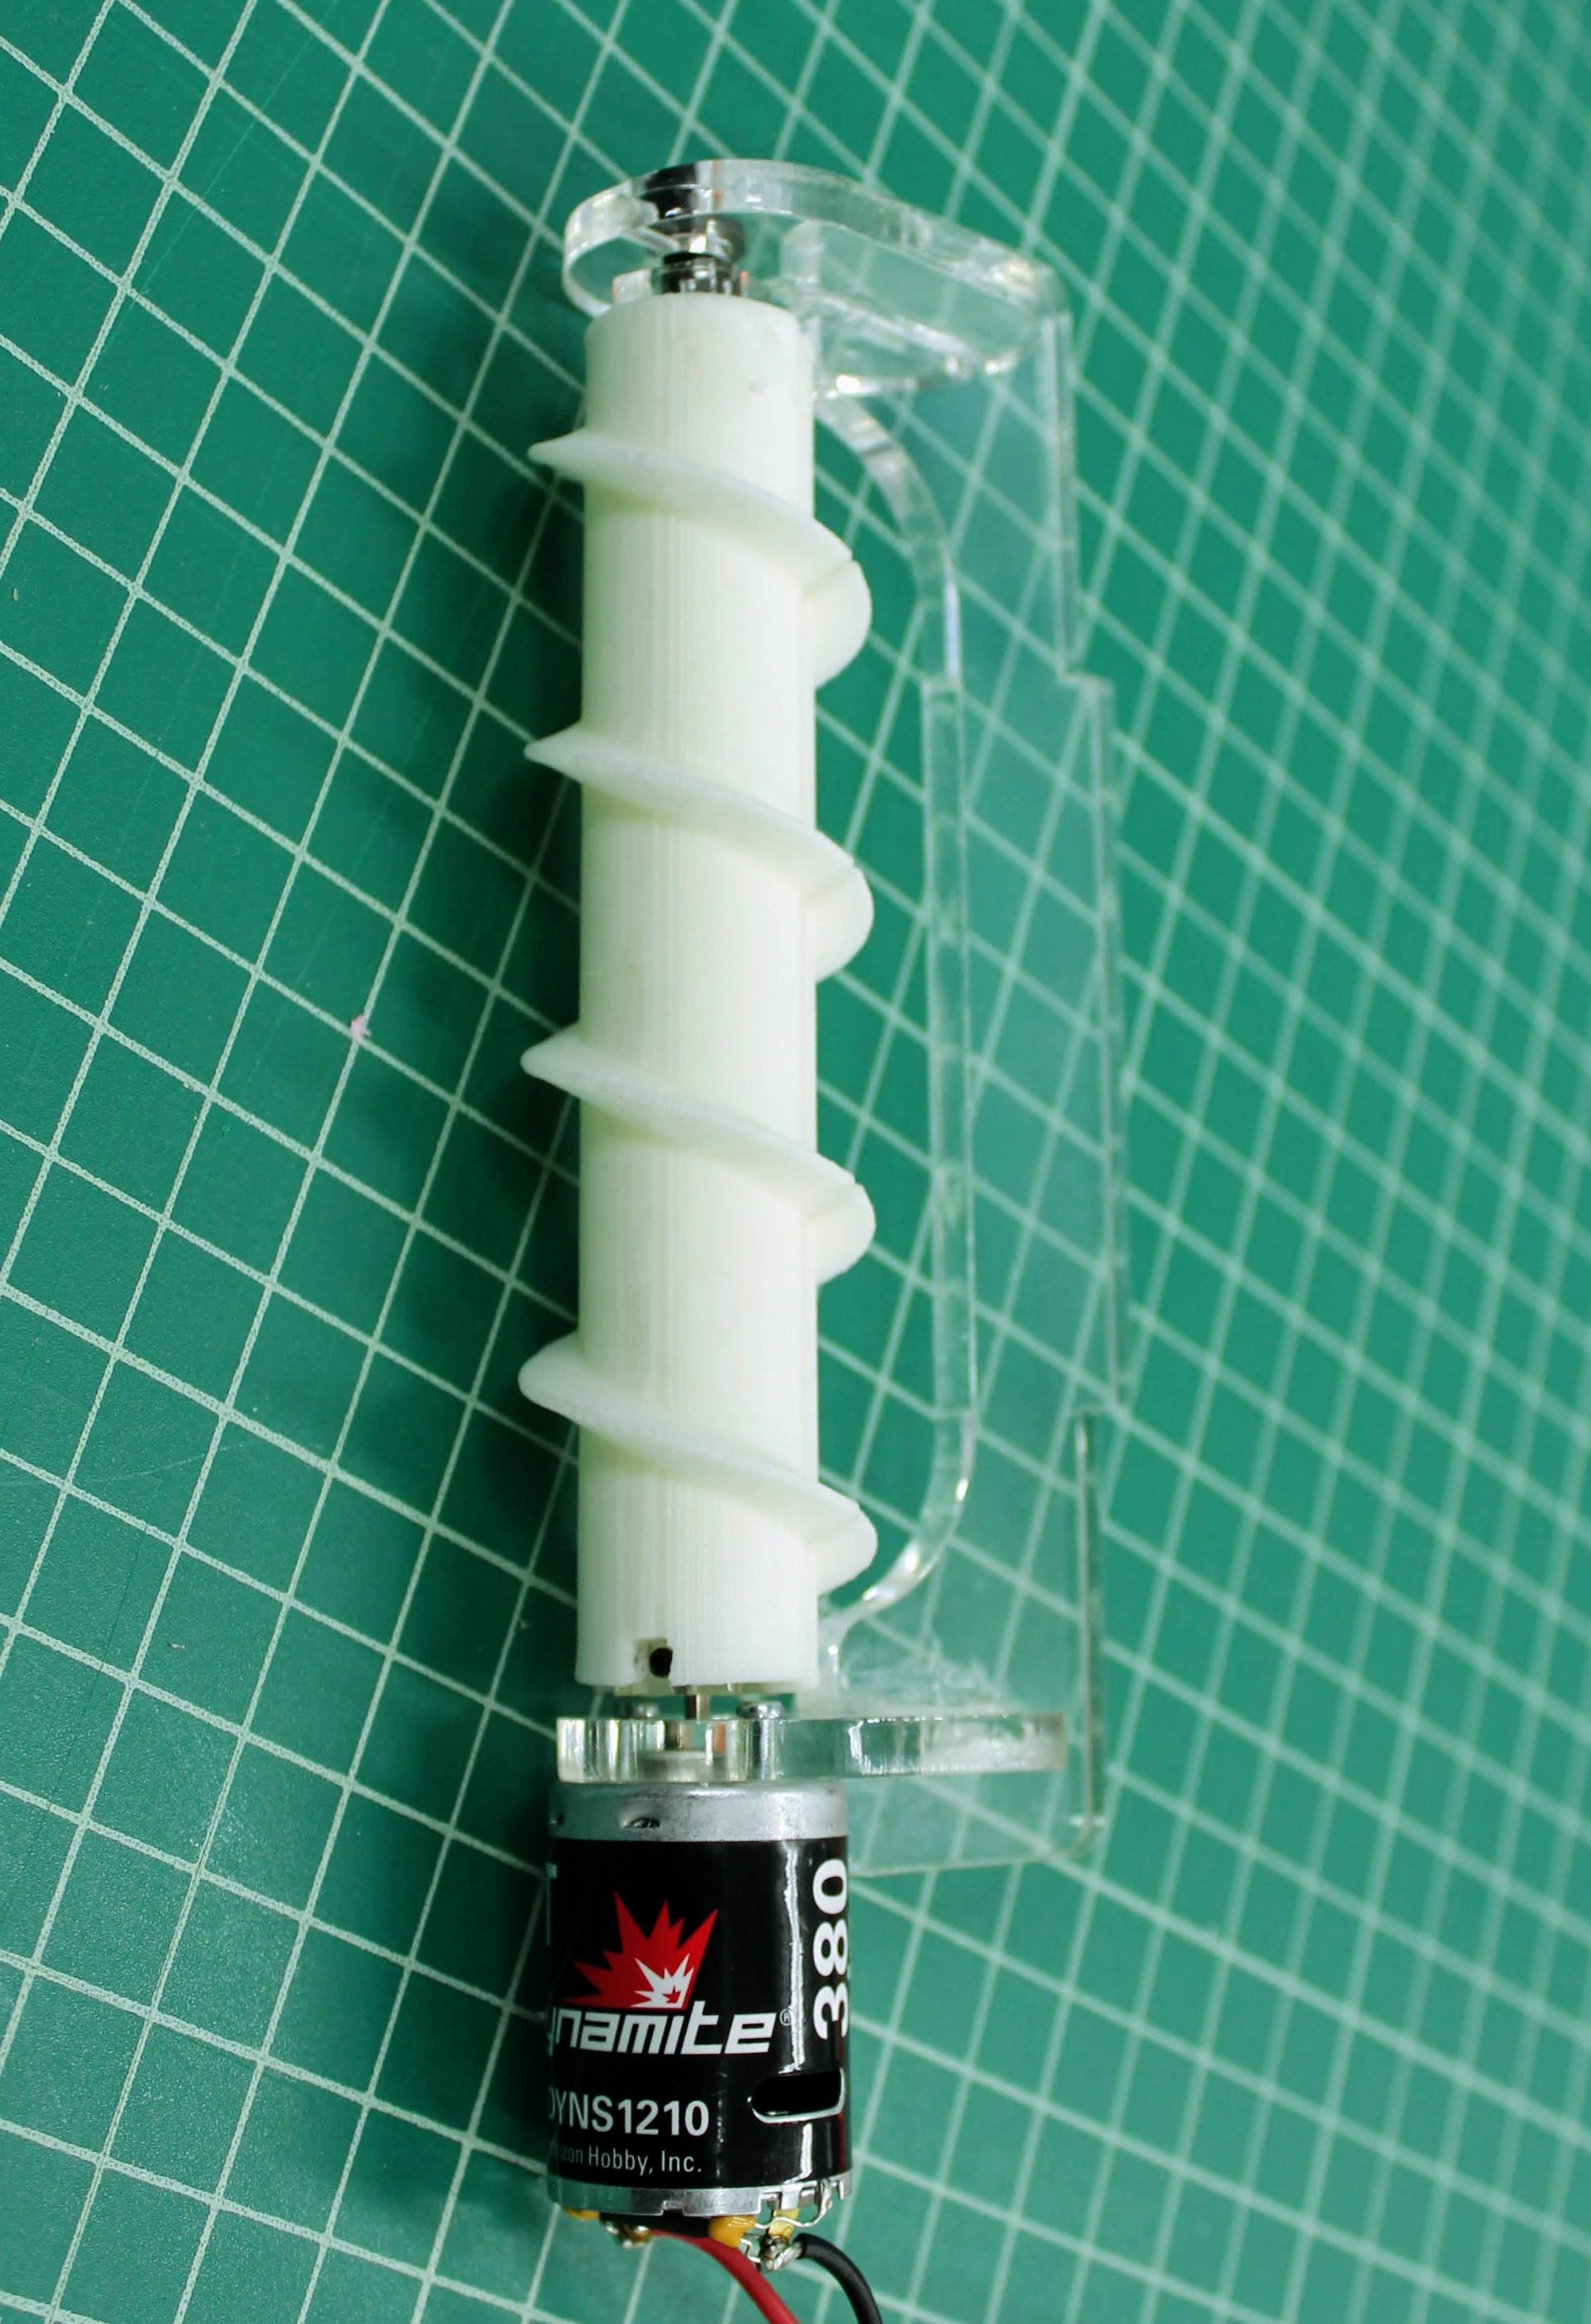
\includegraphics[width=0.5\columnwidth]{images/sd/screwdrive_omnibot_screw.JPG}
		\caption{Prototype screw}
		\label{fig:screwdrive_omnibot_screw} 
	\end{subfigure}
	\caption{Screwdrive screw prototypes}
	\label{fig:screwdrive_screw_prototypes}
\end{figure}

% why 
The motivation for research into amphibious modes of locomotion was born of two factors. One, to develop a suitable mode of locomotion for the amphibious Aquapod that could work on land, water, and terrains in between. Two, to complement tumbling locomotion with an alternative that would allow controllable steering. Steering would in turn permit motion planning as well as optimal obstacle approach for tumbling.

To complement tumbling and solve the controllability problem, the treaded Adelopod \cite{Hemes2011a} utilized a set of tank-like treads driven independently by DC motors to create a differential drive. This addition enabled predictable and more energy efficient motion control while using the original tumbling capability to overcome obstacles. While treads work well on land and surface water operation \cite{Kline2012}, they do not work well underwater. 

%Additionally, corner cases where the Adelopod could become stuck, due to legs or body jamming against the terrain, could now be overcome with the treaded drive in conjunction with arm actuation. 

%While treaded locomotion proved to be an inexpensive and simple solution to complement to tumbling on land, tread drives do not work well while completely submerged in water. Treaded drives have been used \cite{Kline2012} in amphibious applications albeit for surface vessels. Treads work in a manner similar to a paddleboat's wheel where propulsion is generated by the paddle pushing against water as it rotates. However, in a wheel, as with any cyclical system, as one paddle pushes in one direction, there is another paddle that provides propulsion of the same magnitude and opposite direction, resulting in no net propulsion. 

%Treaded systems work when only partially submerged as one side of the treads pushes against water and the other against air, resulting in net propulsion.

There exist many methods to provide actuation that range from the most simple flagellum-type propulsion mechanisms \cite{Regnier2014,Dhariwal2004, Edd2003}, to fish-like propulsion \cite{Yu2018,Massey1984}, and others such as anguilliform swimming \cite{Zhou2011}, however, with the exception of anguilliform locomotion, these methods do not work well or at all on land. %Could add bit about amphibious platforms here before diving into the DARPA amphibious vehicle. 

%DARPA's most recent attempt into amphibious locomotion consists of a vehicle used in a logistics-enabling role, moving supplies from boats towards the shore. This vehicle, named the Captive Air Amphibious Transport (CAAT) \cite{Kline2012}, uses buoyant pontoons together with treads to move on the water's surface, then transitions to land and operates as a tank would. 

In the 1960s, the predecessor of DARPA, the Advance Research Projects Agency (ARPA) along with other government agencies funded research into another form of amphibious locomotion: \emph{the screwdrive}. This is a relatively neglected method of locomotion that has been shown to successfully propel military, scientific, and recreational vehicles across a wide variety of terrains ranging from snow to water and mud to sand \cite{Fales1972, Cole1961, Dugoff1967}. This method of locomotion can trace its roots back to 1804 when Colonol John Stevens took the Archimedes screw concept and applied it to drive a steamboat on New York's North River \cite{Dugoff1967}. Screws then found use in land-based applications in the form of the Fordson tractor \cite{Freeberg2010} in the 1920s. There was a proposal in 1948 for a screw-propelled amphibious vehicle in England \cite{Cole1961}. %Additionally in 1957 a German firm also demonstrated a screw-propelled amphibious vehicle during the Hanover Exhibition. The USSR found use for screw-driven vehicles to retrieve space cosmonauts from terrains consisting of deep snow \cite{Freeberg2010}. 

% research timeline
%Most of the available research into screwdrive locomotion and its design parameters dates back to the 1960s and 1970s when Dr. Cole \cite{Cole1961}, of the University of Birmingham in England, and the Chrysler Defense Corporation \cite{Fales1972, Dugoff1967}, through US Military funding, carried out research in this method of locomotion for littoral environments. Recently, Freeberg et at. \cite{Freeberg2010} conducted research on quad-screw configuations and compared its performance relative to the traditional dual-screw. Nagaoka et al. \cite{Nagaoka2011} have explored the modeling of a dual screw system in compliant terrain, specifically moon soil, or regolith. %Both Freeberg and Nagaoka studied the peculiar maneuverability charecteristics of screwdrive systems as these are relatively unexplored compared to traditional locomotion methods. In the field of robotics, screwdrive propulsion is not common, however, it presents a mechanically-simple, robust, inexpensive, and multi-domain method of locomotion. 

% TODO: update to reflect current structure 
The following section will focus on the parameters that define functional characteristics of screwdrives. The next section covers the particular maneuverability properties of screwdrive systems. Finally, proposed research on screwdrive systems is covered in the last section. 


%\subsubsection{commented out text }
%The U.S. military started research on the screwdrive by retrofitting a Weasel tank with screws. Formal research on the parameters of screw propulsion didn't start until the 1960s with Chrysler Defense Corporation \cite{Dugoff1967} \cite{Kress1965} and Dr. B.N. Cole in England \cite{Cole1961}. These two research initiatives form the bulk of known research into this form of locomotion. That being said, screwdrive locomotion has been used for mining applications such as the Mudmaster, the Snowbird platforms which were used in attempts and ultimate success crossing the Bering Strait, the Spiral Track Autonomous Robot of Lawrence Livermore National Laboratory \cite{Perez1996}, and the Tyco Terrain Twister toy remote controlled vehicle.

%The above mentioned applications had various things in common. Terrains that were found to be best for screw-propelled locomotion, herein referred to as screwdrive locomotion, were terrains that were marshy, snowy, or icy. Much like the Aquapod, for exclusively moving on water or land domains, there are better ways locomote. Another commonality is that, excluding the Terrain Twister, all vehicles above employed dual parallel screws for lomotion. A notable exception is the Terrain Twister that uses an additional actuator to alter the angle between the screws, similar to the Adelopod \cite{Hemes2011}. Freeberg \cite{Freeberg2010} explored and compared different screw configurations against the conventional dual screw design. 

%An important characteristic of screwdrive locomotion is that it is highly dependent on the terrain in which it operates, as described in \cite{Cole1961}, \cite{Kress1965}, \cite{Dugoff1967}. This presents both an opportunity and a challenge. It's a challenge in the vehicle model will necessarily then depend on the terrain, this is because the screw blade must be able to cut into the medium in order to create forward travel \cite{Freeberg2010}. Dual systems are typically oriented parallel to the longitudinal axis of the body, and if the blade is not able to penetrate the ground, then the screws essentially turn into rollers, in which case only lateral motion is possible. 

%In water, this is not an issue, since the screw acts like one long continuous blade. In snow and certain kinds of mud, screwdrives have been found to work exceptionally well, not only providing adequate locomotion, but exceeding what other modes are capable of \cite{Gorton1963}. Neumeyer et al \cite{Gorton1965} provided extensive mobility tests with the Marsh Screw Amphibian (MSA) in water, sand, mud, and snow, among other terrains. Additionally, screwdrives have been found to work well on ice, again, however, this is dependent on the blade's ability to penetrate the ground. This in turn is affected by factors such as blade thickness, blade height, and weight carried by the blade as well as a number of the terrain's properties such as compaction, moisture content, soil strength, among others \cite{Knight1965}, \cite{Dugoff1967}. 



%------------------------------------------------------------------------------------------------
\subsubsection{Screwdrive Design Parameters}
\label{sec:screwdrive_parameters}
%------------------------------------------------------------------------------------------------

% screwdrive params. and maneuver.
\begin{figure}[htb]
	\centering
	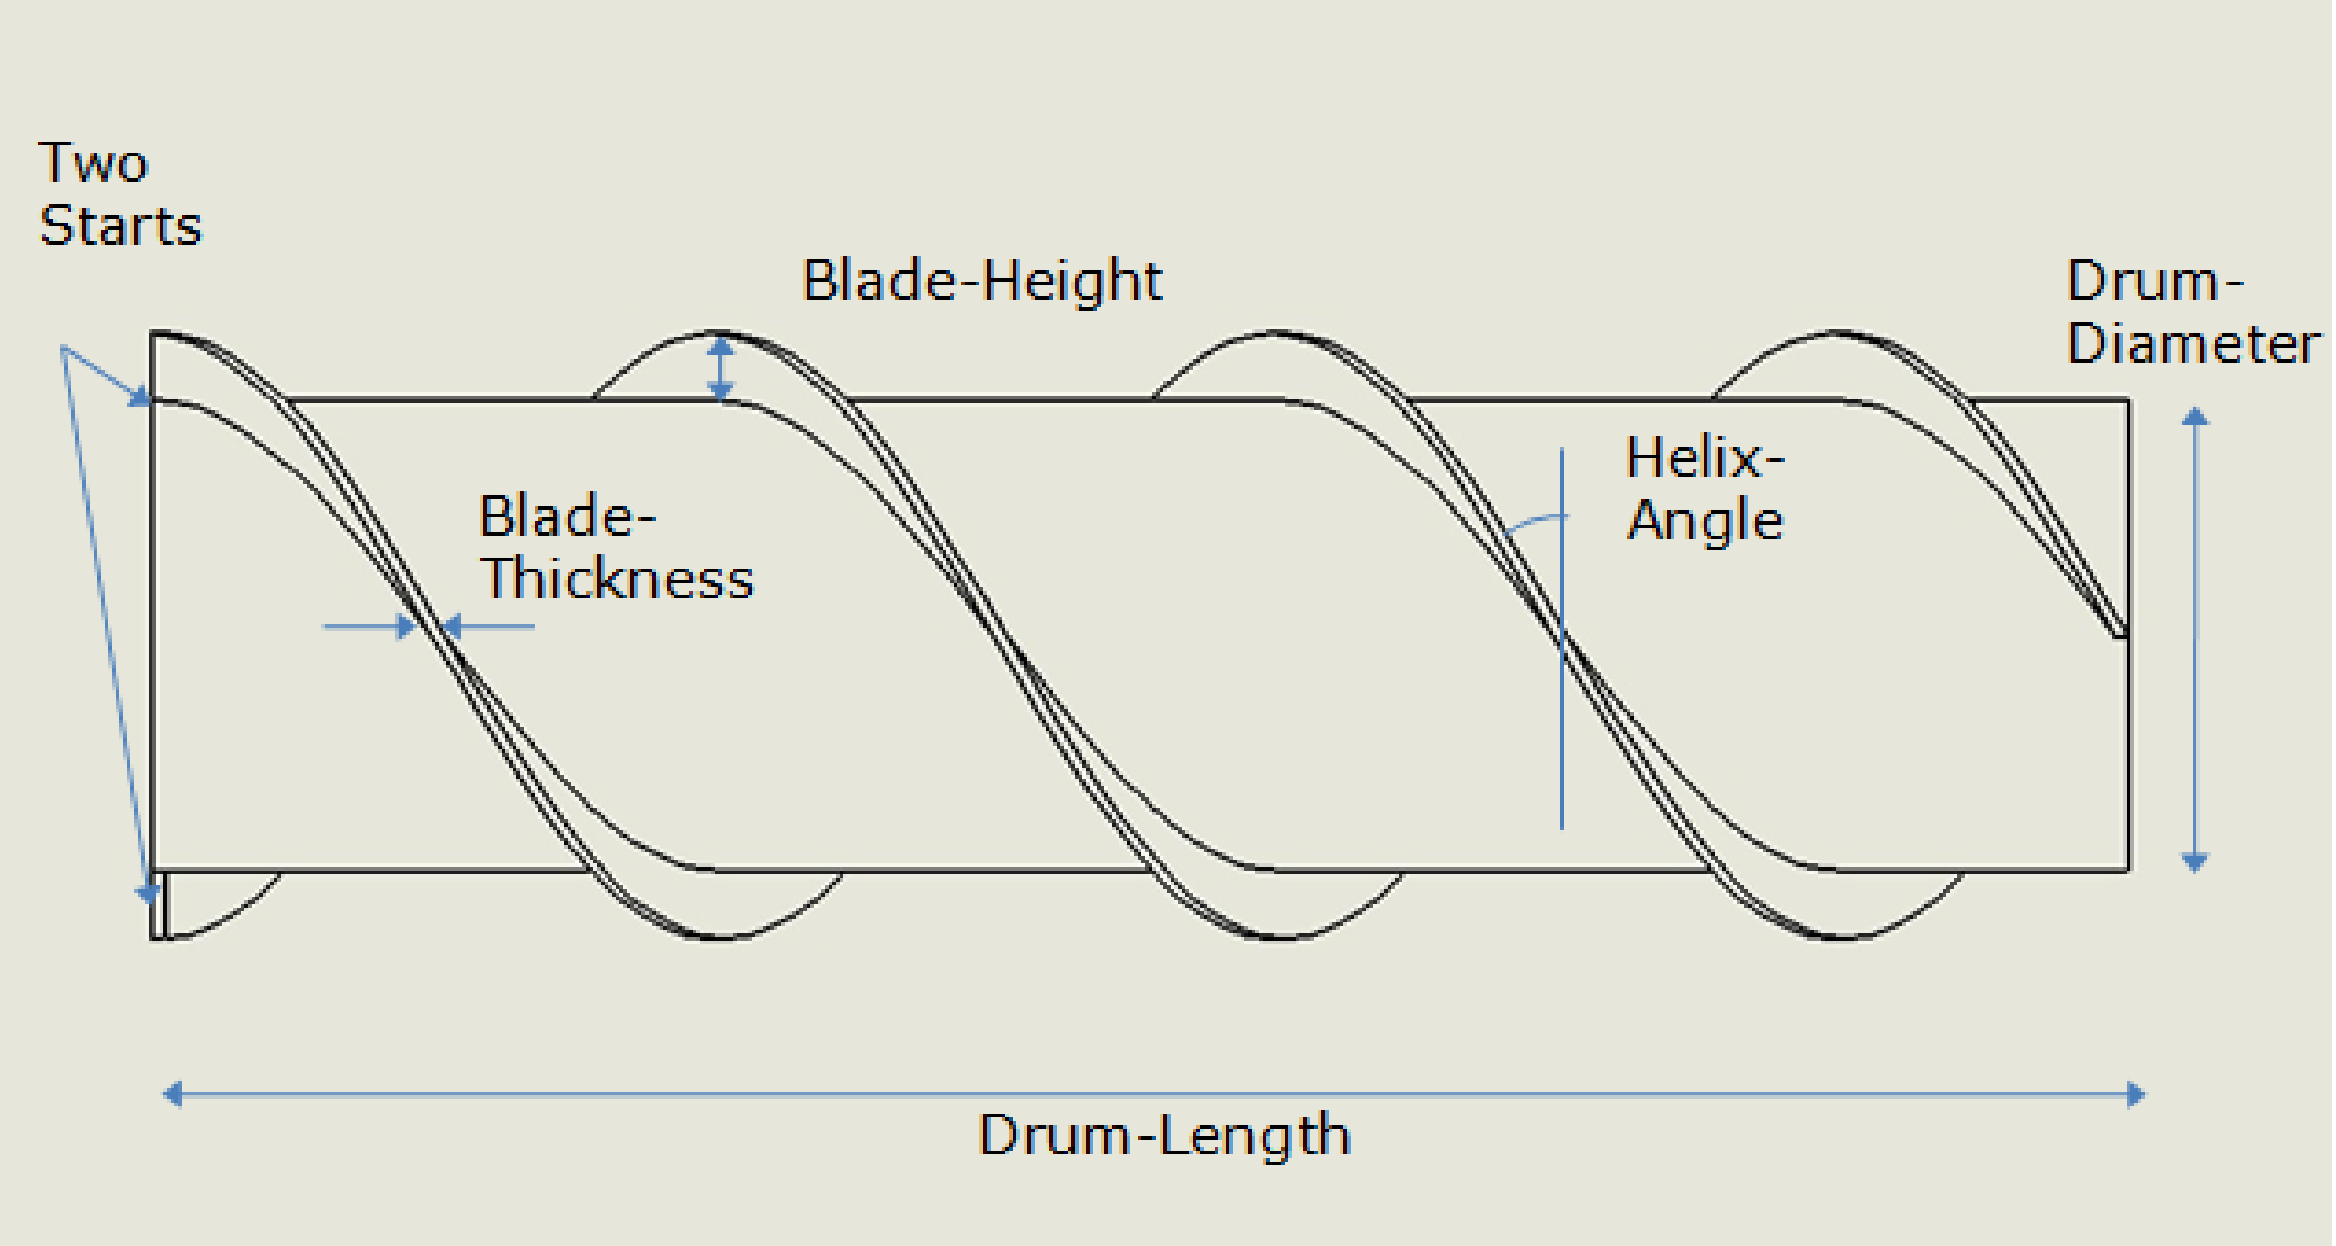
\includegraphics[trim=0 30 0 50,clip,width=0.9\columnwidth]{images/sd/screwdrive_parameters_freeberg.png}
	%\vspace{-10pt}
	\caption{Screw Design Parameters \cite{Freeberg2010}}
	\label{fig:screwdrive_parameters}
\end{figure}

%\begin{figure}[htb]
	%\begin{subfigure}[t]{0.5\textwidth}
		%\centering
		%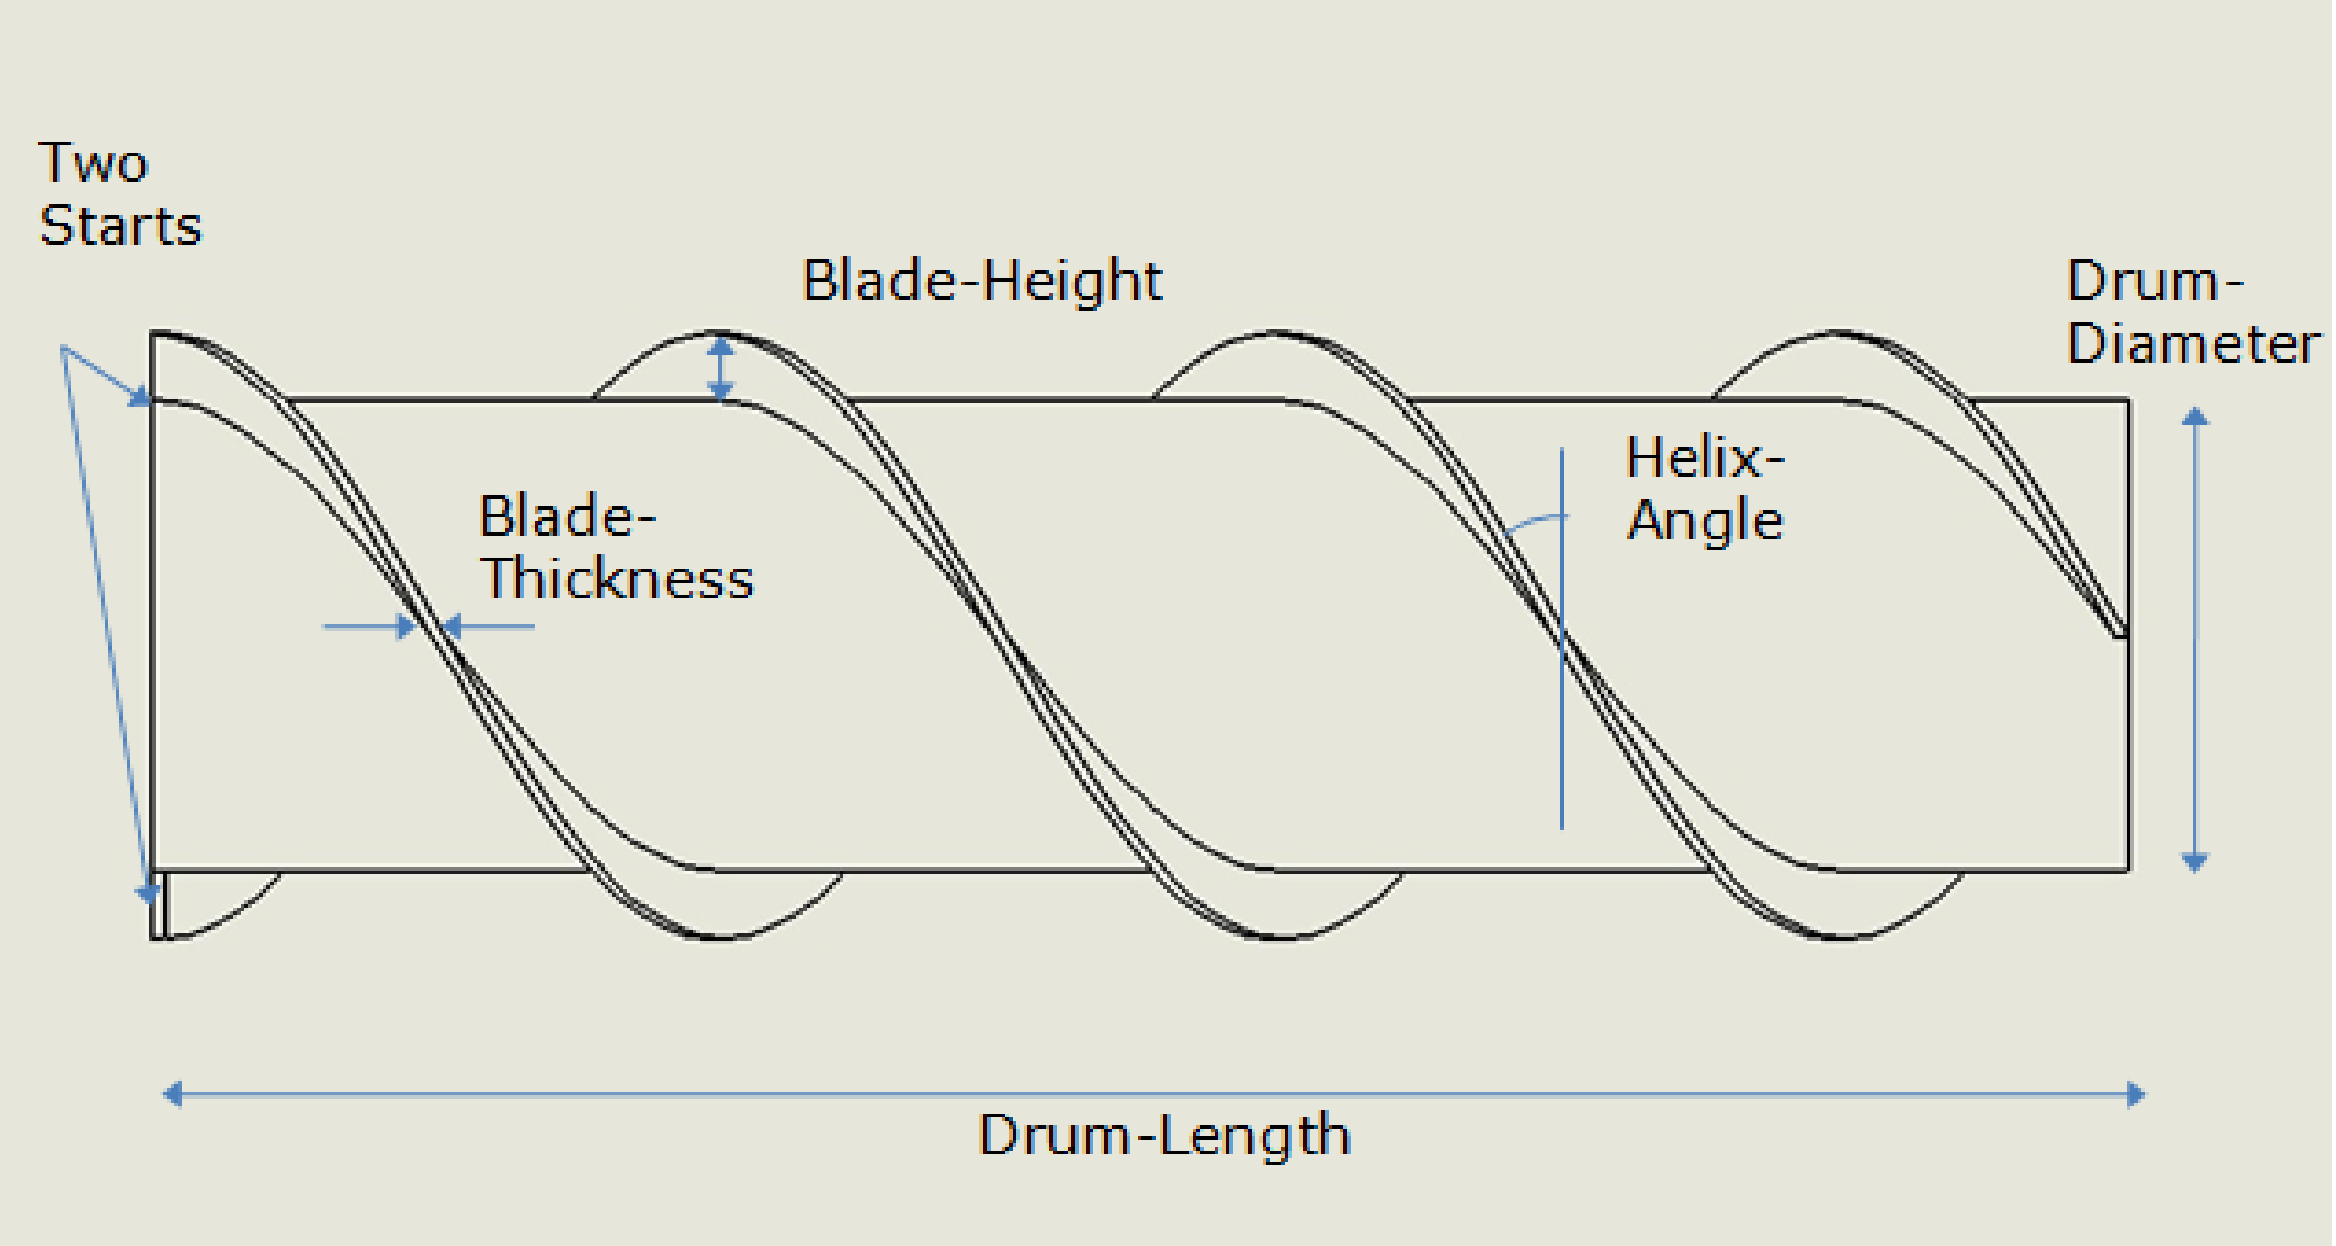
\includegraphics[width=1\columnwidth]{images/sd/screwdrive_parameters_freeberg.png}
		%\vspace{-10pt}
		%\caption{Screw Design Parameters \cite{Freeberg2010}}
		%%\vspace{-20pt}
		%\label{fig:screwdrive_parameters}
	%\end{subfigure}
	%\begin{subfigure}[t]{0.5\textwidth}
		%\centering
		%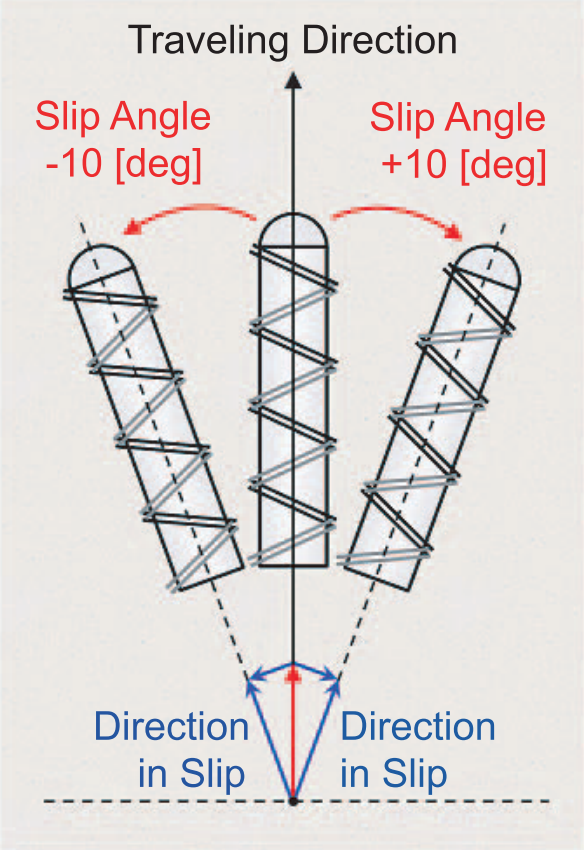
\includegraphics[width=0.5\columnwidth]{images/sd/screwdrive_slip_angle_nagaoka.PNG}
		%\caption{Slip angle \cite{Nagaoka2011}}
		%\label{fig:screwdrive_slip_angle} 
	%\end{subfigure}
	%\caption{Screwdrive characteristics}
	%\label{fig:screwdrive_characteristics}
%\end{figure}



%%screwdrive on aquapod
%\begin{figure}
	%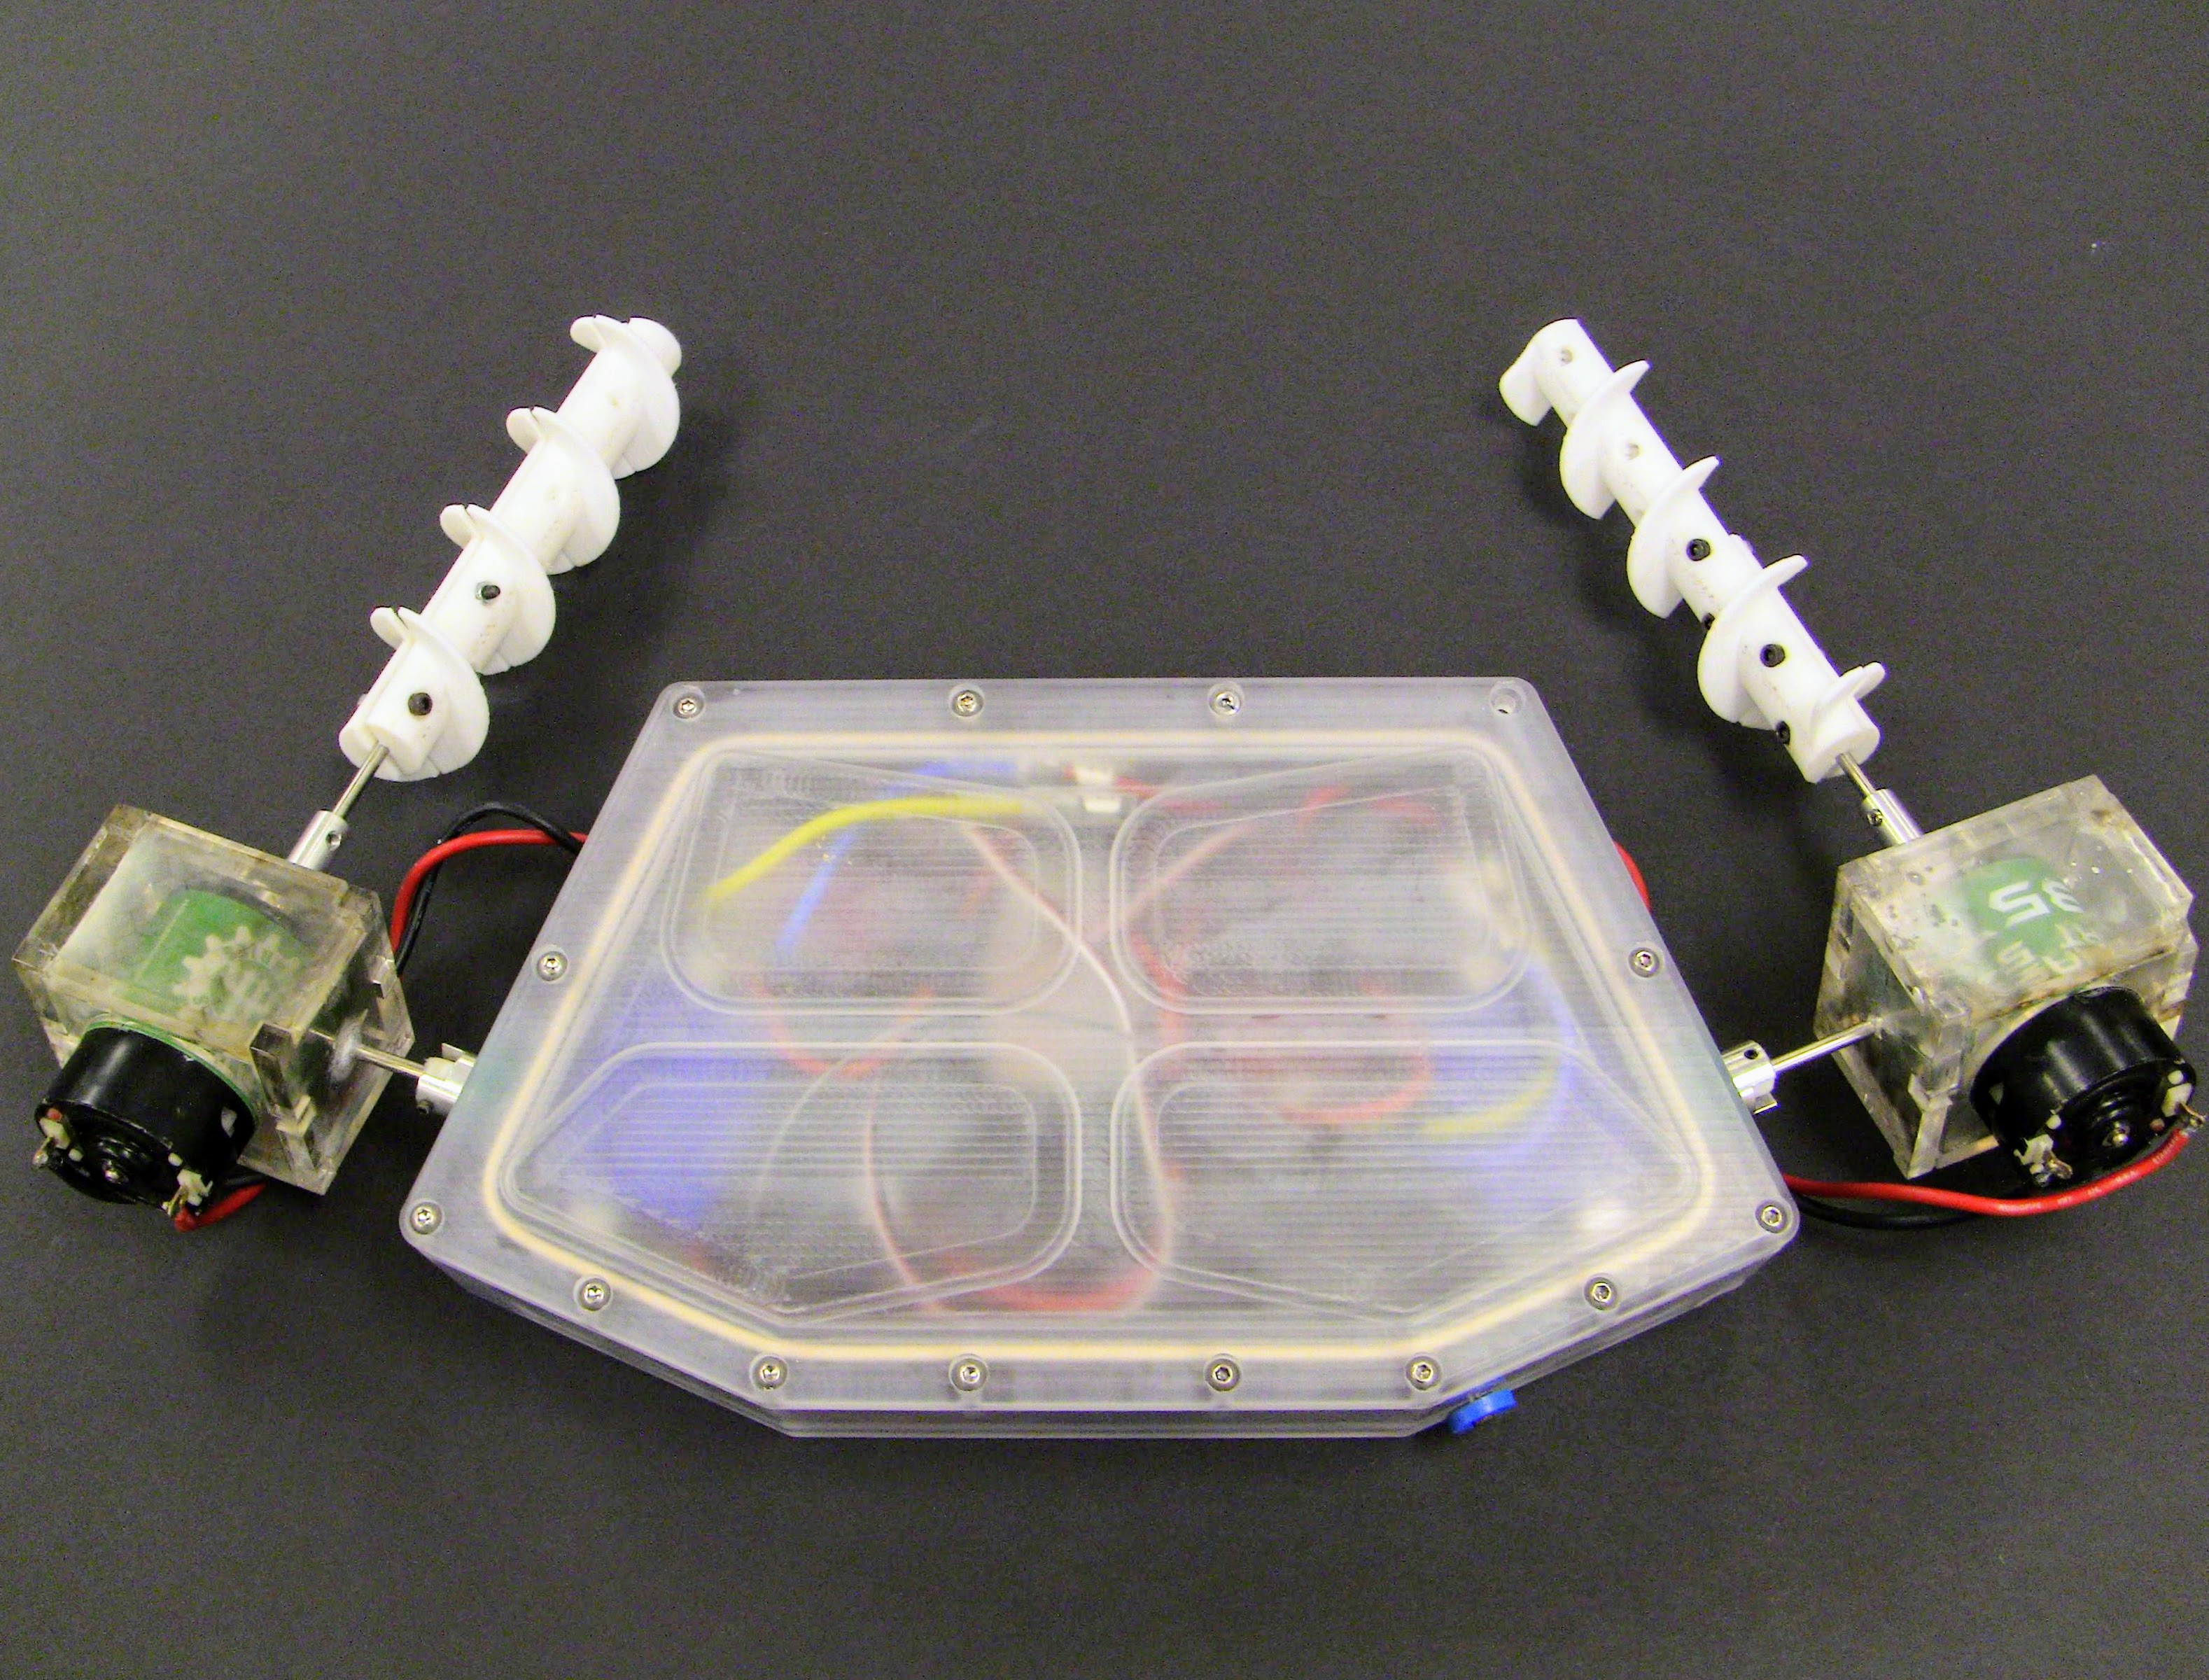
\includegraphics[width=\linewidth]{images/aquapod_v2_screwdrive.JPG}
	%\caption{The dual screwdrive arms on the Aquapod v1}
	%\label{fig:screwdrive_aquapod}
%\end{figure}

A screwdrive system is one that uses the rotation of one or more screws to generate motion. The majority of research in this area has focused on parallel dual-screw systems which consist of two contra-rotating screws are placed on either side of the vehicle body as a substitute for wheels or tank-treads. The Riverine Utility Craft and Dr. Cole's prototype, as seen on figure \ref{fig:screwdrive_prototypes}, are examples of dual-screw systems. 

%Figure~\ref{fig:screwdrive_aquapod} shows a dual-screw configuration in which the screws form an angle with respect to one another, this is called the \textbf{\emph{inter-screw angle}}. The inter-screw angle is important because it affects the resulting force balance between the screws, thereby affecting motion. 

The screw itself is comprised of two main parts: a barrel body and a blade that winds itself in a helical shape around the barrel body, as shown in Figure \ref{fig:screwdrive_parameters}. The barrel serves for mechanical support, and in some cases buoyancy, while the blade is the element that provides longitudinal locomotion. As the screw rotates, the blade travels longitudinally interacting with the medium against the blade. In the case of water, the displacement of the fluid provides thrust. In the case of a penetrable terrain, it is the combination of displacent and burrowing that provides the motion. In the case where there is no penetration of the medium by the blade, there would be no longitudinal component and rotation of the screw would be no different than rotation of a roller or wheel. 


The angle, \emph{\( \alpha \)}, that the blade makes with respect to the longitudinal axis of the screw is called the \emph{helix angle} or \emph{pitch angle}. The \emph{pitch angle} is one of the most influential parameters of a screw, as it determines the relationship between the rotational velocity and forward advance speed of the screw. The greater the \emph{helix angle}, the greater the rate of advancement. 

%TODO: COULD add image of screw with different pitches

%The screw blade is wound in a helix around the barrel body, as the screw rotates, the medium against the screw blade is pushed along the axis of the screw resulting in a longitudinal motion. In the case where there is no penetration, there would be no longitudinal component and rotation of the screw would be no different than rotation of a roller or wheel. 

The height, \emph{h}, of the blade is also an important parameter, as is the ratio of the blade height to the barrel diameter, this is referred to as \emph{blade-height-to-drum-diameter-ratio}. These parameters affect the amount of material the blade interacts with, which then influences thrust generated, torque requirements, drawbar-pull, among others. In a similar way, the number of starts the blade has, \emph{N}, is also important in controlling the amount of screw blade surface area in contact with the medium. Another geometric parameter of importance is the \emph{screw length}, this has also been expressed in terms of the \emph{length-to-drum-diameter-ratio} in studies. 

%The design of the screw itself is simple and enclosed, leading to robustness to mechanical failure and clogging when compared with other methods of locomotion\cite{Nagaoka2009b}. Screwdrives can function even when fully buried, this is advantageous in a number of situations such as snow, loose sand, mud, etc. 

The majority of the research into screw drive design and its parameters was conducted by Dr. Cole \cite{Cole1961} and Chrysler Defense Corporation \cite{Dugoff1967, Knight1965, Fales1972, Gorton1965} and utilized the parallel dual-screw configuration. On these screws, the helices were wound about the barrel in opposite handedness. Dr. Cole built scaled-down prototype seen in Figure ~\ref{fig:screwdrive_cole_model}, while Chrysler built 1/8 and 1/5 scale prototypes, to carry out parameter optimization and trials, before building the full scale Marsh Screw Amphibian (MSA) and the later Riverine Utility Craft (RUC), \ref{fig:screwdrive_ruc}.

%TODO: add Cole and Chrysler prototype images 
\begin{figure}[tb]
	\begin{subfigure}[t]{0.45\textwidth}
		\centering
		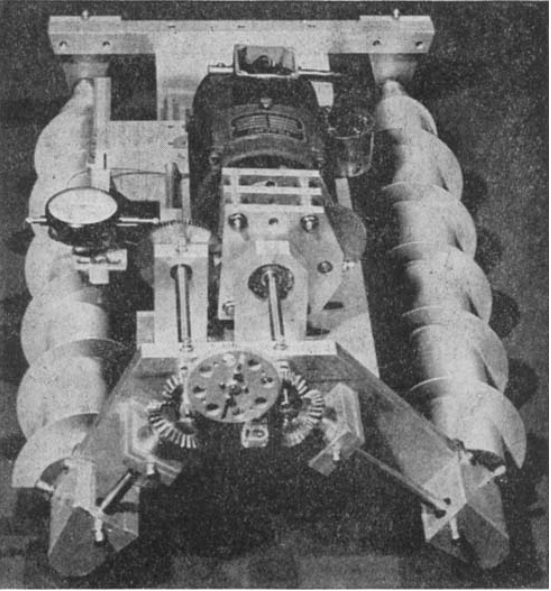
\includegraphics[width=1\columnwidth]{images/sd/screwdrive_cole_model.PNG}
		%\vspace{-10pt}
		\caption{Dr. Cole's prototype model \cite{Freeberg2010}}
		%\vspace{-20pt}
		\label{fig:screwdrive_cole_model}
	\end{subfigure}
	\begin{subfigure}[t]{0.55\textwidth}
		\centering
		%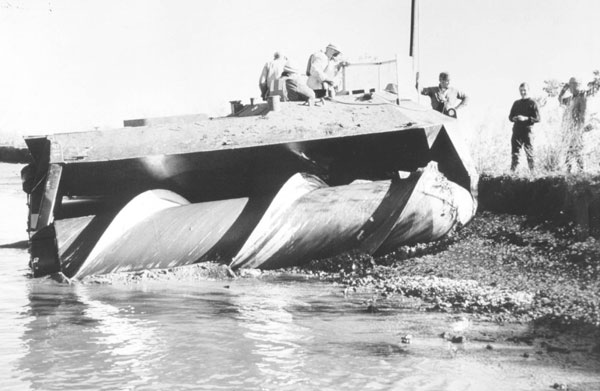
\includegraphics[width=1\columnwidth]{images/sd/screwdrive_ruc.PNG}
		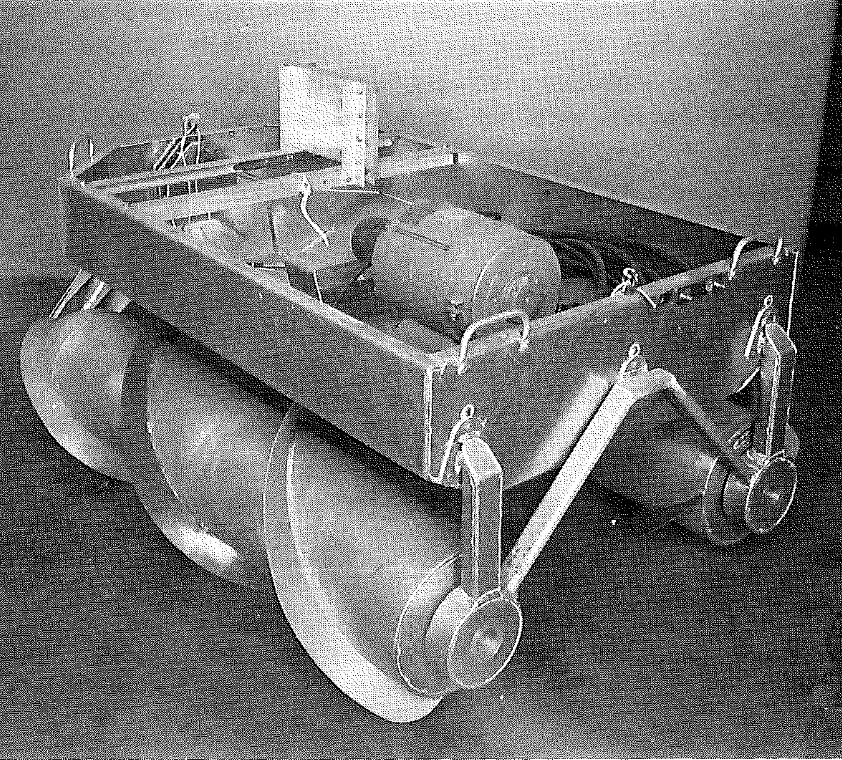
\includegraphics[trim=0 10 0 10,clip,width=1\columnwidth]{images/sd/screwdrive_ruc_fales.PNG}
		\caption{Riverine Utility Craft \cite{Fales1972}}
		\label{fig:screwdrive_ruc} 
	\end{subfigure}
	\caption{Screwdrive prototypes}
	\label{fig:screwdrive_prototypes}
\end{figure}

% other prototypes: http://www.oobject.com/category/9-screw-drivers/ 


Prototypes of various scales were built to evaluate and determine the optimal screw design parameters for water, ground, and  everything in between such as mud, snow, sand, and other terrains. The Marsh Screw Amphibian was tested in the Detroit River for more than 100 hours. 124 trafficability tests were performed in Louisiana by the US Army Engineer Waterways Experiment Station while a secondary MSA was built and tested for snow conditions in Houghton, Michigan \cite{Gorton1965}. 

Dr. Cole studied both screwdrive locomotion both aground and afloat. On ground, Cole \cite{Cole1961} found that vehicle performance gap, a measure of efficiency parameterized by screw slippage and power consumption, was less in the \emph{pitch-angle} range of 30 to 40 degrees than 20 to 30 degrees.  Drawbar-pull was almost maximum at 30 degrees, with little improvement with increasing helix angle. Therefore, from Cole et al. \cite{Cole1961} and Chrysler \cite{Dugoff1967, Fales1972} a value of 30 degrees or slightly greater was optimal. The Riverine Utility Craft \cite{Fales1972}, which was a continuation of the Marsh Screw Amphibian \cite{Dugoff1967}, utilized a pitch angle of 32 degrees.

With respect to \emph{blade-height-to-drum-diameter-ratio}, Cole used 0.375 as the ratio in his experiments finding it a sufficient tradeoff between propulsive surface area and structural integrity of the blades. Dugoff et al. \cite{Dugoff1967} utilized ratios of 0.125, 0.167, and 0.208 and found that increasing the height also increased the amount of media moved, however, its effect on drawbar-pull was minimal in sand. On mud, an increase in height resulted in decreasing performance due to greater likelihood of bogging down. Eventually 0.125 was chosen as an ideal ratio.

%Another important parameter is the \emph{number of starts}, while Chrysler does not make available data on the number of starts, both the MSA and the RUC \cite{Knight1965} used two screw starts, with Dr. Cole making the case that two starts may grant better dynamic balancing. 

Unlike the monotonic effects of the \emph{helix angle} and \emph{screw blade height} on the drawbar-pull capacity, the \textbf{\emph{length-to-drum-diameter-ratio}} was found to follow a concave curve. These studies were carried out for mud and sand and, coincidentally, the optimal value for both terrains occurred at around 6. In water, Dr. Cole found that longer screws led to more rotations and consequently larger driving torques and thrust.  

%Although important in terms of design and manufacture, \emph{blade thickness} was not studied explicitly. It was noted that during operation, the Riverine Utility Craft screws began to develop cracks along the blade. The cause of the cracks was thought to be from forces on the screw blade, given that the screws had passed preliminary shock tests. The solution was to this problem was to add structural reinforcement to the back of the screw blade. 

Not a parameter of the screw itself, the \emph{center-of-gravity} affects the pitch of the vehicle, leading to bulldozing or plowing if located too far forward and suboptimal performance if placed too far towards the rear \cite{Dugoff1967, Nagaoka2011}. 

%The \emph{slip angle} is another parameter that is not of the screw but affects the function of the vehicle. Experiments on a custom rig showed that drawbar pull increased significantly when the slip angle, which is the angle of the screw relative to motion of the vehicle, was deviated from parallel for a variety of speeds. Furthermore, the drawbar pull displayed increased for positive angles, but decreased with negative slip angle. This would suggest that the more perpendicular the screw blade is relative to vehicle motion, the larger the drawbar pull. This would also correlate other experiments from Nagaoka \cite{Cole1961} that measured drawbar-pull against \emph{helix angle}. If this is the case, one could alter the screws' \textbf{\emph{helix angle}} to compensate for screws that are oriented at an arbitrary \textbf{\emph{slip angle}} with respect to the vehicle's body, such as the Aquapod as seen in Figure ~\ref{fig:screwdrive_aquapod}, to obtain optimal performance.

Clearly, the parameters of the screws affect a screwdrive system's performance on a given terrain, while Dugoff et al. \cite{Dugoff1967} utilized parameters that balanced the performance on water and on land, there exist parameter configurations that maximize screw performance in other domains. Furthermore, while Cole \cite{Cole1961} and Dugoff \cite{Dugoff1967} both studied screw parameters, blade penetration of the terrain was greatly facilitated by the relatively heavy weight of the tank-sized vehicles. %Additionally, while drawbar pull, or towing capacity, was an important outcome metric for the aforementioned applications, at the smaller and lighter scale of environmental robotics, parameters to increase mobility would be more relevant. 

%In the next section the maneuverability of screwdriven vehicles is explored. 

%The parameters mentioned affect the ability and the way that a screwdrive propelled vehicle moves throughout an environment. In the next section the maneuverability of screwdriven vehicles is explored. 

%Nagaoka \cite{Nagaoka2011} and Cole \cite{Cole1961} showed that forward speed was proportional to rotational speed, therefore indicating constant slip conditions. % #parameters %TODO: check on Cole/Dugoff reference for forward-speed to rotational velocity relation independence on other factors. 

	%\emph{Inter-screw angle:} the inter-screw angle is the angle between two or more screws. This angle playes a pivotal role as it affects the interplay of forces and resulting motion of a vehicle. In systems with two independently actuated screws, the inter-screw angle affects the resulting motions from the net forces of the competing or cooperating screws. The redirection and interplay of the forces from the dual-screw set-up can be seen in Figure~\ref{fig:screw_FBD_alpha_0} and Figure~\ref{fig:screw_FBD_alpha_45} where the inter-screw angle is set to 0 and 45 degrees, respectively. Figure~\ref{fig:screw_FBD_alpha_0} shows the direction of the force when the blade is engaged. This mode is optimal for a screwdrive system because the direction of the force together with the independence of the actuators can be used to move the vehicle forward, backward, laterally, and to allow rotations in place, in effect, omnidirectional locomotion. 

%\begin{figure}[ht]
%	\centering
%	\includegraphics[scale=0.25]{images/screw_propulsion_FBD_alpha_0.pdf}
%    \caption{Inter-screw angle of 0 degrees (parallel)}
%	\label{fig:screw_FBD_alpha_0} 
%\end{figure}
%\begin{figure}[th]
%	\centering
%	\includegraphics[scale=0.25]{images/screw_propulsion_FBD_alpha_45.pdf}
%    \caption{Inter-screw angle of 45 degrees}
%	\label{fig:screw_FBD_alpha_45} 
%\end{figure}

%------------------------------------------------------------------------------------------------
\subsubsection{Maneuverability}
\label{sec:screwdrive_maneuverability}
%------------------------------------------------------------------------------------------------

\begin{figure}[t]
	\centering
	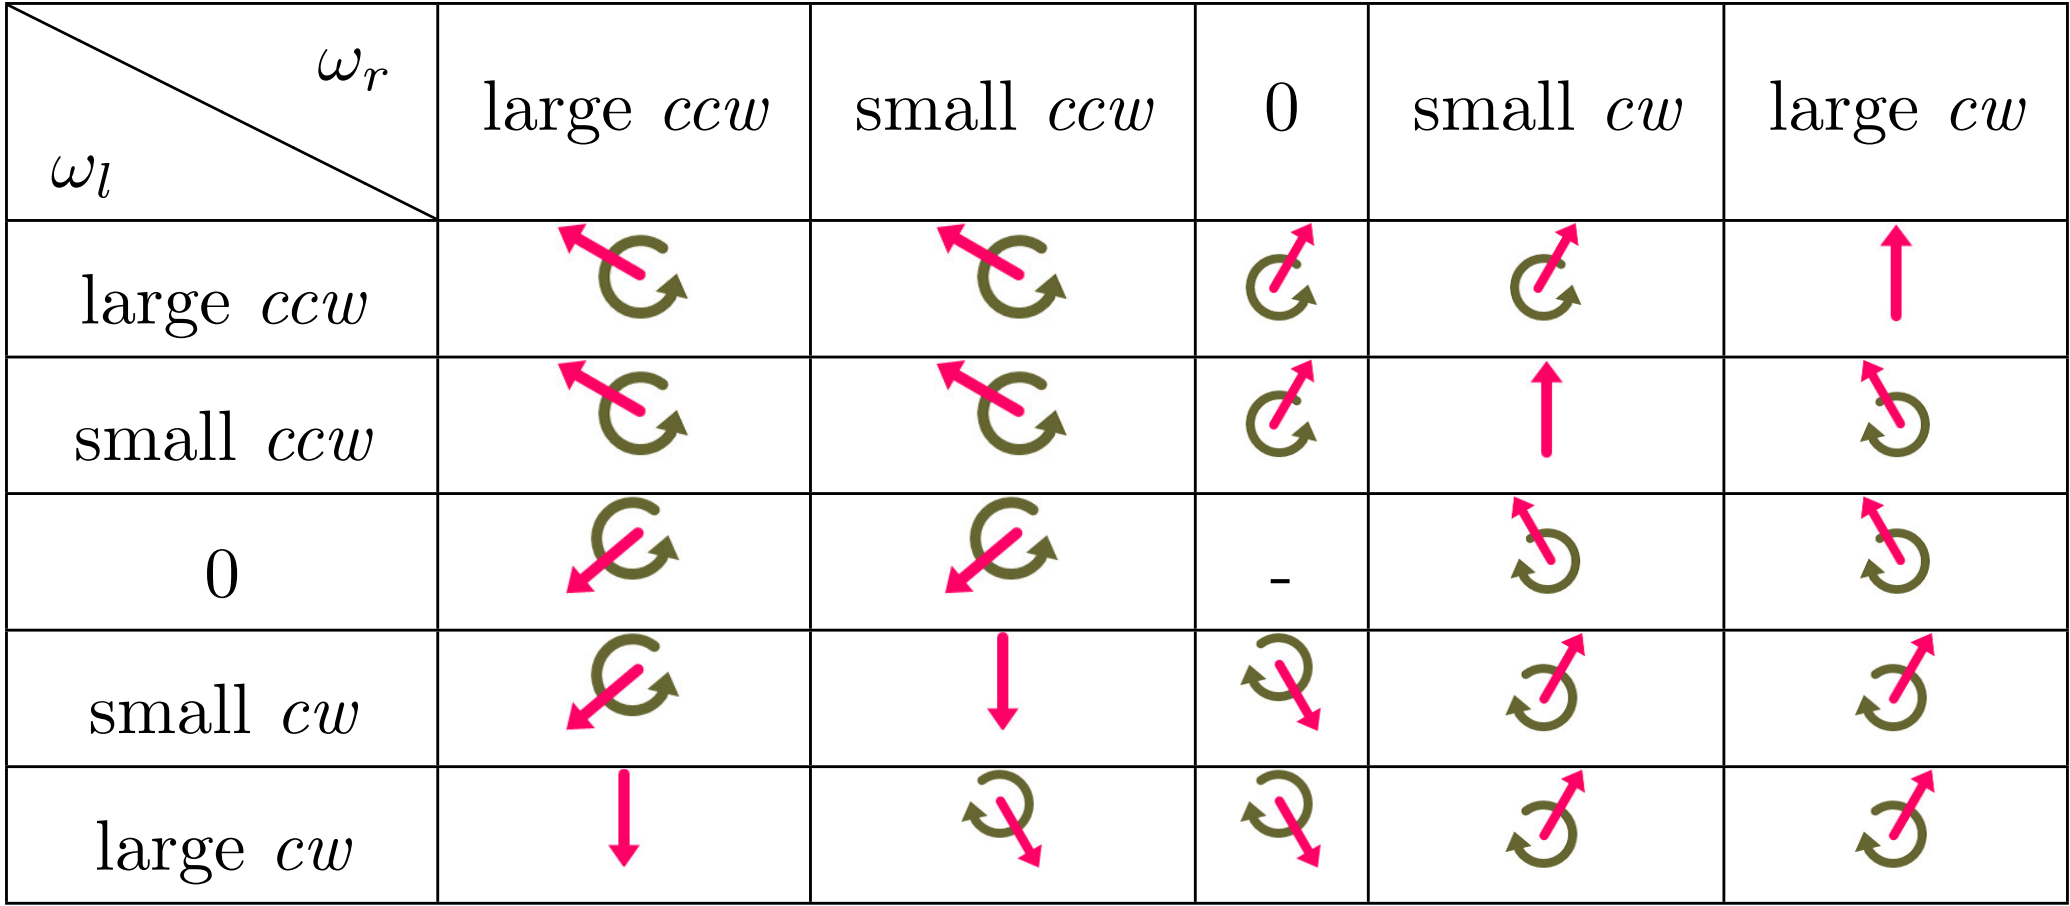
\includegraphics[width=1\columnwidth]{images/sd/screwdrive_maneuverability_nagaoka.png}
	\vspace{-10pt}
	\caption{Screwdrive Maneuverability \cite{Nagaoka2009a}}	
	%\vspace{-20pt}
	\label{fig:screwdrive_maneuverability}
\end{figure}


%\begin{figure}[ht]
	%\begin{subfigure}[t]{0.5\textwidth}
		%\centering
		%%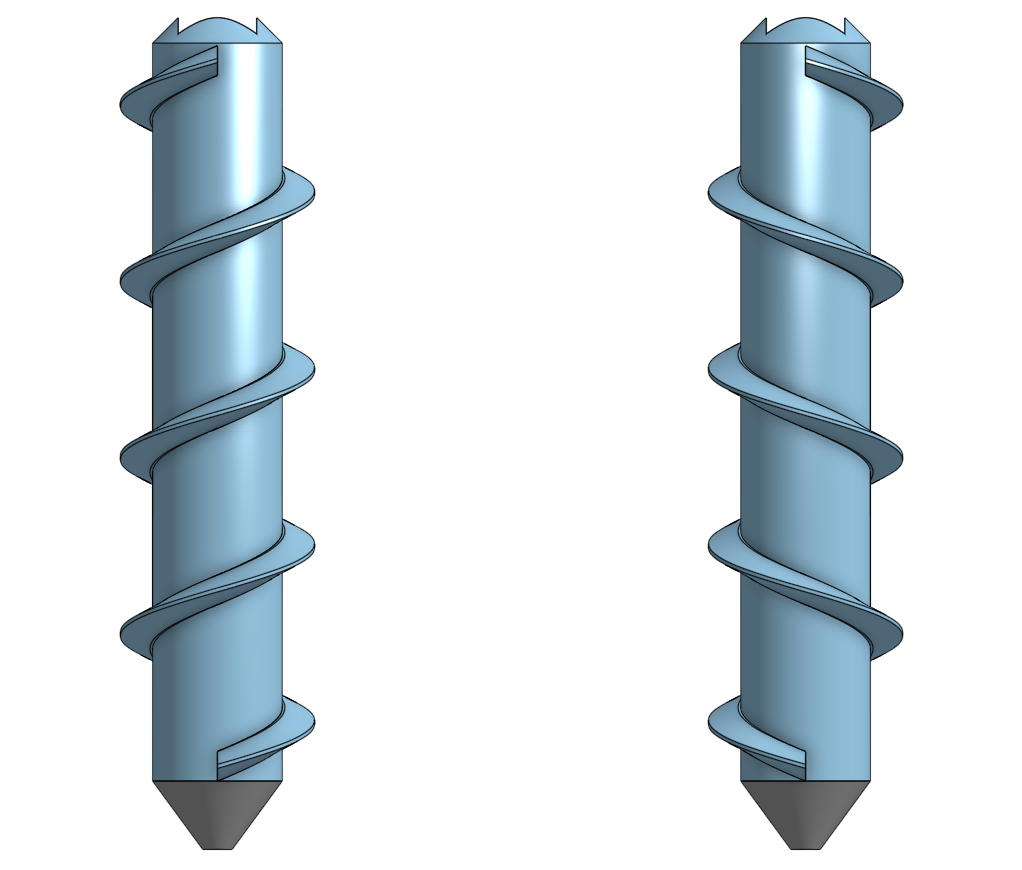
\includegraphics[width=1\columnwidth]{images/sd/screws_renders_dual_top.png}
		%\includegraphics[width=1\columnwidth]{images/sd/screw_propulsion_FBD_alpha_0.pdf}
		%\caption{Inter-screw angle of 0 degrees (parallel)}
		%\label{fig:screw_FBD_alpha_0} 
	%\end{subfigure}
	%\begin{subfigure}[t]{0.5\textwidth}
		%\centering
		%%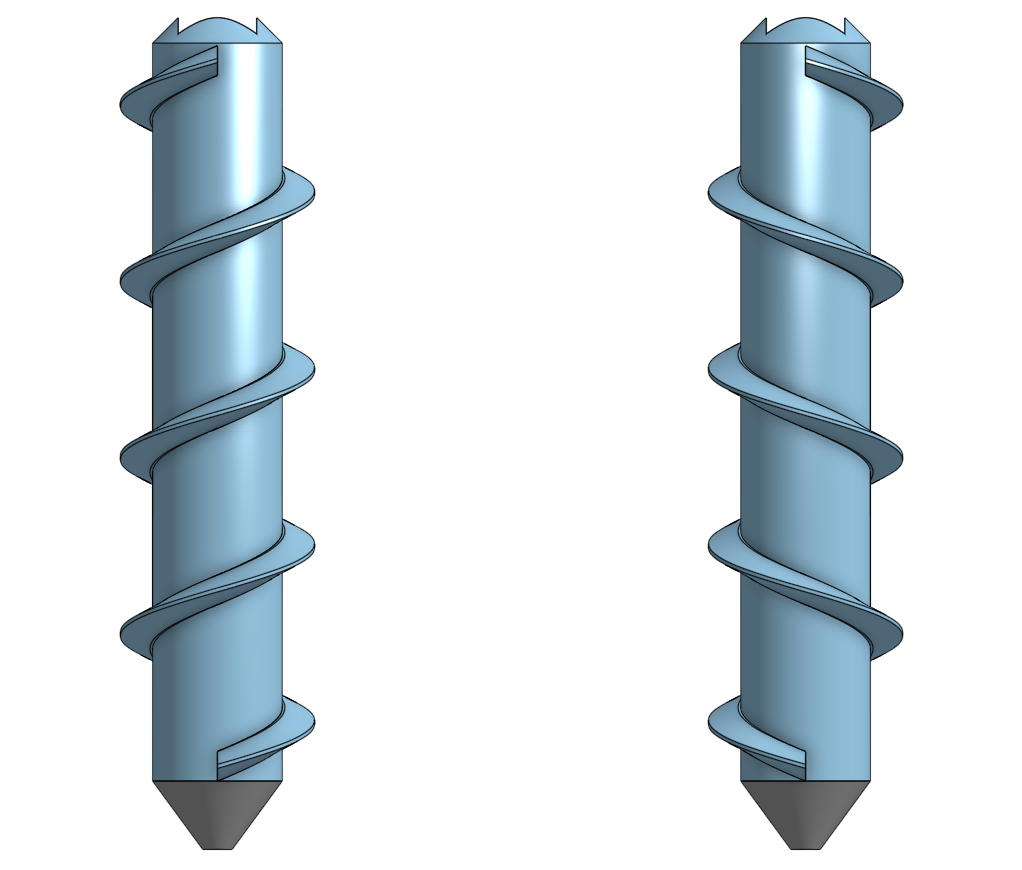
\includegraphics[width=1\columnwidth]{images/sd/screws_renders_dual_top.png}
		%\includegraphics[width=1\columnwidth]{images/sd/FBD_two_screw_45_rigid_rotation.pdf}
		%\caption{Inter-screw angle of 45 degrees}
		%\label{fig:screw_FBD_alpha_45} 
	%\end{subfigure}
	%\caption{Screwdrive FBD Models}
	%\label{fig:screwdrive_renders}
%\end{figure}


%\begin{figure}[ht]
	%\begin{subfigure}[t]{0.5\textwidth}
		%\centering
		%\includegraphics[width=1\columnwidth]{images/sd/screw_propulsion_FBD_alpha_0.pdf}
		%\caption{Inter-screw angle of 0 degrees (parallel)}
		%\label{fig:screw_FBD_alpha_0} 
	%\end{subfigure}
	%\begin{subfigure}[t]{0.5\textwidth}
		%\centering
		%\includegraphics[width=1\columnwidth]{images/sd/screw_propulsion_FBD_alpha_45.pdf}
		%\caption{Inter-screw angle of 45 degrees}
		%\label{fig:screw_FBD_alpha_45} 
	%\end{subfigure}
	%\caption{TEST}
	%\label{fig:TESTS}
%\end{figure}

Research into screwdrive locomotion is centered, in large part, around its function in compliant media, such as soft terrains or fluids \cite{Dugoff1967, Cole1961, Nagaoka2011, Freeberg2010, Fales1972}, as this is where screwdrive systems excel. The degree of penetrability of the screw blade affects performance of the screws and consequentially a screwdriven vehicle. 

On rigid terrains where the blade cannot penetrate, the screwdrive behaves very differently both from a modeling and maneuverability perspective. Therefore, the screwdrive is dependent not only on the aforementioned geometric and functional parameters covered in section \ref{sec:screwdrive_parameters} but also on the properties of the medium it's in as well as the bearing load on the screws. 

% Force definition:
Screws provide a combination of tractive and rolling forces. \textbf{\emph{Rolling }} forces are those that result from oppositional frictional forces upon the body of the screw as it rotates, like a wheel, about its axis. These forces can be visualized as the forces that would be present were the screw blade not present, i.e. as if the screw was instead a roller. The addition of the screw blade adds \textbf{\emph{tractive}} forces. As the screw rotates, the blade displaces and moves along the medium adjacent to the blade surface creating longitudinal and lateral components of tractive force. The balance between the lateral and longitudinal components of the tractive force is highly dependent on the \emph{pitch angle}.

% TODO: add figure with force vectors 
Description of rolling and tractive forces depend on complex terramechanics models \cite{Nagaoka2010a, Cole1961}, fortunately, a more simple approach to these forces can be taken in order to determine the maneuverability of a screwdriven vehicle. Freeberg \cite{Freeberg2010} and Nagaoka et al. \cite{Nagaoka2009b} treat the rolling force similarly, while differing on their treatment of the tractive force. Nagaoka assumes the tractive force direction as perpendicular to the screw blade face, hence dependent on the \textbf{\emph{pitch angle}} and decomposable into longitudinal and lateral components, whereas Freeberg keeps only the longitudinal component of the tractive force. The combination of these \textbf{\emph{tractive}} and \textbf{\emph{rolling}} forces determine the resulting motion of the vehicle. 

Maneuverability is controlled by the ability of the screw to penetrate the medium, the relative orientation of the screws with respect to one another, and the screws' placement with respect to the vehicle body. When the screw penetrates the terrain, it has been found that the tractive forces dominate the rolling forces, the opposite has been found on rigid terrains. One exception found by Nagaoka \cite{Nagaoka2009a} is the case where the screws are rotating at a very slow speed in a penetrable terrain, under these conditions, the tractive forces do not outright dominate the rolling forces and some unwanted sideways motion is observed. Another exception has been documented \cite{Cole1961} when transitioning from water to land, when the vehicle will lurch as the screw initially rolls on the ground. 
%In Figure~\ref{fig:screw_FBD_alpha_0} two contra-rotating screws are shown.

The motions of a dual-screwdrive system in a penetrable terrain are shown in Figure ~\ref{fig:screwdrive_maneuverability}. These are shown from Nagaoka et al. \cite{Nagaoka2009a}, however, Freeberg's \cite{Freeberg2010} research is also in accordance. These motions arise from the combination of one of three actions possible through each of the two motors: clockwise, counterclockwise, or no rotational velocity. 

Since the screws are oppositely handed, longitudinal locomotion is achieved through contra-rotation of the screws at the same speed. This results in forward or backwards motion depending on the combination of the handedness of the screws and direction of screw rotation. The next case, skid turning, is that when one of the screws rotates and the other does not. Skid-turning results in a desirable tight-radius turn, however, it is terrain dependent and there are some situations where skid turning may not be optimum. Under low friction and low cohesion aground conditions, such as loose sand, skid-turning can result in the screw burying itself. In higher friction or highly cohesive terrains, such as clay, skid turning may not be possible as this requires more force. Finally, when both screws turn in the same direction there are two motions possible dependent, once again, on terrain. In water, this leads to a rotation of the vehicle with no net traversal motion, this is known as point-turning. Aground, it leads to arc-turning of various radii, depending on the type of terrain. %Freeberg \cite{Freeberg2010}, found that clay, gravel, loose sand, and dirt produced wide arcs, whereas grass and marshlands procuded smaller-radius arc. The commonality being that these motions involved a rotation of the vehicle as well as a net displacement. 

%Nagaoka et al. \cite{Nagaoka2009a} also explored the case where both screws were actuated but at different directions and speeds, producing arc turning, which they refer to as steering. This steering is useful as it would permit adjustments to heading while the robot is in motion. 

\subsubsection{Variable Geometry Screws Origami}
\label{sec:screwdrive_variable_pitch}

\begin{figure}[htb]
    \begin{subfigure}{0.5\textwidth}
    \centering
    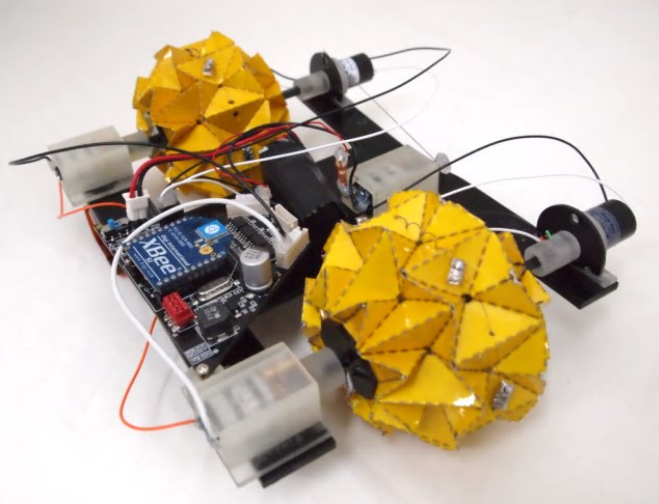
\includegraphics[width=.90\columnwidth]{images/origami_lee2013.png}
    \caption{Deformable wheel robot, \cite{Lee2013}.}
    %\vspace{-20pt}
    \label{fig:origami_lee}
    \end{subfigure}
    \begin{subfigure}{0.5\textwidth}
    \centering
    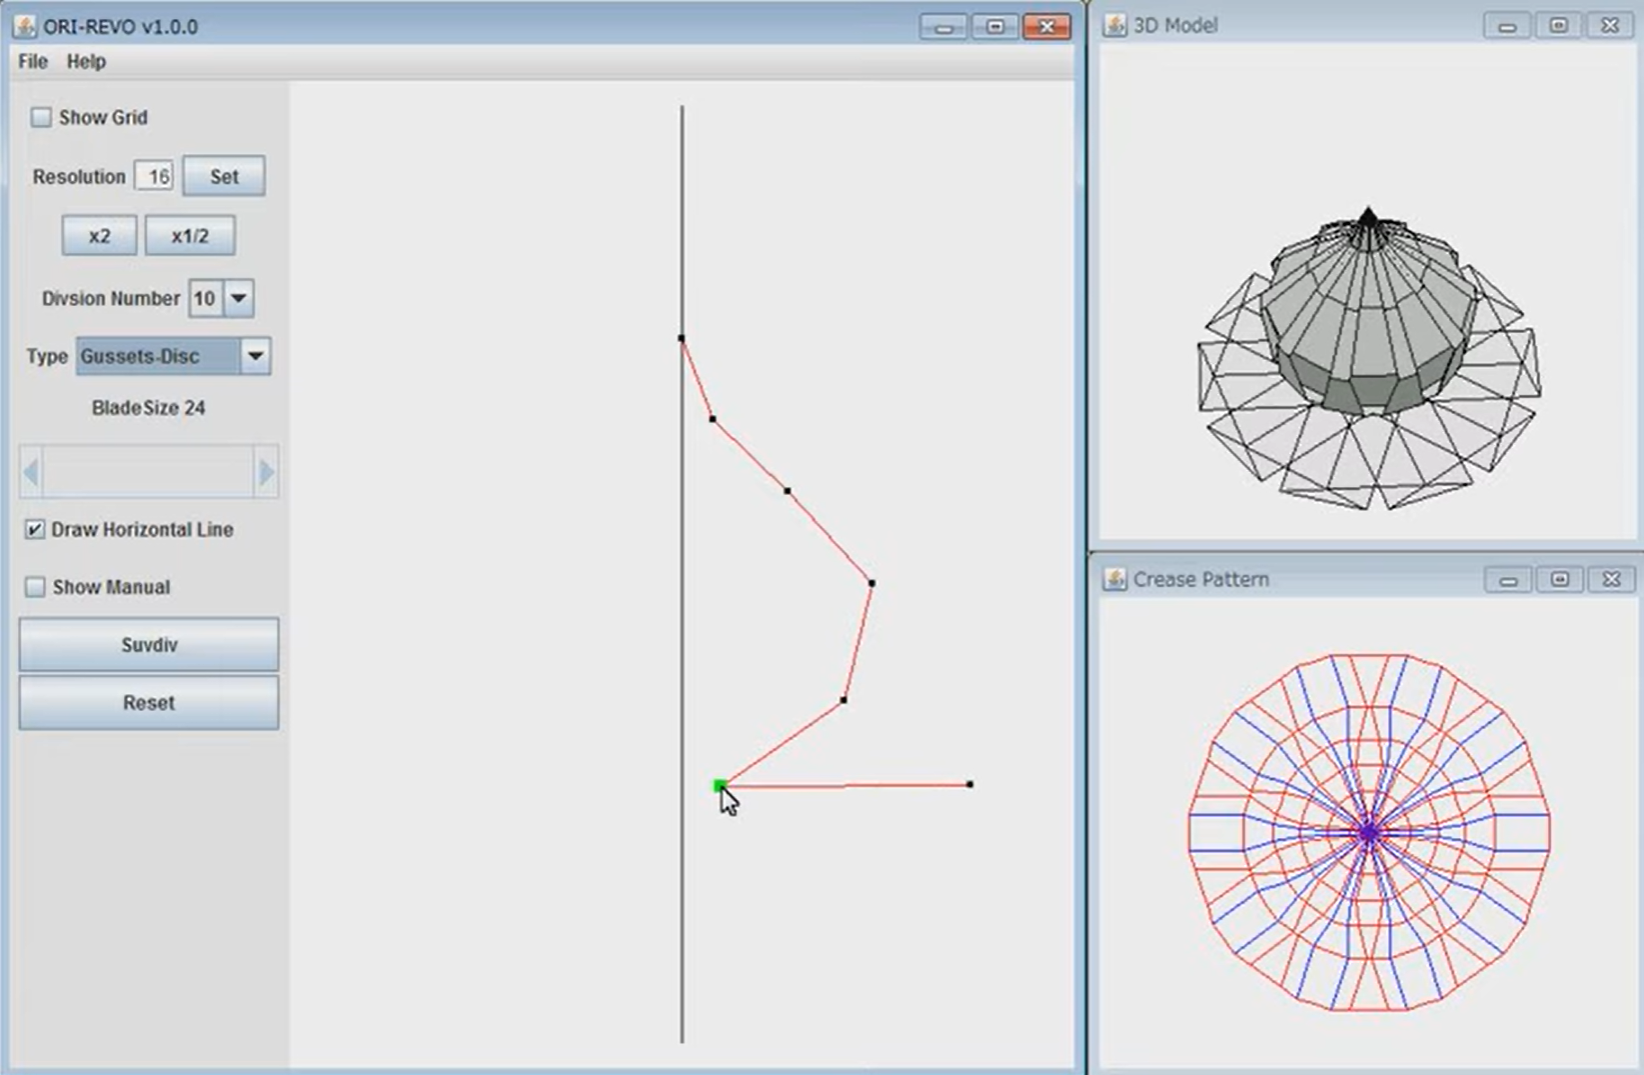
\includegraphics[width=1.10\columnwidth]{images/origami_orirevo.png}
    \caption{ORI-REVO software, \cite{Mitani2009}.}
    %\vspace{-20pt}
    \label{fig:origami_orirevo}
    \end{subfigure}
    \caption{Origami applications and software}
    \label{fig:origami_lee_orirevo}
\end{figure}

%\begin{figure}[!htb]
		%\centering
		%
\includegraphics[width=.90\columnwidth]{images/origami_tachi2010_complex_real.png}
		%\caption{Origami structures, \cite{Tachi2010}.}
		%\vspace{-20pt}
		%\label{fig:origami_tachi_complex_real}
%\end{figure}


%Motivation
Once optimal screw parameters for a given set of terrains are found and an onboard terrain classification system provides the type of terrain, a variable pitch screw would allow switching between different sets of geometries to best suit the terrain. 

Origami is an art form that is increasingly being looked to for its ability to create folding structures from a two dimensional pattern, from MEMS devices \cite{yan2016}, to robotic crawling actuators \cite{Rafsanjani2018}, to deformable wheels \cite{Lee2013}, and medical microrobots \cite{Miyashita2015} this technique allows creation of metamaterials that can be actuated with a single degree of freedom. In metamaterials, the resulting structure depends not only on the underlying construction material, but also the geometry, leading to structures that can exhibit wildly different properties, such as stiffness, compressive moduli, etc, than their base material. 

%Current fabrication methods for the screws utilize three dimensional printing. While useful for initial prototypes, utilizing a laser cutter would decrease fabrication time significantly as Silverberg et al. \cite{Silverberg2015} and Rafsanjani \cite{Rafsanjani2018} have found. Furthermore, this fabrication method could provide the means by which to design and fabricate a robust variable pitch screw with a high degree of robustness as compared to an articulated variable pitch device. 

%Furthermore, generating origami via traditional hand-folding methods, while simple, creates pre-creases in the material that are not necessary in the final structure but are nevertheless present and affect stiffness, adding additional degrees of freedom to the structure. 

%In \cite{Silverberg2014a} Silverberg utilized dash-and-gap perforations since it was found that continuous line patterns lead to lattices that are easy to tear and exhibit anisotropic bending properties. Dash-and-gap, on the other hand, allowed isotropic bending properties and equal folding stiffness for valley and mountain creases. 

%Another form of manufacture would be a two step process where the laser would make engravings of mountain or valley folds instead of cutting all the way through. This would lead to a stronger and sealed surface which is desirable ingress protection. 

Lee et al.\cite{Lee2013} create an active origami wheel using the waterbomb, or magic ball, origami pattern for the structure and a combination of passive elements, such as a spring, and smart wire actuators to achieve changes in its shape, Figure ~\ref{fig:origami_lee}. Silverberg et al. \cite{Silverberg2015} utilize the Miura-ori tesselated folding pattern to create structures comprised of individual cells that are bistable, that is they settle into decreased energy minima. This switchable behavior would be pertinent in actuator design as it would allow structures that have two stable passive states with energy needed only to switch states. 

%The magic ball pattern is comprised of individual unit structures, in this case triangles, that exhibit independent behavior but can be chained to produce a bulk structure composed of individual switchable units, as in Figure ~\ref{fig:origami_lee}. 

%Furthermore, they showed that many structures can arise from the same underlying patterns by localized push-through-defects. One could imagine a robot hull made of a Miura-ori tesselated surface where each unit cell is actuated via an individual actuator to change the outer structure of the robot in real-time. 

With this project, we propose development of a screw using origami principles to achieve an actuatable surface capable of transitioning between two distinct stable configurations and where the limits are set either mechanically or by exploiting origami bistability. 

% inverse design problem 
In order to do this a crease pattern needs to be generated to create the target design, this is known as the inverse design problem. Castle et al. \cite{Castle2014} programatically tackle the inverse problem of designing cuts and folds in a 2D surface to obtain a given 3D object. 

Mitani et al. \cite{Mitani2009} created the ORI-REVO software which allows creation of revolution surfaces by specifying a profile pattern, see Figure ~\ref{fig:origami_orirevo}. This tool also allows the specification of division number, resolution, as well as manual manipulation in real time. The resultant 3D form is shown in the top right and the crease pattern in the bottom right. %rotational symmetry

Morever actuation forces need to be computed in order to specify the actuator. Fuchi et al. \cite{Fuchi2013} have developed OMTO (an origami modeling toolbox for matlab) which uses FEM to set boundary conditions, fixed points, and forced point to calculate fold lines that optimize greatest displacement in specified directions at the output nodes. In 2018, Gillman \cite{Gillman2018} continued this work adding nonlinear optimization yet removing the graphical user interface. 

\subsubsection{Proposed Research}
%Screwdrive locomotion is feasible and desireable as a simple, robust, and inexpensive form of amphibious locomotion. As with any novel method of locomotion, more research is needed to appropriately describe its nuanced aspects. In particular, 

It has been shown that while screwdrive locomotion works well aground and afloat, its maneuverability, motion model, and design parameters differ for both limit scenarios. Moreover, within aground performance, parameter and locomotion strategies can change not only based on the type of terrain (snow, sand, dirt) but also on time-dependent conditions, such as friction and cohesion, which are dependent on the level of moisture in the ground.

Given the variable nature of the terrain and types of terrain a screwdrive vehicle is capable of navigating, developing a dynamic model that learns its parameters in real-time would be advantageous. This online model would also allow detection of transition between different terrains, in particular aground and afloat conditions, and react accordingly. This model would build on the efforts of \cite{Rogers-Marcovitz2014} et. al, who used an Extended Kalman Filter to identify changing parameters of the models based off predicted trajectories and sensed trajectories. This work was done to correct for slip, however it should also be applicable to the screwdrive. 

Given correct characterization of the system for known terrain types, it would be possible to identify characteristics about the terrain based on deviations from expected motions. Giguere et. al \cite{Giguere2010} designed an unsupervised system capable of classifying different types of terrain, such as grass, sand, and linoleum, using an onboard IMU and actuator feedback. We propose to build a simpler system that will allow detection between water and land, as well as the intermix region in order to change screw parameters. 

Lastly, we propose utilizing origami to create variable morphology screws that can be used to alternate between approximate optimal parameters for the water and land use cases. This effort will require the modeling, design, and implementation of screws in such a way that the actuation can occur online and in a way that is feasible on a robot of this size and complexity. 

\begin{itemize}
	\item Characterization optimal screw parameters for land/water locomotion.
	\item Development of a dynamic model for a number of terrains including land and water.
	\item Development of terrain classification algorithms utilizing onboard IMU and actuator feedback. 
	\item Development of a variable morphology screw actuator. 
	\item Integration of all of the above in order to achieve a system that properly classifies its environment and adapts its actuators' characteristics to match it. 
\end{itemize}

%\clearpage
\subsection{The Omnibot Robotic Platform}
\label{sec:omnibot}
% OMNIBOT PROPOSED -------------------------------------------------------------------------------------------------

\begin{figure}[!ht]

  \begin{subfigure}{0.5\textwidth}
  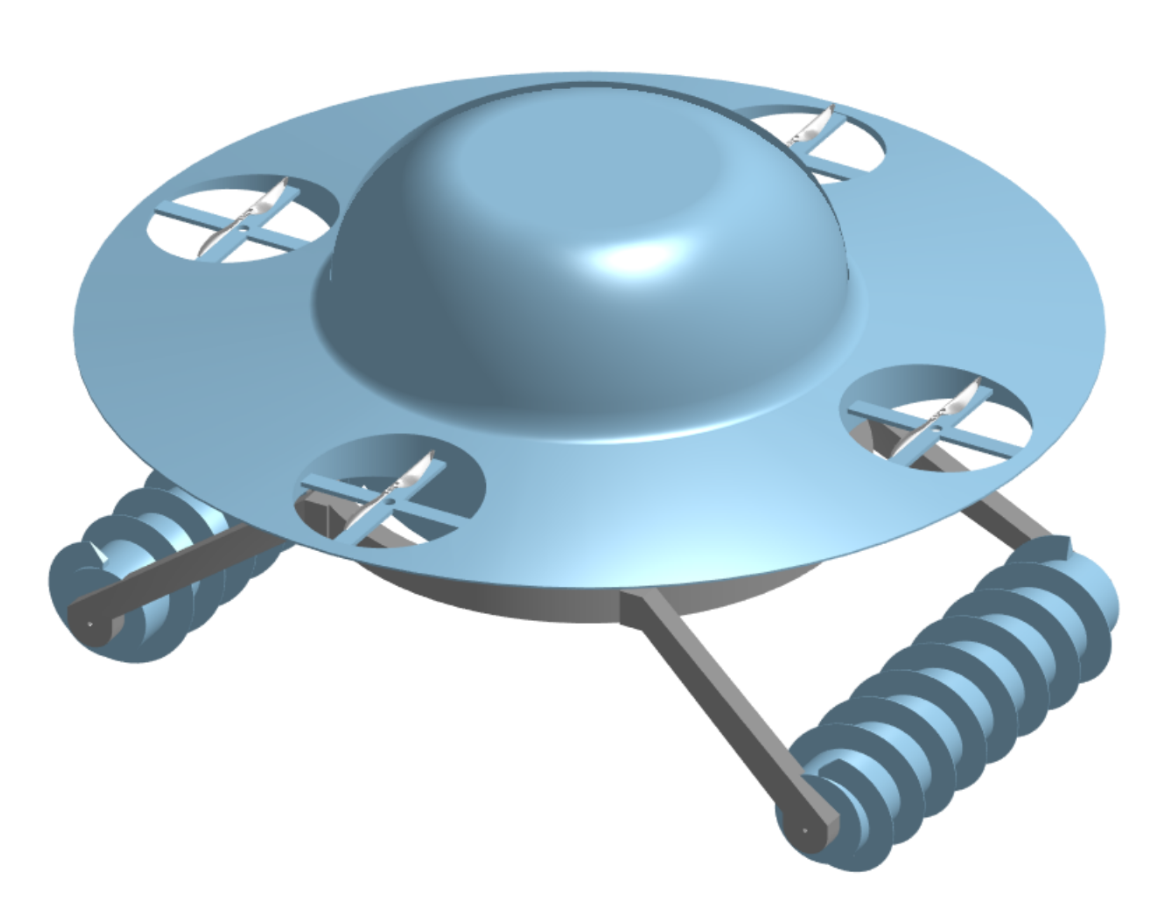
\includegraphics[width=\linewidth]{images/omnibot/omnibot_render_isometric.png}
  \caption{Omnibot Concept} 
  \label{fig:omnibot_render_iso}
  \end{subfigure}
  \begin{subfigure}{0.5\textwidth}
  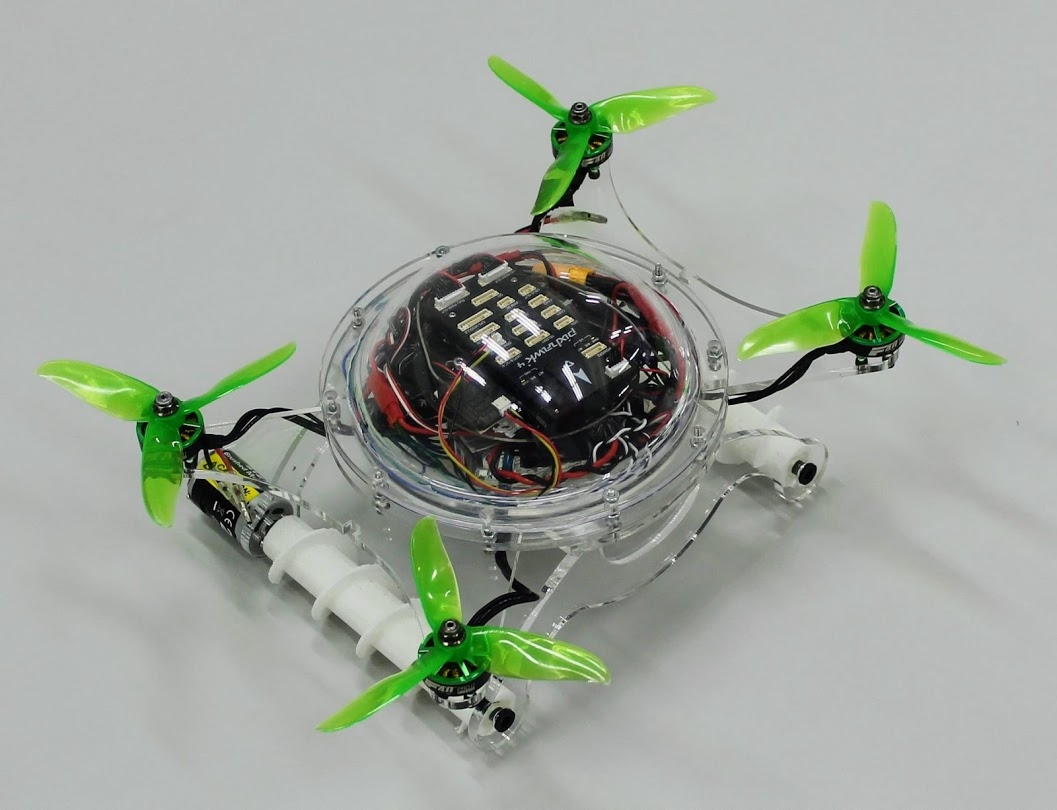
\includegraphics[width=\linewidth]{images/omnibot/omnibot_isometric.jpg}
  \caption{Omnibot Prototype} 
  \label{fig:omnibot_iso}
  \end{subfigure}
  
  \caption{Omnibot Design and Prototype}
  \label{fig:omnibot_prototype_design}

\end{figure}

The Omnibot is proposed as a multi-domain robotic platform for environmental monitoring capable of operating on land, in the air, and in the water. While there are robots capable of land-water, air-ground, and air-water locomotion separately, there is not a platform that performs in all three domains completely. The exception is the multi-field universal wheel for the air-land vehicle (MUWA)\cite{Kawasaki2013}. %Figure \ref{fig:muwa}.

The MUWA is a quad-copter that uses a variable pitch propeller scheme to direct the thrust from its four propellers to achieve VTOL and hover flight. On land, it is able to prop itself up on its outer structure, which consists of styrofoam rings, and function as a wheel, keeping itself upright via propeller thrust. It is also able to float on top of the water but is not capable of underwater navigation due to its permanently positively buyoant nature and construction. 

%\begin{figure}[!ht]
  %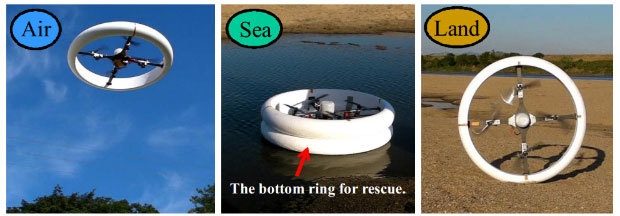
\includegraphics[width=\linewidth]{images/muwa.jpg}
  %\caption{The MUWA model (courtesy of \cite{Kawasaki2013})}
  %\label{fig:muwa}
%\end{figure}

To the author's knowledge, the Omnibot would be the first to navigate all three environments. The benefits would be numerous ranging from leveraging flight for faster travel or to overcome insurpassable obstacles, to landing for more precise measurements, to diving underwater for water quality monitoring, this versality is key to increasing capabilities in real world environments. 

\subsubsection{Prototype Design}

The proposed design will use a waterproof shell to house electronic components, a buoyancy control unit to dive and ascend in water, a dual screwdrive system for navigating land and water, a speed-control quad-rotor design for flight. A removable payload “disk” around its periphery would be used to extend the sensing capabilities of the robot while increasing the craft's aerodynamic properties. Payload disks could be configured with different sensors in order to allow easy deployment of many Omnibots with different capabilities. For example, one could have a payload for water quality measurements, while another could have a communications package and cameras. 

The Omnibot would utilize a NVIDIA Jetson board to simultaneously gather sensor data from a number of cameras pointing up, down, and around its body. This array of cameras would allow omnidirectional proprioception and leading to interesting opportunities for a number of activities such as: crop monitoring on land and air, lake health evaluation from the air, surface, and in the water, search and rescue missions, etc. 

To achieve these ambitious goals, an initial prototype will be built to study and optimize the robot around specific challenges inherent to operation in land, water, and air. Key design contraints are expected to be focused around achieving a weight, volume, and mass balance such that neutral buoyancy can be achieved, all while maintaining a sufficiently low weight to achieve flight within a feasible combination of commercial off the shelf battery, motors, and propellers. 

\begin{figure}[ht]

  \begin{subfigure}{0.5\textwidth}
  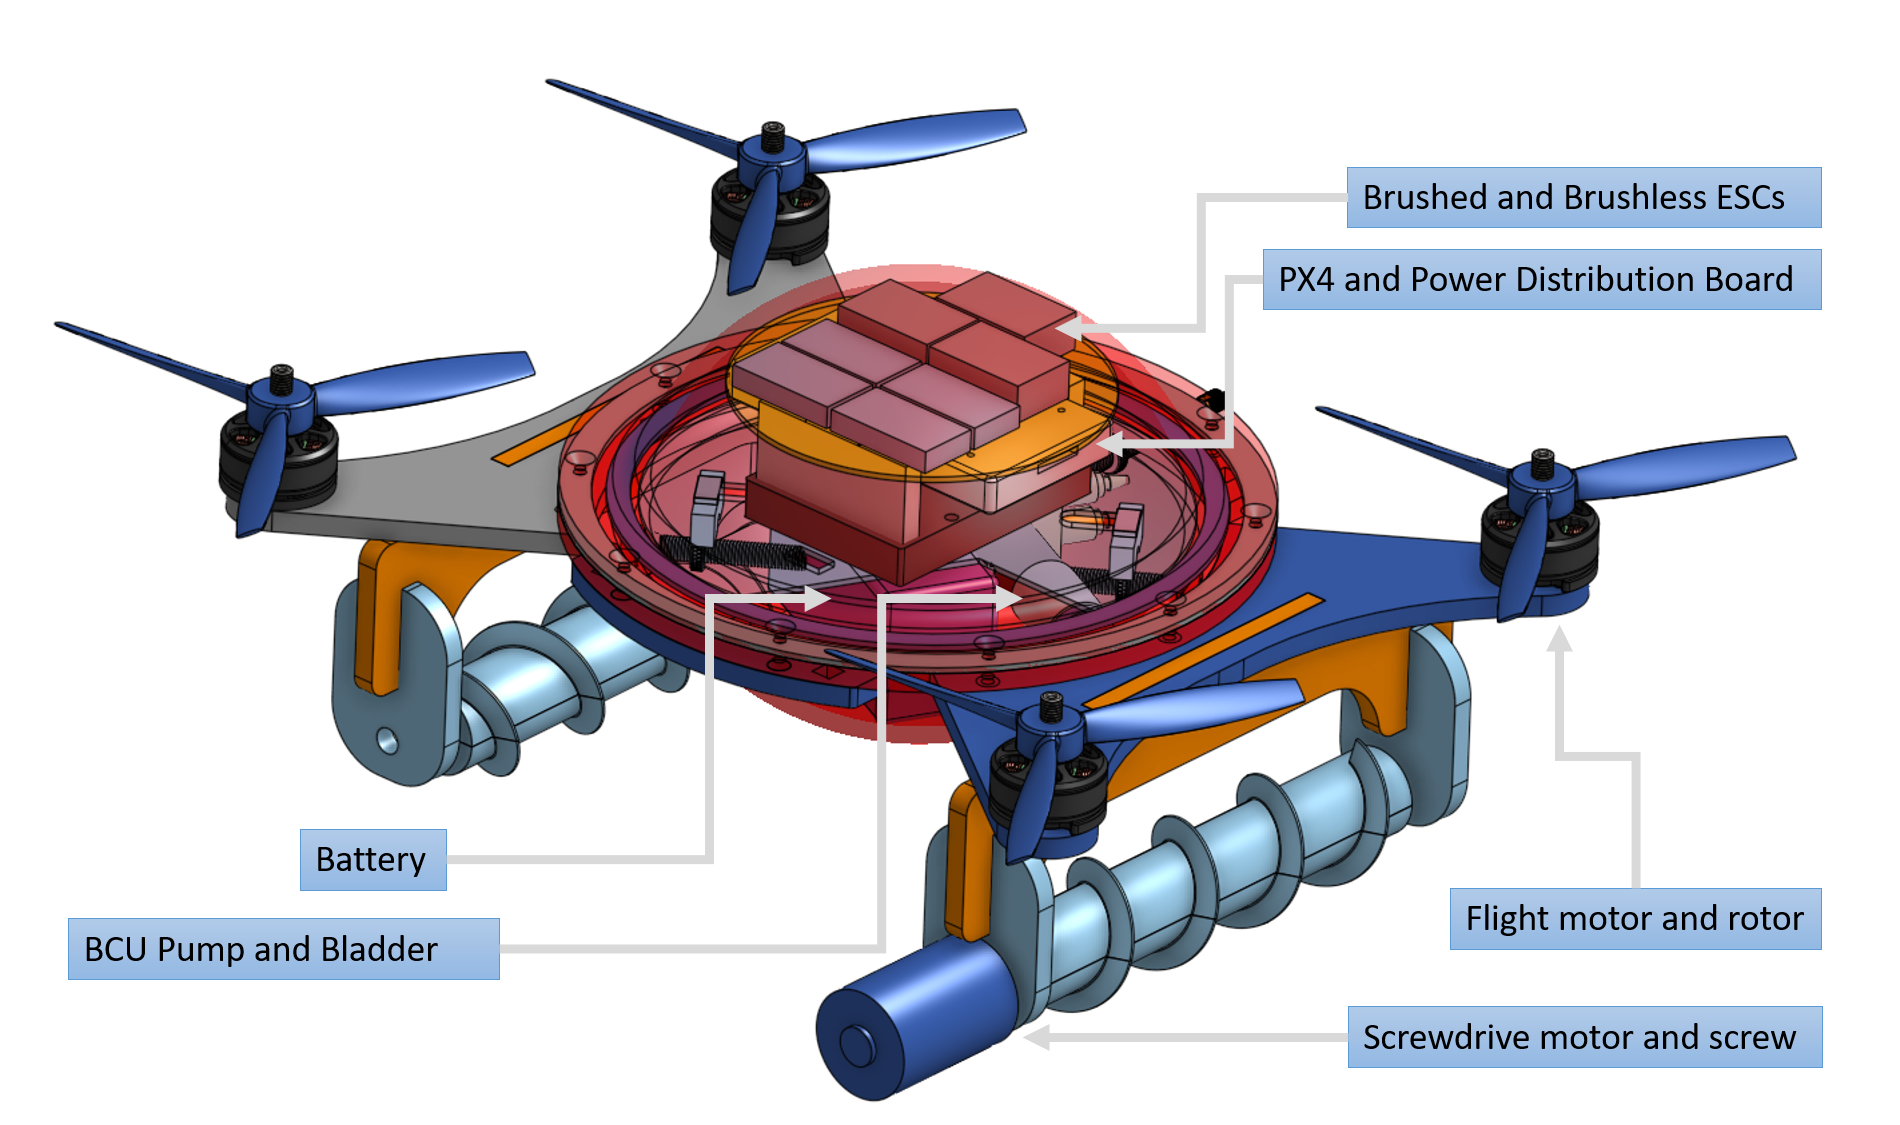
\includegraphics[width=\linewidth]{images/omnibot/omnibot_icuas_annotation.png}
  \caption{Omnibot Annotated Render} 
  \label{fig:omnibot_annotated_render}
  \end{subfigure}
  \begin{subfigure}{0.5\textwidth}
	\includegraphics[width=\columnwidth]{images/omnibot_electrical_schematic_tall.pdf}
  \caption{Omnibot Electronic System Schematic.}
	\label{fig:electronic_schematic} 
  \end{subfigure}

  \caption{Omnibot Design and Prototype}
  \label{fig:omnibot_electronics}

\end{figure}

Once the proof-of-concept prototype is built, the objective is to demonstrate navigation in all three domains as well as the transition between domains. Land-water, land-air, and water-air, as well as their reverse transitions are to be studied as these are expected to present their unique challenges, while being key to robust function. Once the prototype is successful, the next stage is to incorporate the environmental monitoring capabilities. This is expected to be accomplished via the integration of the sensor/payload disk on the periphery of the robot, as well as the integration of a high-level compute board, such as an NVIDIA Jetson board, for onboard processing. %The end result of these efforts would culminate a robot capable of carrying out environmental monitoring tasks in all three environments.  

%By leveraging a new propulsion method for land and water locomotion in conjunction with quad-rotor designs for flight, coupled with a waterproof hull and buoyancy control unit to alter its density, the Omnibot is able to travel on and through water, over land, and in the air. As far as we know, the Omnibot constitutes the first robot that could cover all four typical kinds of environments.

Covering all four mentioned domains presents a special challenge that is more than combining parts. As stated, there exist robotic solutions for each or a couple of domains, however, each has requirements or solutions that can be at odds with the requirements of a different domain. These challenges can be broken into the locomotive, structural, as well as electronic aspects, where locomotive covers the means by which the Omnibot is to move itself through a given media, structural covers the physical properties the platform has to deal with the four types of regions, and electronic is that which pertains to the power distribution, signal, and control of the robot. 
  
\subsubsection{Locomotion}

Central to the functionality and usability of a mobile robotic platform are the methods by which it moves itself through the environment it is in. Often, the aforementioned methods amount to be a fundamental choice as they place constraints on battery life, feasible paths to be followed, and the type of terrain to be traversed, variables which are of critical importance to all mobile platforms with a limited supply of power. 

A dual-parallel screw screwdrive powertrain was chosen for its ability to traverse both land and water environments as shown in Figure~\ref{fig:omnibot_iso}. It employs two independently actuated and contra-rotating continuous propellers. The screws consists of a cylinder with blades forming a helix around its surface. When rotated in a coordinated fashion, these allow a variety of movements. 

For flight, a quad-copter design was chosen based on its ability to provide the necessary amount of thrust, stability, and, most importantly, because vertical-take-off-and-lift (VTOL) allows effective air-ground and air-water transitions. Additionally, VTOL allows the robot to land carefully atop the screwdrive subsystem. When transitioning from water to air, the Omnibot was designed such that the propellers sit above water line. Fixed-wing alternatives would have placed additional and incompatible restrictions on weight, size, and other variables all while increasing the size. 

This design uses the T-Motor F40 Pro II KV2400 motors which weigh 29.5 grams a piece, yet are able to provide a theoretical 1400 grams of thrust when at full throttle and paired with a 4 cell Lithium Polymer battery. Additionally, underwater operation is achievable via a buoyancy control unit, as on the Aquapod. 

\subsubsection{Structural Design}

The majority of the Omnibot's electronic parts are enclosed within an transparent acrylic sphere, which is formed of two transparent hemispheres that clamp onto an O-ring that sits on a custom gland in one of the hemisphere's flanges.  The spherical design was chosen aero and hydrodynamic purposes and the transparency of the enclosure allows for cameras to be added inside without any further modifications.

The enclosure sphere is connected to the flight motors via a set of independent wings that are bolted to the sphere using the same bolting pattern that seals the two hemispheres. These motors are located at the extremities of the wings and are designed such that the DALPROP 4045 tri-blade propellers are sufficiently far away from the robot to avoid collision during flight, but also to allow simple access to the shell. 

The robot itself is suspended 1.1 inches by two screwdrive "legs" which are press fit and acrylic welded orthogonoal to the wings. The clearance is helpful for land navigation purposes. The motors that power the screws bolt on to the legs for ease of access and maintenance. 

A removable payload “disc” around the globe will be used in the future to extend the capabilities of the robot. Mounting different sensor suites to the exterior of the robot, will allow customizability of groups of Omnibots.

The Omnibot weighs approximately 1,418 grams dry and with an empty bladder and its volume is designed such that the robot is 25 grams over the neutral buoyancy point, therefore, within the bladder's water capacity. 

\subsubsection{Electronics and Software }

The prototype is built by integrating off-the-shelf and custom-designed components as seen in Fig.~\ref{fig:electronic_schematic}. At the heart of it all is the 4-cell lithium battery which powers the entire system. The Pixhawk 4 flight controller board \cite{pixhawkadmin_introducing_2018} connects to the GPS/Compass and external remote controller. During flight, it directs signals to the brushless flight motors through the F35A electronic speed controllers. The Pixhawk is also used to send WPM signals to the brushed motors that power the BCU pump as well as the two external brushed motors of the screwdrive system. 

The PX4 flight stack \cite{noauthor_open_nodate} and the Pixhawk 4 were chosen for their versatility and configurability. The PX4 firmware stack is modified to allow powering of the additional actuators but also to add and allow switching between different operational modes: land, water, or air.  

\subsubsection{Laboratory Experiments}
\label{omnibot_experiments_lab}

\begin{figure}[h!]
   \begin{subfigure}[t]{0.30\textwidth}
     \includegraphics[trim=0 40 0 40,clip,width=\textwidth]{images/omnibot/omnibot_lab.png}
     \caption{Land locomotion.}
     \label{fig:omnibot_indoor_land}
   \end{subfigure}
   \begin{subfigure}[t]{0.38\textwidth}
     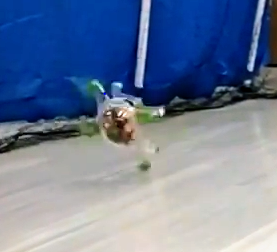
\includegraphics[trim=0 49 0 49,clip,width=\textwidth]{images/omnibot/omnibot_flip.png}
     \caption{Incipient flight.}
     \label{fig:omnibot_flip}
   \end{subfigure}
   \begin{subfigure}[t]{0.30\textwidth}
     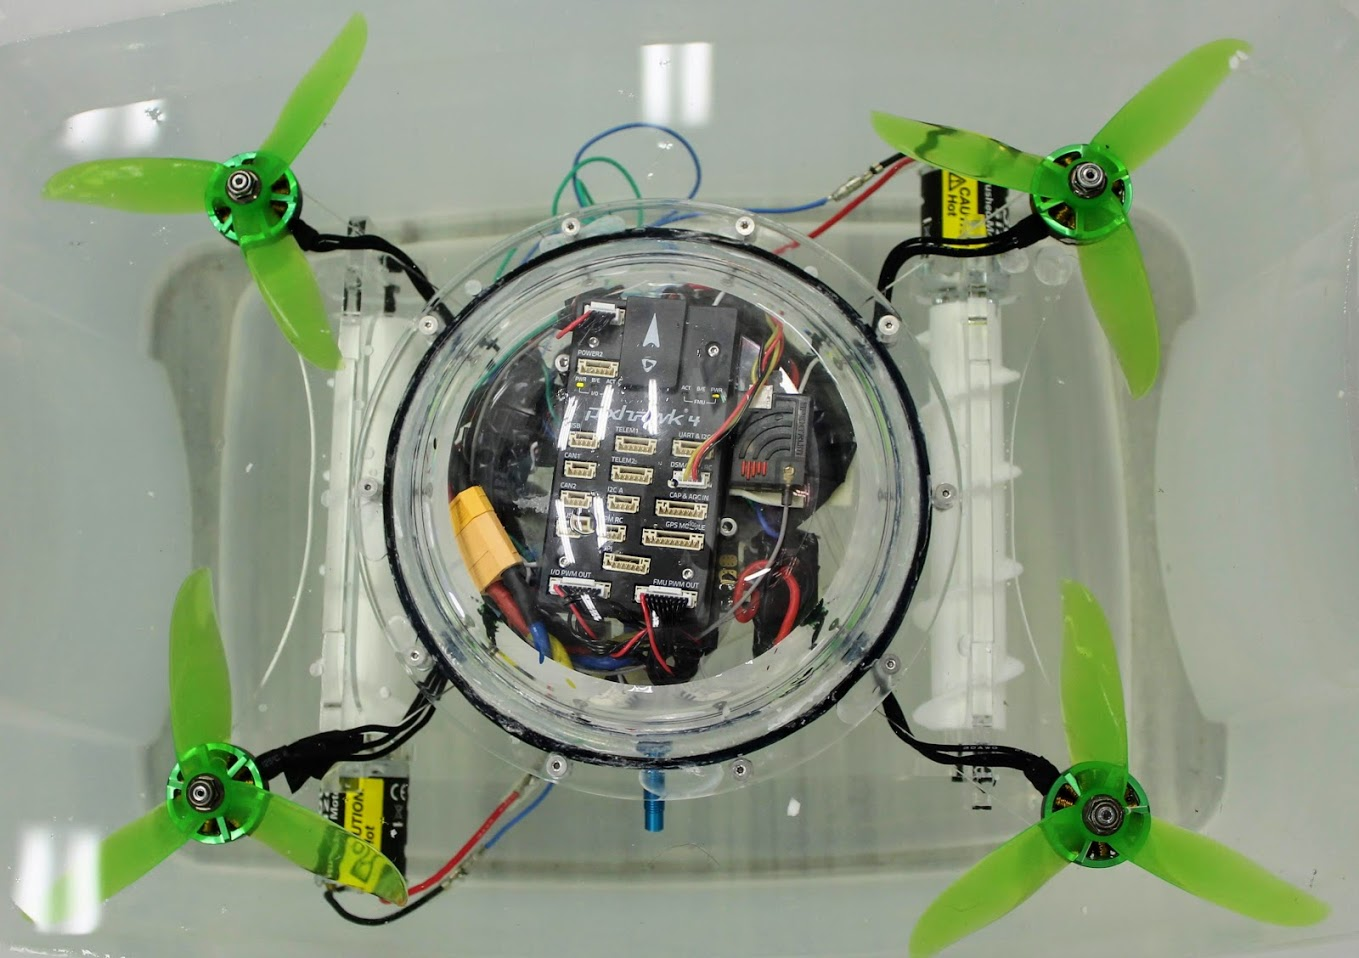
\includegraphics[width=\textwidth]{images/omnibot/omnibot_top.jpg}
     \caption{In water.}
     \label{fig:omnibot_lab_water}
   \end{subfigure}
   \caption{Indoor Omnibot prototype locomotion testing.}
   \label{fig:omnibot_lab}
\end{figure}


%The proof-of-concept model was first tested in each individual environment as shown in Figure ~\ref{fig:omnibot_lab}. 

The first tests involved testing the water-worthiness of the robot. The robot was subjected to bidirectional pressure gradients in order to stress test the main seal as well as the ports' seals. Internal pressure testing was done utilizing a compressed air line and visually verifying no air escaped while submerged in a container. The external pressure test was performed in a similar manner but with pressure provided by hydrostatic water pressure and visually inspecting for water within the clear shell, as can be seen in Fig.~\ref{fig:omnibot_lab_water}. 

Land locomotion was verified in a lab environment on relatively flat but roughly textured floors, as in Fig.~\ref{fig:omnibot_indoor_land}. The objective was to engage the screwdrive system and verify that the movement speed was controllable and adequate. As expected, in an impenetrable terrain of relatively high friction, the screws act like rollers with no tractive effort. 

Air function was verified within a controlled environment surrounded by a protective net. The goal here was to use the remote control to lift the robot off the ground. This test was successful in the Omnibot was able to create enough lift from its propulsion system to take-off from the ground. That being said, there is more work to be done in this area as control and weight balance was an issue. 


\subsubsection{Outdoor Experiments}
\label{omnibot_experiments_outdoor}

\begin{figure*}[h!]
   \begin{subfigure}[t]{0.30\textwidth}
     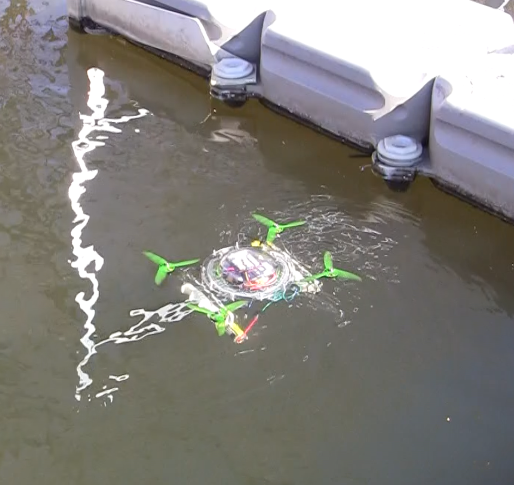
\includegraphics[trim=0 50 0 70,clip,width=\textwidth]{images/omnibot/omnibot_river_dock_small.png}
     \caption{Water operation.}
     \label{fig:omnibot_river}
   \end{subfigure}
   \begin{subfigure}[t]{0.38\textwidth}
     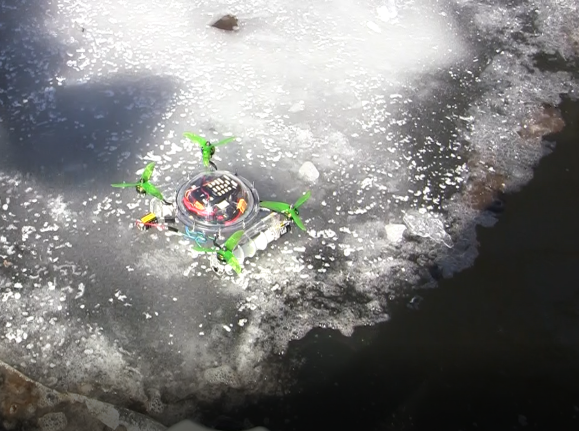
\includegraphics[trim=0 50 0 50,clip,width=\textwidth]{images/omnibot/omnibot_ice_2_small.png}
     \caption{Resting on floating ice.}
     \label{fig:omnibot_ice}
   \end{subfigure}
   \begin{subfigure}[t]{0.30\textwidth}
     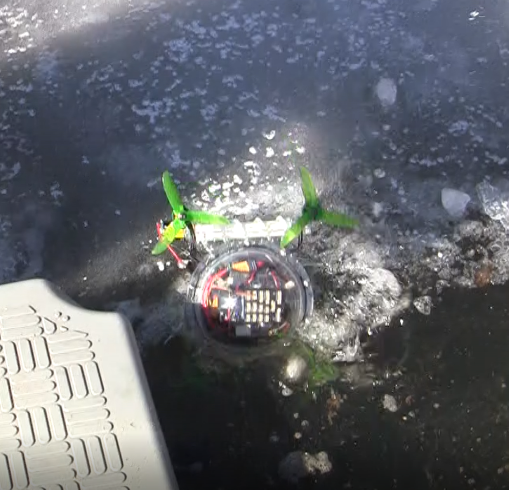
\includegraphics[trim=0 0 0 120,clip,width=\textwidth]{images/omnibot/omnibot_ice_water_transition_small.png}
     \caption{Ice to water transition.}
     \label{fig:omnibot_ice_water}
   \end{subfigure}
   \caption{Outdoor Omnibot prototype testing on the Mississippi River.}
   \label{fig:omnibot_outdoor_test}
\end{figure*}

After indoor testing of the Omnibot in each individual environment, testing in a real-world setting at the docks of the University of Minnesota Boathouse on the Mississippi River was planned. At the time of the experiments river ice was common around the dock and there was a section of floating ice trapped next to the docks that served as a convenient platform for launching the Omnibot (Figure~\ref{fig:omnibot_ice}).  

The outdoor experiments consisted primarily of water navigation, locomotion on ice, and the transition from the floating ice shelf into the water to verify functionality. The first experiment was of the screwdrive for water locomotion (Figure~\ref{fig:omnibot_river}). Next the robot was manually placed on the floating ice and maneuvered in a circle. Lastly, a land to water transition was carried out by driving the robot off the ice and into the cold Mississippi water (Figure ~\ref{fig:omnibot_ice_water}).

The experiments were successful in that they functioned as expected, with the screwdrive system successfully moving the robot in the water, on the ice, and during the launch. To note was the forward traction of the screwdrive on the impenetrable ice, this is though to be due to the low friction between the ice and the screws allowing the robot to ``skate'' on ice.  

%The outdoor experiments were carried out at approximately 27 degrees Farenheit, although the water temperature was not measured, it was as cold, if not colder. This was significant due to the elastomeric nature of the seals, which can shrink and become brittle under low temperatures. 

\subsubsection{Proposed Work}
\label{omnibot_proposed}

We propose creating a novel platform capable of navigating water, land, and air in order to expand the available types of environments that can be monitored and giving unprecedented ability to use the best locomotion type to overcome obstacles and unforeseen circumstances. The platform would be developed to demonstrate:

\begin{itemize}
  \item Operation and seamless transition between all domains.
  \item Integration of sensor payloads for environment monitoring.
  \item Characterization of energy expenditure in each enviroment.
\end{itemize}



%Omnibot background ------------------------------------------------------------------------------------
%On the other hand, there have also emerged a handful of systems that can perform tasks in two or three kinds of regions, making them especially suitable to carry out more complex tasks in varying or changing environments. However, none of them could cover all four common kinds of territories including land, air, water surface and under water.

%Nowadays, various kinds of autonomous systems are being intensively developed and deployed to numerous civil and military application areas. According to their active regions, they can be divided into two groups, specialized robotic platforms including UGVs, UAVs, USVs and UUVs, and multi-purpose ones, which are composed of vehicles that can cover more than one fields. 

%UGVs operate while in contact with the viground. Therefore, they can gather information at a much higher resolution than UAVs. Nonetheless, UGVs are usually much slower in terms speed and efficiency. Furthermore, they are constrained by whatever obstacles may be present in their environment. 

%USVs can float in the water, monitor the water surface, and even look into the water in a limited fashion. They are valuable for oceanography due to its low cost and flexibility compared with other means.

%UUVs are targeted for underwater applications, including seabed surveillance, fish and current monitoring, etc. Nonetheless, they may suffer from communication and power supply issues. Typically these platforms are either tethered or prohibitively expensive due to the sensors required for localization in a GPS-denied environment. Furthermore, these expensive platforms generally require a larger vessel to transport, deploy, and pick up, adding to overall costs. 

%On the other hand, some types of multi-purpose systems have also been proposed, most of which can enter two kinds of regions while few could cover three modes.

%As a matter of fact, robots that can cover two kinds of regions are not rare. One case in point is that of the hybrid air-water microrobot from Chen et al. \cite{Chen2017} which weighs 175 milligrams. This aerial-aquatic microrobot is capable of flapping its wings to propel itself through air and water. The water to air transition is not simple as it has to overcome significant surface force. Moreover, it has to overcome limitations of flapping wing motion to take off from the surface. The microrobot achieves this by igniting a small chemical reaction to propel itself away from the surface of the water.

%Another example is the AQUA \cite{Dudek2007c}, which is a bi-modal amphibious robot that employs flipper-like legs to move from land and into the water. It uses six appendages to propel itself in the water while using a cockroach-like gait when walking on land. The legs are compliant which serves to provide additional terrainability to the robot. 

%On the miniature robotics side of the spectrum, the Aquapod \cite{Dhull2012} is an amphibious robot that moves around by effectuation tumbles on land and using a buoyancy control unit (BCU) in the column of water. 

%Comparatively, few platforms can navigate through more than two regions. The multi-field universal wheel for the air-land vehicle (MUWA) \cite{Kawasaki2013} turns out to be the only example in this category that we could find. As we can see from Figure \ref{fig:muwa}, the MUWA can fly in the air, float on the water and rotate on the land at an arbitrary angle using a specially designed control algorithm. 

%\cite{Siddall2014} AquaMAV
%\cite{Kossett2013} Hybrid 
%\cite{Mintchev} very similar to Alex's hybrid
%\cite{Alzubi2018} Loon Copter 

%Aquatic–aerial unmanned vehicles recently became the focus of many researchers due to their various possible applications. Achieving a fully operational vehicle that is capable of aerial, water- surface, and underwater operations is a significant challenge considering the vehicle's air–water– air transition, propulsion system, and stability underwater.We present in this paper an unconven- tional unmanned hybrid aquatic–aerial quadcopter with active buoyancy control that is capable of aerial flight and water-surface operation, as well as subaquatic diving. We report on the first successful prototype of the vehicle, named the Loon Copter, to provide initial evaluation results of its performance in both mediums. The Loon Copter uses a single set of motors and propellers for both air and underwater maneuvering. It utilizes a ballast system to control vehicle buoyancy and depth underwater, as well as to perform seamless air-to-water and water-to-air transitions. A closed loop control algorithm is utilized for the vehicle's aerial and water-surface stability and maneuver, whereas an open loop control algorithm is used for underwater maneuver. The experi- mental results show a fully operational prototype with six degrees of freedom underwater, stable flight, operation capabilities onwater surface, and agile maneuvering underwater.

%Omnibot background ------------------------------------------------------------------------------------






%intro?:
%When designing a robot around an intended application or class of applications, there are a number of cross-corelated factors that should be taken into account, such as weight, payload, sensors, type of environment, battery size, actuator size, shape of the external structure, type of environment, chemical compatibility, among others that will determine the efficacy of the robot in carrying out the mission. For example, a small inexpensive robot, would not have the ability to carry large sensors or actuators. 

%TODO: move to multi-environments robots. 
%The Multi-field Universal Wheel for Air-land Vehicle (MUWA) \cite{Kawasaki2013}, Fig~\ref{fig:muwa}, almost achieves this feat in that it operates on land, air, and on the \emph{surface} of a body of water. Consisting of a traditional quad-rotor layout, it is surrounded by a dual styrofoam rings on its periphery. The MUWA uses four variable pitch propellers to control thrust and manuever in the air. When on land, it is able to use this differential thrust to stand itself up on its side and roll on the outer rings as a mono-wheel. These outer rings are positively buoyant and enable the robot to float on the surface of the water and the actuators provide ability to move about in a limited fashion. That being said, Kawasaki et al. did not design the robot to be capable of underwater operation.  

%With the Omnibot, the end goal is a platform that can perform environmental monitoring in all three domains, using flight to transport itself quickly between locations and leveraging its unique capabilities to optimally perform the task at hand. This platform would ideally use a multi-rotor design for flight, a buoyancy control unit to alter its density, a waterproof hull to travel through and in water, and a dual screw system to move about on land and in water. 


%Operation in the three domains is more than the combination of parts as constraints for one domain are often at odds with another domain's contraints. Some contraint conflicts are obvious, such as the minimum necessary weight to enable land and water operation versus flight performance. Other constraints, such as neutral buoyancy, are more nuanced, since weight minimization is favorable for flight but ballast weight may be needed to match the platform's displaced volume. 

%In the case of the MUWA robot, its outer flotation rings keep the robot positively buoyant preventing the robot from going underwater. That being said, even if that were not the case, the electronics would have to be not only water resistant, but waterproof. This is generally stated in terms of ingress protection IP Code, where IP61 would be considered resistant to light water, like rain, and IP67 would mean suitable for conditions of immersion at up to 1 meter. 


%Leveraging a new propulsion method for land and water locomotion in conjunction with  quad and octo-rotor designs for flight, the Amphibot will utilize a buoyancy control unit to alter its density and its waterproof hull to travel through and in water, over land, and to fly through the air. 

%A removable payload “disc” around its periphery will be used to extend the capabilities of the robot in various important ways. Its will reduce frictional losses while moving through air and land. Different sensor suites will be mounted on the disk in such a way to allow easy deployment of many Amphibots with different sensor payloads. 

%The Amphibot will utilize a NVIDIA Jetson TX2 board to simultaneously gather sensor data from six cameras: downward-facing, upward-facing, and four around the periphery of the robot. This array of cameras will allow omnidirectional proprioception. Leading to interesting opportunities for a number of activities such as: crop monitoring on land and air, lake health evaluation from the air, surface, and in the water, search and rescue missions, etc. 


%The Aquapod's strengths can be seen in that it leverages its amphibious nature to navigate and perform measurements in both land and water environments.  Compared to the terrestrial Adelopod, it greatly expanded the nature and type of sensing that could now be undertaken. Terrains that were once inaccessible, such as mud, puddles, and snow, were now traversable and environmental monitoring could be undertaken on environments like lakes and streams. 

%$$ \rho_{omnibot} = (mass_{omnibot}+mass_{bladder})/volume_{omnibot} $$ 

%When the mass of the ingested media is enough to alter the OmniBot's density above that of the media it is contained in, it sinks. Reversing this process leads to the robot floating upwards towards the surface. 

%$$ \rho_{omnibot} > \rho_{water} $$
%$$ \frac{\rho_{omnibot}}{\rho_{water} } > 1 $$
%$$ \rho_{water} = 1000 \frac{kg}{m^3} = 1 \frac{g}{cm^3} $$ 



\section{Conclusions}
\label{sec:conclusions}
%Conclusion 
% Provide a concise summary of what will be known when the research has been completed that is not known. It must present the scientific and/or technical merit of the project. 

First we study and propose design principles for small and inexpensive robotic platforms that can perform in multiple environments. Inexpensive robots are desirable to allow multiple robots to be deployed simultaneously. These platforms are meant to help a biologist take measurements so ease-of-use is important, in that regard, simple and easy to use programmability on the field is a key characteristic. 

We designed and built the Aquapod, a small, inexpensive, and amphibious mobile robotic platform that is capable of altering its buoyancy in water to take measurements to up to ten meters of depth. The Aquapod is able to interface mechanically and electrically via backpack modules that can be connected electronically to the onboard computers. One such backpack module is a water sampling module that can take two independent samples at field-programmable depths. 

Secondly we study a relatively novel method of locomotion powered by screws. The screwdrive is conducive to small inexpensive platforms in that it allows the same actuators to be used for both land and water, reducing the weight and size necessary to move adequately in both environments. While screwdrives have been studied and implemented at larger scales, such as replacements for tank tread systems or tractors, they are relatively unexplored in the case of small robots. A system using two screws is adapted to fit the Aquapod platform. 

Screwdrive actuator feedback together with inertial measurements is proposed for actuator characterization and then terrain identification via a time coherent clustering algorithm. Additionally, we propose the use of origami to allow the design and fabrication of screws from planar surfaces using 2D manufacturing methods such as laser cutting. The creation of a variable geometry screw is proposed. Variable screw parameters together with terrain identification would allow live optimization of screw parameters to optimally navigate a given terrain. 

Lastly, we propose a mobile robotic platform capable of navigating underwater, on land, and in the air. To the author's knowledge at the time of this writing, this has not yet been done. This platform would augment existing environmental monitoring capabilities by adding an aerial and oversight perspective. Moreover, this platform would be uniquely suited to pursue its missions in any environment due to its ability to swim on or in water, navigate on land, and use flight to quickly fly between points or over obstacles. Transitions between the different domains, land, water, and air are considered as these place unique design constraints on the system. 






%\chapter{EXTRA}

%\include{parts/appendix}	% appendices

%\bibliography{parts/library,parts/IROS2012,parts/origami,parts/omnibot}
\bibliography{bibs/library,bibs/IROS2012,bibs/origami,bibs/omnibot}
\bibliographystyle{ieeetr}

\chapter*{Biosketch}
%Not more than 1 page, single-spaced and written in narrative format. Should include a summary of previous education, including institutions attended, and research experiences. 

\begin{singlespace}
Originally from Venezuela, I started my undergraduate studies at the University of the Andes in Merida, Venezuela in 2004 in Geological Engineering. Geological Engineering was one of the most sought after Engineering disciplines due to the country's strong petroleum industry, therefore transferring to a different discipline, if necessary, would be simpler than the other way around. Sure enough, after learning about electromagnetism in Physics II, I transferred to Mechanical Engineering. 

Halfway through my undergraduate studies, the opportunity arose to join my family in Minnesota and finish my Bachelor's degree at the University of Minnesota. While pursuing the engaging coursework in Mechanical Engineering, I had the opportunity to work in two separate research labs. In the Hydraulics Laboratory in the Dept. of Bioproducts and Biosystems Engineering, I was in charge of the research and development of a subterranean fluxmeter, a device that measures subterranean fluid flow while being minimally invasive. The fluxmeter was capable of sensing flow values comparable to those recorded by commercial rain gauges. Follwing this, I carried out cell biostabilization research in Prof. Aksan's laboratory using fluorescent microscopy to evaluate human foreskin fibroblast cell viability under a number of adversarial osmotic and temperature conditions, additionally, I created a testing device capable of suspending cells as small as 6 $\mu m $ in diameter in flow to assist in cell viability research. 

I was admitted into the Mechanical Engineering Department's Ph.D. program following my graduation from the undergraduate program in Fall of 2009 and began working in Prof. Papanikolopoulos's Center for Distributed Robotics (CDR) in the summer of 2010. My time at the CDR has been one of great learning across a wide variety of fields, from acquiring depth in Mechanical Engineering topics, to expanding across to topics typically found in Electrical and Computer Engineering, such as embedded system design and programming, development of custom embedded operating systems, integration of a micro Geiger-Muller sensor, as well as design of inexpensive plant growth chambers for genetics research on Arabidopsis thaliana. 

Research in the CDR includes the work on an amphibious robotic platform, the Aquapod. This team effort created a small and inexpensive robot for collecting data from litoral environments where the amphibious nature would permit data collection opportunities not present in other robots. Further research on this platform has led to the screwdrive drivetrain, as well as the Omnibot. The screwdrive locomotion method aims to enhance the locomotive capabilities of the existing Aquapod platform. The Omnibot platform is a sibling platform to the Aquapod yet capable of flight. This platform is the first of its kind and poses a number of technical challenges, however, the benefits in terms of aerial surveillance, loitering, and deployment capabilities cannot be understated.  

%Research Experience and Relevant Coursework
%enter for Distributed Robotics (Dept. of Computer Science) Fall 2010 – Current
%orked on robot design and sensor integration for multiple robots. Some of the projects are expansion of
%he Adelopod drivetrain to include tank treads, mechanical design, sensor and component specification, and
%ystem testing for the Aquapod robotic platform.
%iostabilization Laboratory (Dept. of Mech. Eng.) Spring 2009 – Fall 2009
%tudied human foreskin fibroblast cell viability when subjected to varying osmotic pressures and
%emperatures using fluorescent microscopy and Fourier Transform Infrared Spectrometry (FTIR)
%eveloped a device capable of retaining a suspended cells, as small as 6 um in diameter, while permitting
%luid transport with the purpose of studying cell membrane stability.
%ydraulics Laboratory (Dept. of B.B.E.) Summer 2007 – Fall 2008
%n charge of the research and development of a subterranean fluxmeter. The purpose of the device is to
%easure fluid flow while being minimally invasive. The fluid was also stored in a compartment for
%osterior extraction and chemical analysis. The fluxmeter was designed to be capable of sensing flow
%alues comparable to those recorded by commercial rain gauges.
%ourses and skills
%roficient in Pro/Engineer, ANSYS, C, MATLAB and SimHydraulics.
%ublications
%andeep Dhull, Dario Canelon, Apostolos Kottas, Justin Dancs, Andrew Carlson, and Nikolaos
%apanikolopoulos. "Aquapod: A Small Amphibious Robot with Sampling Capabilities". IEEE
%nternational Conference on Intelligent Robots and Systems (IROS) 2012.
%rett Hemes, Dario Canelon, Justin Dancs and Nikolaos Papanikolopoulos "Robotic Tumbling
%ocomotion: Overview, the Adelopod-T, and Step Climbing Analysis". IEEE International
%onference on Robotics and Automation (ICRA) 2011. 
  
\end{singlespace}

%Graduate Degree Plan
\includepdf[pages=-]{parts/graduate_degree_plan_filled.pdf}


\end{document}		% End of document.


%Written Preliminary Exam

% Content
%The proposal must contain the following sections: a. Cover Page. The cover page must contain the title of the proposal, student’s name, adviser(s)’s name, and the names of the student’s committee members, including which ones will serve as readers. The submission date should also be included.

%b. Project Summary. The Project Summary is a one page, single-spaced summary of the proposed activity. The Project Summary should be a self-contained description of the proposed research. It should include a statement of objectives and methods to be employed. It must address the scientific and/or technical merit of the project, for example, the influence that the results might have on the direction, progress and thinking in relevant scientific or engineering fields. It must also address the appropriateness of the proposed methods, and the logic and feasibility of the research approach.

%The Project Summary should be informative to persons working in the same or related fields and, insofar as possible, understandable to a scientifically or technically literate lay reader.

%c. Project Description. The Project Description is a 30 page (maximum), double-spaced proposal that describes the thesis project. It should include motivation and objectives, background, proposed research, preliminary results, and conclusion. The organization of the document is up to the student, in consultation with the adviser(s). Figures and tables are included in the 30 page limit.


% Background and Motivation
% The background & motivation section should include a critical review of the relevant literature. It should indicate the current state of understanding of the proposed research topic. The review should emphasize how the prior work relates to the proposed study. It should address the significance and limitations of the cited work. If any figures are taken from another publication or a website, they must be referenced explicitly in the caption.


%Objectives
%The objectives section should provide a context for the proposed work as well as specific objectives and expected significance of the Ph.D. dissertation. It should contain a brief overview of the proposed work in relation to the present state of knowledge in the field and to work in progress by others.

%This section should outline the plan of work, including the activities to be undertaken, and a description of experimental and/or computational methods and procedures. It should address what will be done, how it will achieve the proposed objectives, and should contain justification for the approach proposed. The proposed research section should complete the arguments developed earlier and present initial ideas on how to solve the problems posed. Strong proposals avoid repetition and digression. This section (or sections) should relate the proposed activities to the project objectives and provide expected outcomes, including how the proposed research, if successful, will contribute to a greater understanding of the topical area. An assessment of risk should be provided with the proposed research as well as a contingency plan in case a particular research avenue proves inexpedient in some manner. It should present a reasoned path from where the student begins to where they want to be at the end of the research. 

%Proposed Research 
% The proposed research section should complete the arguments developed earlier and present initial ideas on how to solve the problems posed. Avoid repetitions and digressions. It should relate the proposed activities to the project objectives and provide expected outcomes, including how the proposed research, if successful, will contribute to a greater understanding of the topical area. An assessment of risk should be provided with the proposed research as well as a contingency plan in case a particular research avenue proves inexpedient in some manner. It should present a reasoned path from where the student begins to where they want to be at the end of the research.

%Preliminary Results
% The preliminary results section should provide an overview of completed  work including its significance.  

%Conclusion 
% Provide a concise summary of what will be known when the research has been completed that is not known. It must present the scientific and/or technical merit of the project.

%d. References. Reference information is required. Each reference must include the names of all authors (in the same sequence in which they appear in the publication), the article and journal title, book title, volume number, page numbers, and year of publication. Proposers must be especially careful to follow accepted scholarly practices in providing citations for source materials, including websites, relied upon when preparing any section of the proposal. There is no page limitation for the references, but this section must include cited references only. References should be single-spaced, but a blank line between each individual reference is preferred.

% e. Biosketch. A Biosketch of not more than 1 page, single-spaced should be provided. The biosketch should be written in a narrative format and it should include a summary of previous education, including institutions attended, and research experiences.

%f. A copy of your approved Degree Program Form.

%%%%%%%%%%%%%%%%%%%%%%%%%%%%%%%%%%%%%%%%%%%%%%%%%%%%%%%%%%%%%%%%%%%%%%%%%%%%%%%%

%
